\documentclass[12pt]{article}

\title{Studio dell'oscillatore di Van Der Pol \\
	delle sue varianti e delle sue applicazioni}
\author{Simone Balducci, Alessandro Mancini}
\date{}

\usepackage{amsmath}
\usepackage{amsfonts}
\usepackage{amssymb}
\usepackage{amsthm}
\usepackage{braket}
\usepackage{bbold}
\usepackage[margin=2cm]{geometry}
\usepackage{pgfplots}
\usepackage{fancyhdr}
\usepackage{physics}
\usepackage{systeme,mathtools}
\usepackage{graphicx}
\graphicspath{{./}}
\usepackage{float}
\usepackage{relsize}
\usepackage{dsfont}
\usepackage{calligra}
\usepackage{circuitikz}
\usepackage[miktex]{gnuplottex}
\usepackage{epstopdf}
\usepackage[italian]{babel}
\usepackage{float}
\usepackage[utf8]{inputenc}
\usepackage{listings}

\newcommand{\vv}{\vec{v}}
\newcommand{\vw}{\vec{w}}
\newcommand{\vov}{\vec{0_V}}
\newcommand{\vow}{\vec{0_W}}
\newcommand{\vo}{\vec{0}}
\newcommand{\vx}{\vec{x}}
\newcommand{\R}{\Re}
\newcommand{\la}{\lambda}
\newcommand{\bd}{\textbf}
\newcommand{\lang}{\left\langle}
\newcommand{\rang}{\right\rangle}
\newcommand{\lbra}{\left\lbrace}
\newcommand{\rbra}{\right\rbrace}
\newcommand{\ih}{\hat{i}}
\newcommand{\jh}{\hat{j}}
\newcommand{\kh}{\hat{k}}
\newcommand{\nnabla}{\vec{\nabla}}
\newcommand{\vr}{\vec{r}}
\newcommand{\vac}{\vec{a}}
\newcommand{\vf}{\vec{F}}
\newcommand{\vp}{\vec{p}}
\newcommand{\vom}{\vec{\omega}}
\newcommand{\val}{\vec{\alpha}}
\newcommand{\vsr}{\vec{\mathlarger{\mathlarger{\mathlarger{\scriptr}}}}}
\makeatletter
\newcommand*\bigcdot{\mathpalette\bigcdot@{.5}}
\newcommand*\bigcdot@[2]{\mathbin{\vcenter{\hbox{\scalebox{#2}{$\m@th#1\bullet$}}}}}
\makeatother
\def\dbar{{\mathchar'26\mkern-12mu d}}
\DeclareMathAlphabet{\mathcalligra}{T1}{calligra}{m}{n}
\DeclareFontShape{T1}{calligra}{m}{n}{<->s*[2.2]callig15}{}
\newcommand{\scriptr}{\mathcalligra{r}\,}
\newcommand{\boldscriptr}{\pmb{\mathcalligra{r}}\,}

\begin{document}

\maketitle 
\section{Abstract}
L'obiettivo di questo progetto è studiare le proprietà caratteristiche dell'oscillatore di Van Der Pol e verificarle sperimentalmente mediante delle simulazioni numeriche con dei codici scritti in C++. In particolare si vuole osservare il comportamento rigido di questa equazione differenziale e osservare come cambiano le soluzioni variando il timestep. In seguito si vuole calcolare l'ordine di accuratezza del metodo numerico utilizzato per confrontarlo con il valore atteso. \\
Inoltre si vogliono studiare i modelli matematici che applicano i concetti del modello di Van Der Pol e che derivano da esso, quali il modello Zeeman, che descrive la dinamica di una cellula cardiaca o il modello di FitzHugh-Nagumo. Riguardo il modello Zeeman si vuole anche fare una simulazione in cui due cellule si sincronizzano e autosostengono il loro moto stimolandosi a vicenda. \\
Si è anche considerato il problema dell'oscillatore di Van Der Pol forzato, che presenta un comportamento caotico per smorzamenti caratteristici, e si è cercato di riprodurre questo fenomeno mediante una simulazione in C++ e di calcolare l'esponente di Ljapounov, per poi cercare di riprodurre il suono prodotto e confrontarlo con quello atteso, cercando di riprodurre il rumore udito da Van Der Pol e dai suoi colleghi, che portò allo studio del caos deterministico. \\
Infine si vuole parlare dei circuiti elettronici che presentano un comportamento simile a quello descritto dall'equazione di Van Der Pol e si vuole simulare uno di questi su LtSpice, per confronare i risultati ottenuti con gli andamenti attesi.
\section{L'oscillatore di Van Der Pol}
\subsection{Descrizione}
L'oscillatore di Van Der Pol è un sistema dinamico composto da un oscillatore smorzato, descritto dalla seguente equazione:
\begin{equation}
	\ddot{x} - \mu(1-x^2)\dot{x} + x = 0
\end{equation}
dove $x(t)$ indica l'oscillazione nello spazio delle configurazioni in funzione del tempo e $\mu$ è una costante che indica lo smorzamento. Il termine di mezzo dell'equazione è quello responsabile dello smorzamento, e quindi dell'attrito. 
\begin{figure}[H]
	\centering
	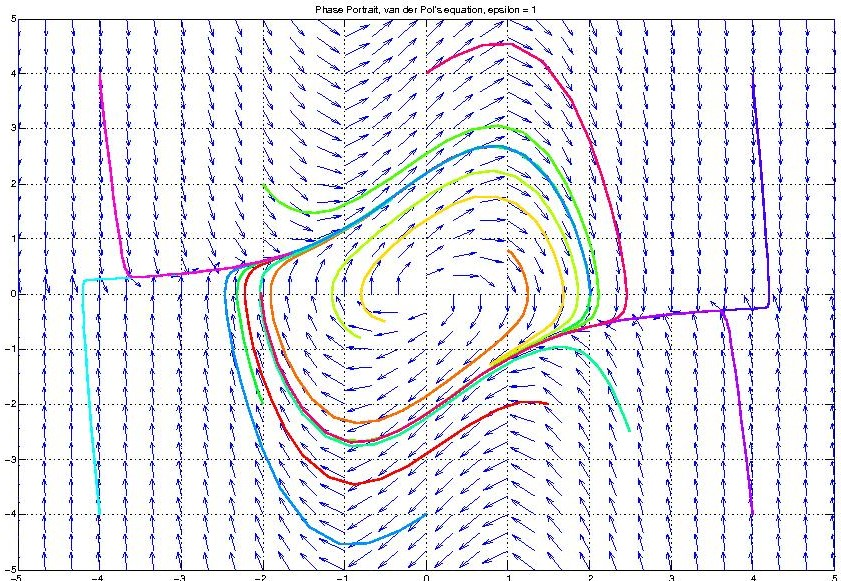
\includegraphics[scale=.4]{Spazio delle fasi oscillatore} 
	\caption{Traiettoria caratteristica dell'oscillatore di Van Der Pol.}
\end{figure}
Si nota subito che nel caso in cui la costante di smorzamento $\mu$ abbia valore nullo, si ottiene un oscillatore armonico classico, e questo verrà verificato nelle sezioni successive mediante simulazioni al computer e esperimenti mediante circuiti elettronici. 
\subsubsection{Studio dell'equazione differenziale}
Consideriamo l'equazione (1) e riscriviamola come:
\begin{equation}
	\ddot{x}+\mu(x^2-1)\dot{x} = \frac{d}{dt}\left(\dot{x}+\mu\left(\frac{1}{3}x^3-x\right)\right) = \frac{d}{dt}\left(\dot{x} + \mu F(x)\right)
\end{equation}
definiamo quindi una nuova variabile
\begin{equation}
	w = \dot{x} + \mu F(x)
\end{equation}
avente derivata 
$$
	\dot{w} = -x
$$
Si ottiene quindi il sistema di equazioni
\begin{equation}
	\begin{cases}
		\dot{x} = w - \mu F(x) \\
		\dot{w} = -x
	\end{cases}
\end{equation}
Studiamo il caso $\dot{x} = 0$, che risulta in
\begin{equation}
	w(x) = \mu F(x) = \mu\left(\frac{1}{3}x^3-x\right)
\end{equation}
e si ottiene quindi una cubica. Studiamo quindi il grafico di questa funzione: 
\begin{figure}[H]
	\centering
	\input{VecField.tex}
	\caption{Grafico che mostra la cubica $F(x)$ e il campo vettoriale $\vec{V}(x,y) = (\dot{x},\dot{y})$.}
\end{figure}
Vediamo che $\dot{w} = 0$ solo per $x=0$, ovvero quando siamo sull'asse delle $y$, e si trova in particolare che sopra l'asse delle $x$ i vettori del campo vettoriale puntano a destra, mentre sotto l'asse delle $x$ puntano a sinistra. Il punto di massimo locale della funzione è $\left(-1,\frac{2}{3}\mu\right)$, mentre il punto di minimo locale è $\left(1,-\frac{2}{3}\mu\right)$. In più vediamo che i punti di intersezione tra le orizzontali che passano per i punti di massimo e minimo con la curva $w$ sono rispettivamente $\left(2,\frac{2}{3}\mu\right)$ $\left(-2,-\frac{2}{3}\mu\right)$. \\
Se consideriamo valori di $\mu$ molto più grandi di 1, vediamo che sarebbe ragionevole riscalare di nuovo le variabili:
\begin{equation}
	y = \frac{w}{\mu} \ \ \Longrightarrow \ \ \begin{cases}
		\dot{x} = \mu(y - F(x)) \\
		\dot{y} = -\frac{1}{\mu}x	
	\end{cases}
\end{equation}
Così si ottiene un grafico uguale a quello di prima ma senza i valori di $\mu$. \\
Fuori dalla curva $\dot{x} = 0$ si ha che $\dot{x}$ è molto grande, mentre $\dot{y}$ è quasi nullo. Questo vuole dire che se mettiamo una particella fuori dalla curva, questa verrà spostata orizzontalmente molto velocemente fino a posizionarsi sulla curva, e subirà anche una piccola accelerazione verticale nella direzione verso la curva. A questo punto la particella si muoverà lentamente sulla curva fino a uno dei vue punti critici, e una volta raggiunti accelererà molto velocemente fino al secondo, in corrispondenza del quale si muoverà molto più lentamente. \\
Si ottiene così un ciclo limite in cui la velocità della particella varia continuamente. In particolare notiamo che più il valore di $\mu$ è grande, più la curva si muoverà lentamente vicino ai punti di minimo/massimo e velocemente lontano da essi. Questo spiega la forma delle traiettorie viste nella figura 4 e sarà inoltre dimostrato visivamente con delle animazioni.
\subsubsection{Studio della stabilità }
Per studiare la stabilità dell'oscillatore di Van Der Pol e la dipendenza della stessa dalla costante di smorzamento $\mu$, si usa il metodo di Lyapunov: \\ \\
\textbf{Primo teorema di Lyapunov: \\}
Per un sistema descritto da un'equazione del tipo 
\begin{equation}
	\dot{\vec{x}} = f(\vec{x},t)
\end{equation}
dove $f(\vo,t) = \vo$ per tutti i $t \geq t_0$, se esiste una funzione scalare $V(\vec{x},t)$ avente derivate parziali continue e che sottisfa le condizioni: 

1) $V(\vec{x},t)$ è definita positiva. 

2) $\dot{V}(\vec{x},t)$ è definita negativa. \\
allora il punto di equilibrio è stabile asintoticamente. \\ \\
Applichiamo ora questo teorema al caso dell'oscillatore di Van Der Pol.  \\
Prima di tutto definiamo una nuova variabile $y = \dot{x}$, in modo da passare da una singola equazione differenziale di secondo ordine a un sistema di due equazioni di primo ordine:
\begin{equation}
	\begin{cases}
		y = \dot{x} \\
		\dot{y} = \mu(1-x^2)y - x
	\end{cases}
\end{equation}
Queste equazioni rappresentano le equazioni del moto dell'oscillatore nello spazio della fasi e possono essere usate per trovare numericamente le traiettorie limite, come si vedrà nella prossima sezione. \\
Consideriamo ora una funzione $V(\vec{x},t)$ del tipo 
\begin{equation}
	V(\vec{x},t) = \frac{1}{2}(x^2 + y^2)
\end{equation}
Questa funzione rispetta la prima caratteristica richiesta dal teorema di Lyapunov, ovvero è definita positiva. Si nota che la costante $1/2$ non era strettamente necessaria, ma è stata aggiunta perchè facendo la derivata totale rispetto al tempo di $V$, questa costante si semplifica e si ritrova il termine dissipativo dell'equazione (1). \\
Ora calcoliamo la derivata della funzione $V$:
$$
	\dot{V}(\vec{x},t) = x\dot{x} + y\dot{y} = x\dot{x} + \mu(1-x^2)\dot{x}^2-x\dot{x} = \mu(1-x^2)\dot{x}^2
$$
\begin{equation}
	\dot{V}(\vec{x},t) = \mu(1-x^2)\dot{x}^2
\end{equation}
Vediamo che in prossimità dell'origine questa funzione è definita negativa se e solo se $\mu$ è negativo. \\
Ne concludiamo quindi che per valori negativi di $\mu$ l'origine è un punto di equilibrio asintotico, e si dice quindi punto attrattivo. \\
Dallo studio della stabilità dell'oscillatore con il metodo di Lyapunov si trova che: 

-Se $\mu>0$, si ha che l'origine è un punto instabile e la particella si allontana da esso, fino ad arrivare su una traiettoria limite che è stabile. Si dice quindi che quella traiettoria è attrattiva. 

-Se $\mu<0$, si ha che l'origine è un punto attrattivo, quindi le traiettorie subiscono una degenerazione attorno ad essa. \\
\begin{figure}[H]
	\centering
	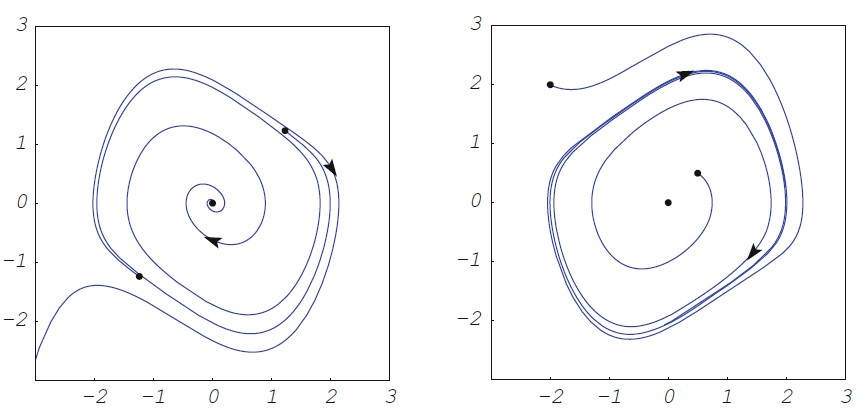
\includegraphics[scale=0.7]{Traiettorie}
	\caption{Traiettorie nello spazio delle fasi, rispettivamente per $\mu$ negativi e positivi.}
\end{figure}
Per valori di $\mu$ positivi, ovvero per cui si hanno delle traiettorie limite che attraggono i punti nello spazio delle fasi, si nota che l'ambiezza di queste curve cresce con lo smorzamento. \\
Come accennato in precedenza, nel caso particolare in cui $\mu = 0$, il sistema si riduce a un oscillatore armonico, quindi la traiettoria sarà una circonferenza.
\begin{figure}[H]
	\centering
	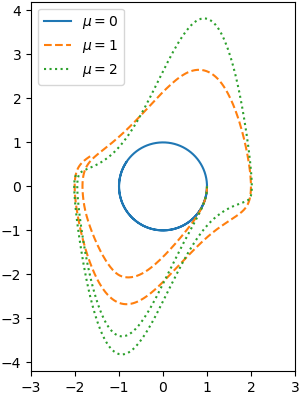
\includegraphics[scale=1]{Vari smorzamenti} 
	\caption{Traiettorie nello spazio delle fasi per vari valori di $\mu$.}
\end{figure} 
\subsection{Applicazioni}
\subsubsection{I neuroni e le cellule cardiace}
Un neurone può creare un potenziale di propagazione, che ha una crescita molto rapida, seguita da una decrescita e una stabilizzazione attorno a uno zero. Mediante la propagazione di questo potenziale il neurone può "comunicare con gli altri neuroni". \\
Le cellule cardiache invece sono cellule muscolari in grado di contrarsi ed estendersi. Tali cellule sono caratterizzate dalla capacità di propagare un segnale (come fanno i neuroni) alle cellule adiacenti, inducendone così la contrazione. Quello che accade di solito è che una prima particella viene eccitata da uno stimolo esterno che ne causa una contrazione, che poi si propaga alle cellule adiacenti, generando una sorta di onda di contrazioni di cellule. Se riportiamo in un grafico la contrazione della cellula cardiaca, $x$, in funzione di un segnale elettrico $b$ che causa la contrazione, cioè lo stimolo esterno, si ottiene un grafico (figura 6) che presenta un comportamento molto simile a quello dell'oscillatore di Van Der Pol:
La contrazione parte lentamente, per poi accentuarsi ad un certo punto, in cui la lunghezza $x$ varia molto velocemente, e questo processo ripetuto crea un moto periodico. \\ \\
Il modello che usiamo per rappresentare questo sistema è
\begin{equation}
	\begin{cases}
		\ \varepsilon \dfrac{dx}{dt} = -(x^3 - Tx + b) \\
		\dfrac{db}{dt} = x - x_0
	\end{cases}
\end{equation}
A questo punto poniamo le derivate nulle e studiamo le nullcline: 
\begin{figure}[H]
	\centering
	% GNUPLOT: LaTeX picture with Postscript
\begingroup
  % Encoding inside the plot.  In the header of your document, this encoding
  % should to defined, e.g., by using
  % \usepackage[cp1252,<other encodings>]{inputenc}
  \inputencoding{cp1252}%
  \makeatletter
  \providecommand\color[2][]{%
    \GenericError{(gnuplot) \space\space\space\@spaces}{%
      Package color not loaded in conjunction with
      terminal option `colourtext'%
    }{See the gnuplot documentation for explanation.%
    }{Either use 'blacktext' in gnuplot or load the package
      color.sty in LaTeX.}%
    \renewcommand\color[2][]{}%
  }%
  \providecommand\includegraphics[2][]{%
    \GenericError{(gnuplot) \space\space\space\@spaces}{%
      Package graphicx or graphics not loaded%
    }{See the gnuplot documentation for explanation.%
    }{The gnuplot epslatex terminal needs graphicx.sty or graphics.sty.}%
    \renewcommand\includegraphics[2][]{}%
  }%
  \providecommand\rotatebox[2]{#2}%
  \@ifundefined{ifGPcolor}{%
    \newif\ifGPcolor
    \GPcolortrue
  }{}%
  \@ifundefined{ifGPblacktext}{%
    \newif\ifGPblacktext
    \GPblacktextfalse
  }{}%
  % define a \g@addto@macro without @ in the name:
  \let\gplgaddtomacro\g@addto@macro
  % define empty templates for all commands taking text:
  \gdef\gplbacktext{}%
  \gdef\gplfronttext{}%
  \makeatother
  \ifGPblacktext
    % no textcolor at all
    \def\colorrgb#1{}%
    \def\colorgray#1{}%
  \else
    % gray or color?
    \ifGPcolor
      \def\colorrgb#1{\color[rgb]{#1}}%
      \def\colorgray#1{\color[gray]{#1}}%
      \expandafter\def\csname LTw\endcsname{\color{white}}%
      \expandafter\def\csname LTb\endcsname{\color{black}}%
      \expandafter\def\csname LTa\endcsname{\color{black}}%
      \expandafter\def\csname LT0\endcsname{\color[rgb]{1,0,0}}%
      \expandafter\def\csname LT1\endcsname{\color[rgb]{0,1,0}}%
      \expandafter\def\csname LT2\endcsname{\color[rgb]{0,0,1}}%
      \expandafter\def\csname LT3\endcsname{\color[rgb]{1,0,1}}%
      \expandafter\def\csname LT4\endcsname{\color[rgb]{0,1,1}}%
      \expandafter\def\csname LT5\endcsname{\color[rgb]{1,1,0}}%
      \expandafter\def\csname LT6\endcsname{\color[rgb]{0,0,0}}%
      \expandafter\def\csname LT7\endcsname{\color[rgb]{1,0.3,0}}%
      \expandafter\def\csname LT8\endcsname{\color[rgb]{0.5,0.5,0.5}}%
    \else
      % gray
      \def\colorrgb#1{\color{black}}%
      \def\colorgray#1{\color[gray]{#1}}%
      \expandafter\def\csname LTw\endcsname{\color{white}}%
      \expandafter\def\csname LTb\endcsname{\color{black}}%
      \expandafter\def\csname LTa\endcsname{\color{black}}%
      \expandafter\def\csname LT0\endcsname{\color{black}}%
      \expandafter\def\csname LT1\endcsname{\color{black}}%
      \expandafter\def\csname LT2\endcsname{\color{black}}%
      \expandafter\def\csname LT3\endcsname{\color{black}}%
      \expandafter\def\csname LT4\endcsname{\color{black}}%
      \expandafter\def\csname LT5\endcsname{\color{black}}%
      \expandafter\def\csname LT6\endcsname{\color{black}}%
      \expandafter\def\csname LT7\endcsname{\color{black}}%
      \expandafter\def\csname LT8\endcsname{\color{black}}%
    \fi
  \fi
    \setlength{\unitlength}{0.0500bp}%
    \ifx\gptboxheight\undefined%
      \newlength{\gptboxheight}%
      \newlength{\gptboxwidth}%
      \newsavebox{\gptboxtext}%
    \fi%
    \setlength{\fboxrule}{0.5pt}%
    \setlength{\fboxsep}{1pt}%
    \definecolor{tbcol}{rgb}{1,1,1}%
\begin{picture}(7936.00,5668.00)%
    \gplgaddtomacro\gplbacktext{%
      \csname LTb\endcsname%%
      \put(726,440){\makebox(0,0)[r]{\strut{}$-1$}}%
      \csname LTb\endcsname%%
      \put(726,1632){\makebox(0,0)[r]{\strut{}$-0.5$}}%
      \csname LTb\endcsname%%
      \put(726,2824){\makebox(0,0)[r]{\strut{}$0$}}%
      \csname LTb\endcsname%%
      \put(726,4016){\makebox(0,0)[r]{\strut{}$0.5$}}%
      \csname LTb\endcsname%%
      \put(726,5209){\makebox(0,0)[r]{\strut{}$1$}}%
      \csname LTb\endcsname%%
      \put(858,220){\makebox(0,0){\strut{}$-2$}}%
      \csname LTb\endcsname%%
      \put(1693,220){\makebox(0,0){\strut{}$-1.5$}}%
      \csname LTb\endcsname%%
      \put(2528,220){\makebox(0,0){\strut{}$-1$}}%
      \csname LTb\endcsname%%
      \put(3363,220){\makebox(0,0){\strut{}$-0.5$}}%
      \csname LTb\endcsname%%
      \put(4199,220){\makebox(0,0){\strut{}$0$}}%
      \csname LTb\endcsname%%
      \put(5034,220){\makebox(0,0){\strut{}$0.5$}}%
      \csname LTb\endcsname%%
      \put(5869,220){\makebox(0,0){\strut{}$1$}}%
      \csname LTb\endcsname%%
      \put(6704,220){\makebox(0,0){\strut{}$1.5$}}%
      \csname LTb\endcsname%%
      \put(7539,220){\makebox(0,0){\strut{}$2$}}%
      \put(3234,1764){\makebox(0,0)[l]{\strut{}B}}%
      \put(5163,3837){\makebox(0,0)[l]{\strut{}A}}%
      \put(6253,1565){\makebox(0,0)[l]{\strut{}(x0,b0)}}%
    }%
    \gplgaddtomacro\gplfronttext{%
      \csname LTb\endcsname%%
      \put(6552,5219){\makebox(0,0)[r]{\strut{}Nullclina x}}%
    }%
    \gplbacktext
    \put(0,0){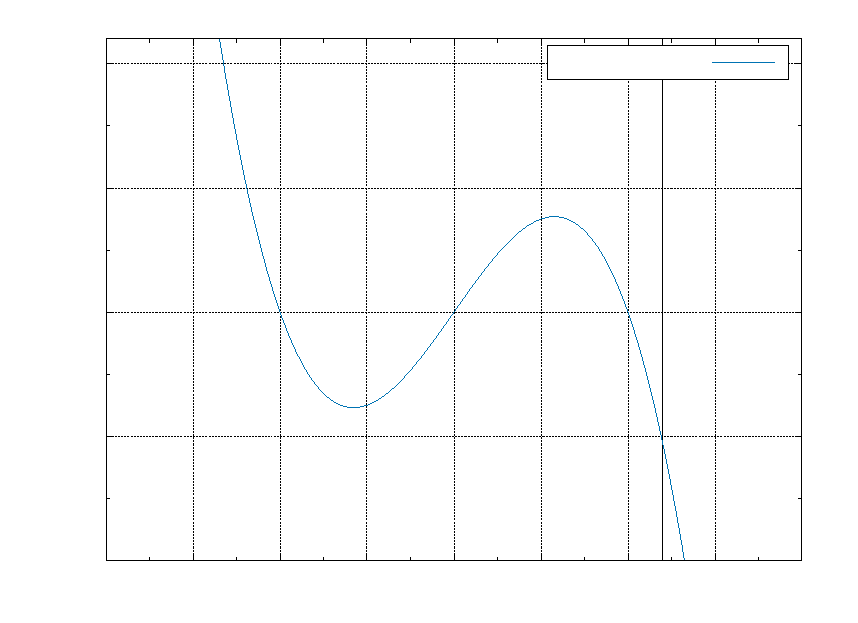
\includegraphics[width={396.80bp},height={283.40bp}]{NeuronNullcline2}}%
    \gplfronttext
  \end{picture}%
\endgroup

	\caption{Nullcline delle equazioni del modello Zeeman.}
\end{figure}
La nullclina della seconda equazione è una retta verticale, mentre la nullclina della prima equazione è una cubica. Le due nullcline si intersecano in un punto di equilibrio $(x_0,b_0)$. \\ 
Essendo tale punto un punto di equilibrio, il sistema tenderà a tornarci quando perturbato da quella condizione. I punti $A$ e $B$ invece sono punti instabili. Vista l'instabilità dei punti $A$ e $B$, se il sistema si avvicina ad essi, esso viene spinto verso il ramo opposto della nullclina molto velocemente, perchè $\varepsilon$ è un parametro piccolo quindi il suo inverso diventa grande. A questo punto il sistema si avvicinerà verso l'altro punto instabile e verrà di nuovo spinto verso l'altro ramo, tornando così al punto di partenza. \\ \\
La dinamica della cellula cardiaca può quindi essere descritta così: La cellula si trova in una condizione iniziale stabile nel punto $(x_0,b_0)$, fino a che uno stimolo esterno non sposta la posizione $x_0$ di equilibrio e porta il sistema verso il punto $A$, da cui poi la particella si contrae violentemente (effetto soglia), per poi tornare spontaneamente alla posizione iniziale. Si capisce quindi che il ramo $AB$ non viene mai percorso. \\ \\
A questo punto si vuole studiare la stabilità del punto di equilibrio. Per fare ciò linearizziamo il problema
$$
	\Delta x = x - x_0 \ \ \ \ \ \ \ \ \ \ \Delta b = b - b_0
$$
e otteniamo il sistema di equazioni
\begin{equation}
	\begin{cases}
		\varepsilon\dfrac{d}{dt}\Delta x = -(3x_0^2 - T)\Delta x - \Delta b \\
		\dfrac{d}{dt} \Delta b = \Delta x
	\end{cases}
\end{equation}
e tale sistema è rappresentabile in forma matriciale
\begin{equation}
	D_t \begin{pmatrix}
		\Delta x \\
		\Delta b
	\end{pmatrix} = \begin{pmatrix}
	\frac{-3x_0^2 + T}{\varepsilon} & -\frac{1}{\varepsilon} \\
	1 & 0
\end{pmatrix} \begin{pmatrix}
	\Delta x \\
	\Delta b
\end{pmatrix}
\end{equation}
Questa matrice ha determinante positivo e uguale a $1/\varepsilon$, e dal momento che in una matrice il determinante è uguale al prodotto degli autovalori, per una matrice $2\times 2$ come questa gli autovalori possono solo essere entrambi positivi o entrambi negativi, e possiamo capire il segno guardando la traccia. Perchè il punto $(x_0,b_0)$ sia stabile gli autovalori devono essere negativi, quindi poniamo la traccia della matrice negativa
$$
	-3x_0^2 + T < 0
$$ 
che da la condizione 
\begin{equation}
	T < 3x_0^2
\end{equation} \\
Si ottiene così che, inserendo nell'equazione una funzione periodica $x^*(t)$, che rappresenta lo stimolo esterno, le equazioni diventano
\begin{equation}
	\begin{cases}
		\ \varepsilon \dfrac{dx}{dt} = -(x^3 - Tx + b) \\
		\dfrac{db}{dt} = x - x^*(t)
	\end{cases}
\end{equation}
e risolvendo questa equazione si ottiene un ciclo molto simile a quello dell'oscillatore di Van Der Pol. 
\begin{figure}[H]
	\centering
	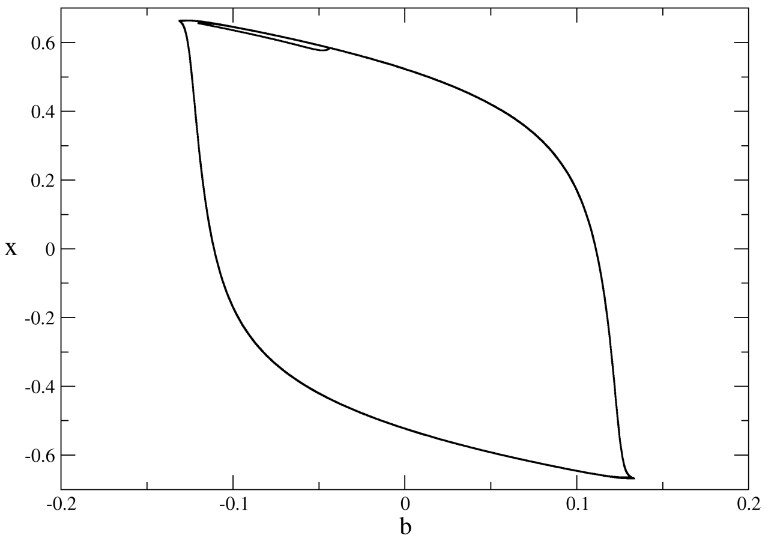
\includegraphics[scale=0.7]{Heartbeat}
	\caption{Traiettoria per una cellula descritta dal modello Zeeman.}
\end{figure}
A questo punto si può pensare di accoppiare due neuroni, e usare la contrazione di uno per stimolare l'altro. Si costruiscono due sistemi descritti dalle seguenti equazioni
\begin{equation}
	\begin{cases}
		\ \varepsilon \dfrac{dx}{dt} = -(x^3 - Tx + b) \\
		\dfrac{db}{dt} = x - y
	\end{cases} \ \ \ \ \ \ \ \ \ \ 
	\begin{cases}
		\ \varepsilon \dfrac{dy}{dt} = -(y^3 - Ty + b') \\
		\dfrac{db'}{dt} = y - x 
	\end{cases}
\end{equation}
e vediamo che così facendo ognuno dei due sente lo stimolo dell'altro, e così riusciamo a sostenere l'onda senza bisogno di uno stimolo esterno. Quindi $b$ e $b'$ non rappresentano più uno stimolo esterno, ad esempio una corrente, bensì rappresentano lo stimolo che un neurone esercita sull'altro. \\
Si è simulata la sincronizzazione di due cellule mediante un codice che risolve prima l'equazione differenziale per una cellula, e usa la soluzione per risolvere l'equazione per la seconda. \\
Nella simulazione si sono usati i seguenti parametri: $T=4$, $\varepsilon=0.01$, $x(0) = 0.65$ e $y(0) = -0.65$ 
\begin{figure}[H]
\ \ \ \ 
\begin{minipage}[b]{0.4\textwidth}
	\centering
	\scalebox{0.7}{% GNUPLOT: LaTeX picture with Postscript
\begingroup
  % Encoding inside the plot.  In the header of your document, this encoding
  % should to defined, e.g., by using
  % \usepackage[cp1252,<other encodings>]{inputenc}
  \inputencoding{cp1252}%
  \makeatletter
  \providecommand\color[2][]{%
    \GenericError{(gnuplot) \space\space\space\@spaces}{%
      Package color not loaded in conjunction with
      terminal option `colourtext'%
    }{See the gnuplot documentation for explanation.%
    }{Either use 'blacktext' in gnuplot or load the package
      color.sty in LaTeX.}%
    \renewcommand\color[2][]{}%
  }%
  \providecommand\includegraphics[2][]{%
    \GenericError{(gnuplot) \space\space\space\@spaces}{%
      Package graphicx or graphics not loaded%
    }{See the gnuplot documentation for explanation.%
    }{The gnuplot epslatex terminal needs graphicx.sty or graphics.sty.}%
    \renewcommand\includegraphics[2][]{}%
  }%
  \providecommand\rotatebox[2]{#2}%
  \@ifundefined{ifGPcolor}{%
    \newif\ifGPcolor
    \GPcolortrue
  }{}%
  \@ifundefined{ifGPblacktext}{%
    \newif\ifGPblacktext
    \GPblacktextfalse
  }{}%
  % define a \g@addto@macro without @ in the name:
  \let\gplgaddtomacro\g@addto@macro
  % define empty templates for all commands taking text:
  \gdef\gplbacktext{}%
  \gdef\gplfronttext{}%
  \makeatother
  \ifGPblacktext
    % no textcolor at all
    \def\colorrgb#1{}%
    \def\colorgray#1{}%
  \else
    % gray or color?
    \ifGPcolor
      \def\colorrgb#1{\color[rgb]{#1}}%
      \def\colorgray#1{\color[gray]{#1}}%
      \expandafter\def\csname LTw\endcsname{\color{white}}%
      \expandafter\def\csname LTb\endcsname{\color{black}}%
      \expandafter\def\csname LTa\endcsname{\color{black}}%
      \expandafter\def\csname LT0\endcsname{\color[rgb]{1,0,0}}%
      \expandafter\def\csname LT1\endcsname{\color[rgb]{0,1,0}}%
      \expandafter\def\csname LT2\endcsname{\color[rgb]{0,0,1}}%
      \expandafter\def\csname LT3\endcsname{\color[rgb]{1,0,1}}%
      \expandafter\def\csname LT4\endcsname{\color[rgb]{0,1,1}}%
      \expandafter\def\csname LT5\endcsname{\color[rgb]{1,1,0}}%
      \expandafter\def\csname LT6\endcsname{\color[rgb]{0,0,0}}%
      \expandafter\def\csname LT7\endcsname{\color[rgb]{1,0.3,0}}%
      \expandafter\def\csname LT8\endcsname{\color[rgb]{0.5,0.5,0.5}}%
    \else
      % gray
      \def\colorrgb#1{\color{black}}%
      \def\colorgray#1{\color[gray]{#1}}%
      \expandafter\def\csname LTw\endcsname{\color{white}}%
      \expandafter\def\csname LTb\endcsname{\color{black}}%
      \expandafter\def\csname LTa\endcsname{\color{black}}%
      \expandafter\def\csname LT0\endcsname{\color{black}}%
      \expandafter\def\csname LT1\endcsname{\color{black}}%
      \expandafter\def\csname LT2\endcsname{\color{black}}%
      \expandafter\def\csname LT3\endcsname{\color{black}}%
      \expandafter\def\csname LT4\endcsname{\color{black}}%
      \expandafter\def\csname LT5\endcsname{\color{black}}%
      \expandafter\def\csname LT6\endcsname{\color{black}}%
      \expandafter\def\csname LT7\endcsname{\color{black}}%
      \expandafter\def\csname LT8\endcsname{\color{black}}%
    \fi
  \fi
    \setlength{\unitlength}{0.0500bp}%
    \ifx\gptboxheight\undefined%
      \newlength{\gptboxheight}%
      \newlength{\gptboxwidth}%
      \newsavebox{\gptboxtext}%
    \fi%
    \setlength{\fboxrule}{0.5pt}%
    \setlength{\fboxsep}{1pt}%
    \definecolor{tbcol}{rgb}{1,1,1}%
\begin{picture}(6802.00,5668.00)%
    \gplgaddtomacro\gplbacktext{%
      \csname LTb\endcsname%%
      \put(682,704){\makebox(0,0)[r]{\strut{}$-4$}}%
      \put(682,1297){\makebox(0,0)[r]{\strut{}$-3$}}%
      \put(682,1890){\makebox(0,0)[r]{\strut{}$-2$}}%
      \put(682,2483){\makebox(0,0)[r]{\strut{}$-1$}}%
      \put(682,3076){\makebox(0,0)[r]{\strut{}$0$}}%
      \put(682,3668){\makebox(0,0)[r]{\strut{}$1$}}%
      \put(682,4261){\makebox(0,0)[r]{\strut{}$2$}}%
      \put(682,4854){\makebox(0,0)[r]{\strut{}$3$}}%
      \put(682,5447){\makebox(0,0)[r]{\strut{}$4$}}%
      \put(814,484){\makebox(0,0){\strut{}$-2.5$}}%
      \put(1373,484){\makebox(0,0){\strut{}$-2$}}%
      \put(1932,484){\makebox(0,0){\strut{}$-1.5$}}%
      \put(2491,484){\makebox(0,0){\strut{}$-1$}}%
      \put(3050,484){\makebox(0,0){\strut{}$-0.5$}}%
      \put(3610,484){\makebox(0,0){\strut{}$0$}}%
      \put(4169,484){\makebox(0,0){\strut{}$0.5$}}%
      \put(4728,484){\makebox(0,0){\strut{}$1$}}%
      \put(5287,484){\makebox(0,0){\strut{}$1.5$}}%
      \put(5846,484){\makebox(0,0){\strut{}$2$}}%
      \put(6405,484){\makebox(0,0){\strut{}$2.5$}}%
    }%
    \gplgaddtomacro\gplfronttext{%
      \csname LTb\endcsname%%
      \put(209,3075){\rotatebox{-270}{\makebox(0,0){\strut{}Stimolo}}}%
      \put(3609,154){\makebox(0,0){\strut{}Contrazione della cellula}}%
      \csname LTb\endcsname%%
      \put(5418,5219){\makebox(0,0)[r]{\strut{}Cellula 1}}%
      \csname LTb\endcsname%%
      \put(5418,4889){\makebox(0,0)[r]{\strut{}Cellula 2}}%
    }%
    \gplbacktext
    \put(0,0){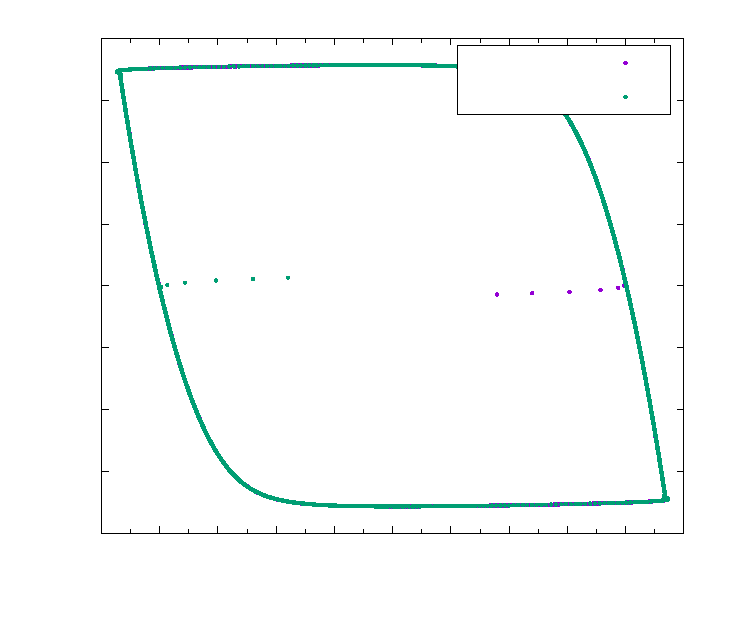
\includegraphics[width={340.10bp},height={283.40bp}]{Sincro}}%
    \gplfronttext
  \end{picture}%
\endgroup
}
	\caption{Cellule sincronizzate (T=4).}
\end{minipage}
\ \ \ \ \ \ \ \ \ \ 
\begin{minipage}[b]{0.4\textwidth}
	\centering
	\scalebox{0.7}{% GNUPLOT: LaTeX picture with Postscript
\begingroup
  % Encoding inside the plot.  In the header of your document, this encoding
  % should to defined, e.g., by using
  % \usepackage[cp1252,<other encodings>]{inputenc}
  \inputencoding{cp1252}%
  \makeatletter
  \providecommand\color[2][]{%
    \GenericError{(gnuplot) \space\space\space\@spaces}{%
      Package color not loaded in conjunction with
      terminal option `colourtext'%
    }{See the gnuplot documentation for explanation.%
    }{Either use 'blacktext' in gnuplot or load the package
      color.sty in LaTeX.}%
    \renewcommand\color[2][]{}%
  }%
  \providecommand\includegraphics[2][]{%
    \GenericError{(gnuplot) \space\space\space\@spaces}{%
      Package graphicx or graphics not loaded%
    }{See the gnuplot documentation for explanation.%
    }{The gnuplot epslatex terminal needs graphicx.sty or graphics.sty.}%
    \renewcommand\includegraphics[2][]{}%
  }%
  \providecommand\rotatebox[2]{#2}%
  \@ifundefined{ifGPcolor}{%
    \newif\ifGPcolor
    \GPcolortrue
  }{}%
  \@ifundefined{ifGPblacktext}{%
    \newif\ifGPblacktext
    \GPblacktextfalse
  }{}%
  % define a \g@addto@macro without @ in the name:
  \let\gplgaddtomacro\g@addto@macro
  % define empty templates for all commands taking text:
  \gdef\gplbacktext{}%
  \gdef\gplfronttext{}%
  \makeatother
  \ifGPblacktext
    % no textcolor at all
    \def\colorrgb#1{}%
    \def\colorgray#1{}%
  \else
    % gray or color?
    \ifGPcolor
      \def\colorrgb#1{\color[rgb]{#1}}%
      \def\colorgray#1{\color[gray]{#1}}%
      \expandafter\def\csname LTw\endcsname{\color{white}}%
      \expandafter\def\csname LTb\endcsname{\color{black}}%
      \expandafter\def\csname LTa\endcsname{\color{black}}%
      \expandafter\def\csname LT0\endcsname{\color[rgb]{1,0,0}}%
      \expandafter\def\csname LT1\endcsname{\color[rgb]{0,1,0}}%
      \expandafter\def\csname LT2\endcsname{\color[rgb]{0,0,1}}%
      \expandafter\def\csname LT3\endcsname{\color[rgb]{1,0,1}}%
      \expandafter\def\csname LT4\endcsname{\color[rgb]{0,1,1}}%
      \expandafter\def\csname LT5\endcsname{\color[rgb]{1,1,0}}%
      \expandafter\def\csname LT6\endcsname{\color[rgb]{0,0,0}}%
      \expandafter\def\csname LT7\endcsname{\color[rgb]{1,0.3,0}}%
      \expandafter\def\csname LT8\endcsname{\color[rgb]{0.5,0.5,0.5}}%
    \else
      % gray
      \def\colorrgb#1{\color{black}}%
      \def\colorgray#1{\color[gray]{#1}}%
      \expandafter\def\csname LTw\endcsname{\color{white}}%
      \expandafter\def\csname LTb\endcsname{\color{black}}%
      \expandafter\def\csname LTa\endcsname{\color{black}}%
      \expandafter\def\csname LT0\endcsname{\color{black}}%
      \expandafter\def\csname LT1\endcsname{\color{black}}%
      \expandafter\def\csname LT2\endcsname{\color{black}}%
      \expandafter\def\csname LT3\endcsname{\color{black}}%
      \expandafter\def\csname LT4\endcsname{\color{black}}%
      \expandafter\def\csname LT5\endcsname{\color{black}}%
      \expandafter\def\csname LT6\endcsname{\color{black}}%
      \expandafter\def\csname LT7\endcsname{\color{black}}%
      \expandafter\def\csname LT8\endcsname{\color{black}}%
    \fi
  \fi
    \setlength{\unitlength}{0.0500bp}%
    \ifx\gptboxheight\undefined%
      \newlength{\gptboxheight}%
      \newlength{\gptboxwidth}%
      \newsavebox{\gptboxtext}%
    \fi%
    \setlength{\fboxrule}{0.5pt}%
    \setlength{\fboxsep}{1pt}%
    \definecolor{tbcol}{rgb}{1,1,1}%
\begin{picture}(6802.00,5668.00)%
    \gplgaddtomacro\gplbacktext{%
      \csname LTb\endcsname%%
      \put(682,704){\makebox(0,0)[r]{\strut{}$-4$}}%
      \put(682,1297){\makebox(0,0)[r]{\strut{}$-3$}}%
      \put(682,1890){\makebox(0,0)[r]{\strut{}$-2$}}%
      \put(682,2483){\makebox(0,0)[r]{\strut{}$-1$}}%
      \put(682,3076){\makebox(0,0)[r]{\strut{}$0$}}%
      \put(682,3668){\makebox(0,0)[r]{\strut{}$1$}}%
      \put(682,4261){\makebox(0,0)[r]{\strut{}$2$}}%
      \put(682,4854){\makebox(0,0)[r]{\strut{}$3$}}%
      \put(682,5447){\makebox(0,0)[r]{\strut{}$4$}}%
      \put(814,484){\makebox(0,0){\strut{}$-2.5$}}%
      \put(1373,484){\makebox(0,0){\strut{}$-2$}}%
      \put(1932,484){\makebox(0,0){\strut{}$-1.5$}}%
      \put(2491,484){\makebox(0,0){\strut{}$-1$}}%
      \put(3050,484){\makebox(0,0){\strut{}$-0.5$}}%
      \put(3610,484){\makebox(0,0){\strut{}$0$}}%
      \put(4169,484){\makebox(0,0){\strut{}$0.5$}}%
      \put(4728,484){\makebox(0,0){\strut{}$1$}}%
      \put(5287,484){\makebox(0,0){\strut{}$1.5$}}%
      \put(5846,484){\makebox(0,0){\strut{}$2$}}%
      \put(6405,484){\makebox(0,0){\strut{}$2.5$}}%
    }%
    \gplgaddtomacro\gplfronttext{%
      \csname LTb\endcsname%%
      \put(209,3075){\rotatebox{-270}{\makebox(0,0){\strut{}Stimolo}}}%
      \put(3609,154){\makebox(0,0){\strut{}Contrazione della cellula}}%
      \csname LTb\endcsname%%
      \put(5418,5219){\makebox(0,0)[r]{\strut{}Cellula 1}}%
      \csname LTb\endcsname%%
      \put(5418,4889){\makebox(0,0)[r]{\strut{}Cellula 2}}%
    }%
    \gplbacktext
    \put(0,0){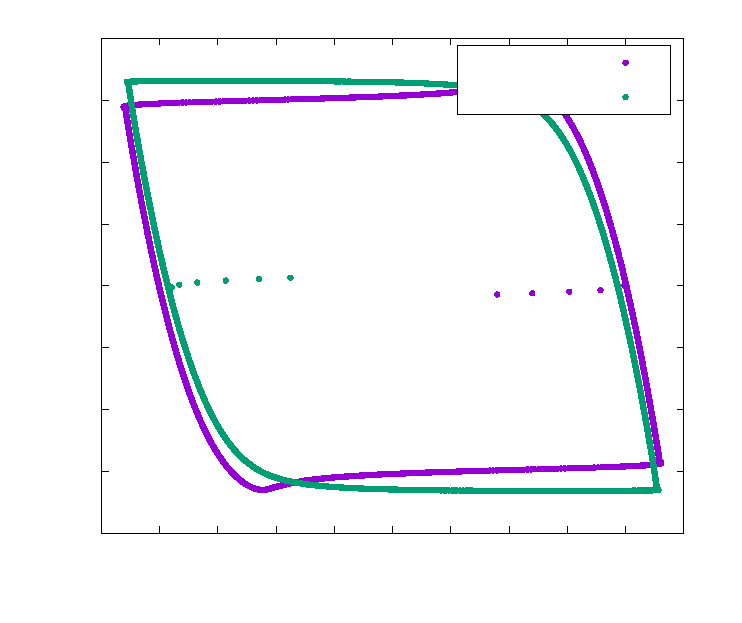
\includegraphics[width={340.10bp},height={283.40bp}]{Sincro3-7}}%
    \gplfronttext
  \end{picture}%
\endgroup
}
	\caption{Cellule con $T_1 = 4$ e $T_2 = 3.7$.}
\end{minipage}
\end{figure}
\begin{figure}[H]
	\ \ \ \ 
	\begin{minipage}[b]{0.4\textwidth}
		\centering
		\scalebox{0.7}{% GNUPLOT: LaTeX picture with Postscript
\begingroup
  % Encoding inside the plot.  In the header of your document, this encoding
  % should to defined, e.g., by using
  % \usepackage[cp1252,<other encodings>]{inputenc}
  \inputencoding{cp1252}%
  \makeatletter
  \providecommand\color[2][]{%
    \GenericError{(gnuplot) \space\space\space\@spaces}{%
      Package color not loaded in conjunction with
      terminal option `colourtext'%
    }{See the gnuplot documentation for explanation.%
    }{Either use 'blacktext' in gnuplot or load the package
      color.sty in LaTeX.}%
    \renewcommand\color[2][]{}%
  }%
  \providecommand\includegraphics[2][]{%
    \GenericError{(gnuplot) \space\space\space\@spaces}{%
      Package graphicx or graphics not loaded%
    }{See the gnuplot documentation for explanation.%
    }{The gnuplot epslatex terminal needs graphicx.sty or graphics.sty.}%
    \renewcommand\includegraphics[2][]{}%
  }%
  \providecommand\rotatebox[2]{#2}%
  \@ifundefined{ifGPcolor}{%
    \newif\ifGPcolor
    \GPcolortrue
  }{}%
  \@ifundefined{ifGPblacktext}{%
    \newif\ifGPblacktext
    \GPblacktextfalse
  }{}%
  % define a \g@addto@macro without @ in the name:
  \let\gplgaddtomacro\g@addto@macro
  % define empty templates for all commands taking text:
  \gdef\gplbacktext{}%
  \gdef\gplfronttext{}%
  \makeatother
  \ifGPblacktext
    % no textcolor at all
    \def\colorrgb#1{}%
    \def\colorgray#1{}%
  \else
    % gray or color?
    \ifGPcolor
      \def\colorrgb#1{\color[rgb]{#1}}%
      \def\colorgray#1{\color[gray]{#1}}%
      \expandafter\def\csname LTw\endcsname{\color{white}}%
      \expandafter\def\csname LTb\endcsname{\color{black}}%
      \expandafter\def\csname LTa\endcsname{\color{black}}%
      \expandafter\def\csname LT0\endcsname{\color[rgb]{1,0,0}}%
      \expandafter\def\csname LT1\endcsname{\color[rgb]{0,1,0}}%
      \expandafter\def\csname LT2\endcsname{\color[rgb]{0,0,1}}%
      \expandafter\def\csname LT3\endcsname{\color[rgb]{1,0,1}}%
      \expandafter\def\csname LT4\endcsname{\color[rgb]{0,1,1}}%
      \expandafter\def\csname LT5\endcsname{\color[rgb]{1,1,0}}%
      \expandafter\def\csname LT6\endcsname{\color[rgb]{0,0,0}}%
      \expandafter\def\csname LT7\endcsname{\color[rgb]{1,0.3,0}}%
      \expandafter\def\csname LT8\endcsname{\color[rgb]{0.5,0.5,0.5}}%
    \else
      % gray
      \def\colorrgb#1{\color{black}}%
      \def\colorgray#1{\color[gray]{#1}}%
      \expandafter\def\csname LTw\endcsname{\color{white}}%
      \expandafter\def\csname LTb\endcsname{\color{black}}%
      \expandafter\def\csname LTa\endcsname{\color{black}}%
      \expandafter\def\csname LT0\endcsname{\color{black}}%
      \expandafter\def\csname LT1\endcsname{\color{black}}%
      \expandafter\def\csname LT2\endcsname{\color{black}}%
      \expandafter\def\csname LT3\endcsname{\color{black}}%
      \expandafter\def\csname LT4\endcsname{\color{black}}%
      \expandafter\def\csname LT5\endcsname{\color{black}}%
      \expandafter\def\csname LT6\endcsname{\color{black}}%
      \expandafter\def\csname LT7\endcsname{\color{black}}%
      \expandafter\def\csname LT8\endcsname{\color{black}}%
    \fi
  \fi
    \setlength{\unitlength}{0.0500bp}%
    \ifx\gptboxheight\undefined%
      \newlength{\gptboxheight}%
      \newlength{\gptboxwidth}%
      \newsavebox{\gptboxtext}%
    \fi%
    \setlength{\fboxrule}{0.5pt}%
    \setlength{\fboxsep}{1pt}%
    \definecolor{tbcol}{rgb}{1,1,1}%
\begin{picture}(6802.00,5668.00)%
    \gplgaddtomacro\gplbacktext{%
      \csname LTb\endcsname%%
      \put(682,704){\makebox(0,0)[r]{\strut{}$-4$}}%
      \put(682,1297){\makebox(0,0)[r]{\strut{}$-3$}}%
      \put(682,1890){\makebox(0,0)[r]{\strut{}$-2$}}%
      \put(682,2483){\makebox(0,0)[r]{\strut{}$-1$}}%
      \put(682,3076){\makebox(0,0)[r]{\strut{}$0$}}%
      \put(682,3668){\makebox(0,0)[r]{\strut{}$1$}}%
      \put(682,4261){\makebox(0,0)[r]{\strut{}$2$}}%
      \put(682,4854){\makebox(0,0)[r]{\strut{}$3$}}%
      \put(682,5447){\makebox(0,0)[r]{\strut{}$4$}}%
      \put(814,484){\makebox(0,0){\strut{}$-2$}}%
      \put(1435,484){\makebox(0,0){\strut{}$-1.5$}}%
      \put(2056,484){\makebox(0,0){\strut{}$-1$}}%
      \put(2678,484){\makebox(0,0){\strut{}$-0.5$}}%
      \put(3299,484){\makebox(0,0){\strut{}$0$}}%
      \put(3920,484){\makebox(0,0){\strut{}$0.5$}}%
      \put(4541,484){\makebox(0,0){\strut{}$1$}}%
      \put(5163,484){\makebox(0,0){\strut{}$1.5$}}%
      \put(5784,484){\makebox(0,0){\strut{}$2$}}%
      \put(6405,484){\makebox(0,0){\strut{}$2.5$}}%
    }%
    \gplgaddtomacro\gplfronttext{%
      \csname LTb\endcsname%%
      \put(209,3075){\rotatebox{-270}{\makebox(0,0){\strut{}Stimolo}}}%
      \put(3609,154){\makebox(0,0){\strut{}Contrazione della cellula}}%
      \csname LTb\endcsname%%
      \put(5418,5219){\makebox(0,0)[r]{\strut{}Cellula 1}}%
      \csname LTb\endcsname%%
      \put(5418,4889){\makebox(0,0)[r]{\strut{}Cellula 2}}%
    }%
    \gplbacktext
    \put(0,0){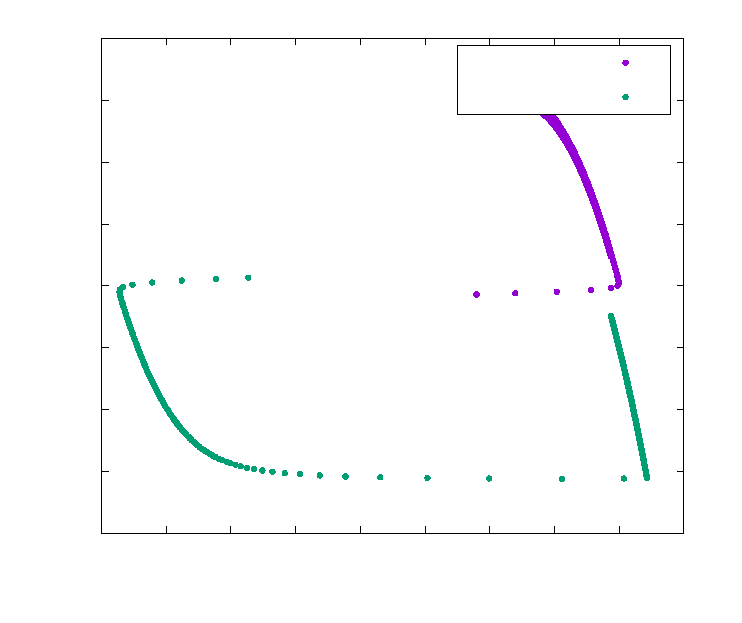
\includegraphics[width={340.10bp},height={283.40bp}]{Sincro3-5}}%
    \gplfronttext
  \end{picture}%
\endgroup
}
		\caption{Cellule con $T_1 = 4$ e $T_2 = 3.5$.}
	\end{minipage}
	\ \ \ \ \ \ \ \ \ \ 
	\begin{minipage}[b]{0.4\textwidth}
		\centering
		\scalebox{0.7}{% GNUPLOT: LaTeX picture with Postscript
\begingroup
  % Encoding inside the plot.  In the header of your document, this encoding
  % should to defined, e.g., by using
  % \usepackage[cp1252,<other encodings>]{inputenc}
  \inputencoding{cp1252}%
  \makeatletter
  \providecommand\color[2][]{%
    \GenericError{(gnuplot) \space\space\space\@spaces}{%
      Package color not loaded in conjunction with
      terminal option `colourtext'%
    }{See the gnuplot documentation for explanation.%
    }{Either use 'blacktext' in gnuplot or load the package
      color.sty in LaTeX.}%
    \renewcommand\color[2][]{}%
  }%
  \providecommand\includegraphics[2][]{%
    \GenericError{(gnuplot) \space\space\space\@spaces}{%
      Package graphicx or graphics not loaded%
    }{See the gnuplot documentation for explanation.%
    }{The gnuplot epslatex terminal needs graphicx.sty or graphics.sty.}%
    \renewcommand\includegraphics[2][]{}%
  }%
  \providecommand\rotatebox[2]{#2}%
  \@ifundefined{ifGPcolor}{%
    \newif\ifGPcolor
    \GPcolortrue
  }{}%
  \@ifundefined{ifGPblacktext}{%
    \newif\ifGPblacktext
    \GPblacktextfalse
  }{}%
  % define a \g@addto@macro without @ in the name:
  \let\gplgaddtomacro\g@addto@macro
  % define empty templates for all commands taking text:
  \gdef\gplbacktext{}%
  \gdef\gplfronttext{}%
  \makeatother
  \ifGPblacktext
    % no textcolor at all
    \def\colorrgb#1{}%
    \def\colorgray#1{}%
  \else
    % gray or color?
    \ifGPcolor
      \def\colorrgb#1{\color[rgb]{#1}}%
      \def\colorgray#1{\color[gray]{#1}}%
      \expandafter\def\csname LTw\endcsname{\color{white}}%
      \expandafter\def\csname LTb\endcsname{\color{black}}%
      \expandafter\def\csname LTa\endcsname{\color{black}}%
      \expandafter\def\csname LT0\endcsname{\color[rgb]{1,0,0}}%
      \expandafter\def\csname LT1\endcsname{\color[rgb]{0,1,0}}%
      \expandafter\def\csname LT2\endcsname{\color[rgb]{0,0,1}}%
      \expandafter\def\csname LT3\endcsname{\color[rgb]{1,0,1}}%
      \expandafter\def\csname LT4\endcsname{\color[rgb]{0,1,1}}%
      \expandafter\def\csname LT5\endcsname{\color[rgb]{1,1,0}}%
      \expandafter\def\csname LT6\endcsname{\color[rgb]{0,0,0}}%
      \expandafter\def\csname LT7\endcsname{\color[rgb]{1,0.3,0}}%
      \expandafter\def\csname LT8\endcsname{\color[rgb]{0.5,0.5,0.5}}%
    \else
      % gray
      \def\colorrgb#1{\color{black}}%
      \def\colorgray#1{\color[gray]{#1}}%
      \expandafter\def\csname LTw\endcsname{\color{white}}%
      \expandafter\def\csname LTb\endcsname{\color{black}}%
      \expandafter\def\csname LTa\endcsname{\color{black}}%
      \expandafter\def\csname LT0\endcsname{\color{black}}%
      \expandafter\def\csname LT1\endcsname{\color{black}}%
      \expandafter\def\csname LT2\endcsname{\color{black}}%
      \expandafter\def\csname LT3\endcsname{\color{black}}%
      \expandafter\def\csname LT4\endcsname{\color{black}}%
      \expandafter\def\csname LT5\endcsname{\color{black}}%
      \expandafter\def\csname LT6\endcsname{\color{black}}%
      \expandafter\def\csname LT7\endcsname{\color{black}}%
      \expandafter\def\csname LT8\endcsname{\color{black}}%
    \fi
  \fi
    \setlength{\unitlength}{0.0500bp}%
    \ifx\gptboxheight\undefined%
      \newlength{\gptboxheight}%
      \newlength{\gptboxwidth}%
      \newsavebox{\gptboxtext}%
    \fi%
    \setlength{\fboxrule}{0.5pt}%
    \setlength{\fboxsep}{1pt}%
    \definecolor{tbcol}{rgb}{1,1,1}%
\begin{picture}(6802.00,5668.00)%
    \gplgaddtomacro\gplbacktext{%
      \csname LTb\endcsname%%
      \put(946,704){\makebox(0,0)[r]{\strut{}$-2.5$}}%
      \put(946,1178){\makebox(0,0)[r]{\strut{}$-2$}}%
      \put(946,1653){\makebox(0,0)[r]{\strut{}$-1.5$}}%
      \put(946,2127){\makebox(0,0)[r]{\strut{}$-1$}}%
      \put(946,2601){\makebox(0,0)[r]{\strut{}$-0.5$}}%
      \put(946,3076){\makebox(0,0)[r]{\strut{}$0$}}%
      \put(946,3550){\makebox(0,0)[r]{\strut{}$0.5$}}%
      \put(946,4024){\makebox(0,0)[r]{\strut{}$1$}}%
      \put(946,4498){\makebox(0,0)[r]{\strut{}$1.5$}}%
      \put(946,4973){\makebox(0,0)[r]{\strut{}$2$}}%
      \put(946,5447){\makebox(0,0)[r]{\strut{}$2.5$}}%
      \put(1078,484){\makebox(0,0){\strut{}$-1$}}%
      \put(1839,484){\makebox(0,0){\strut{}$-0.5$}}%
      \put(2600,484){\makebox(0,0){\strut{}$0$}}%
      \put(3361,484){\makebox(0,0){\strut{}$0.5$}}%
      \put(4122,484){\makebox(0,0){\strut{}$1$}}%
      \put(4883,484){\makebox(0,0){\strut{}$1.5$}}%
      \put(5644,484){\makebox(0,0){\strut{}$2$}}%
      \put(6405,484){\makebox(0,0){\strut{}$2.5$}}%
    }%
    \gplgaddtomacro\gplfronttext{%
      \csname LTb\endcsname%%
      \put(209,3075){\rotatebox{-270}{\makebox(0,0){\strut{}Stimolo}}}%
      \put(3741,154){\makebox(0,0){\strut{}Contrazione della cellula}}%
      \csname LTb\endcsname%%
      \put(5418,5219){\makebox(0,0)[r]{\strut{}Cellula 1}}%
      \csname LTb\endcsname%%
      \put(5418,4889){\makebox(0,0)[r]{\strut{}Cellula 2}}%
    }%
    \gplbacktext
    \put(0,0){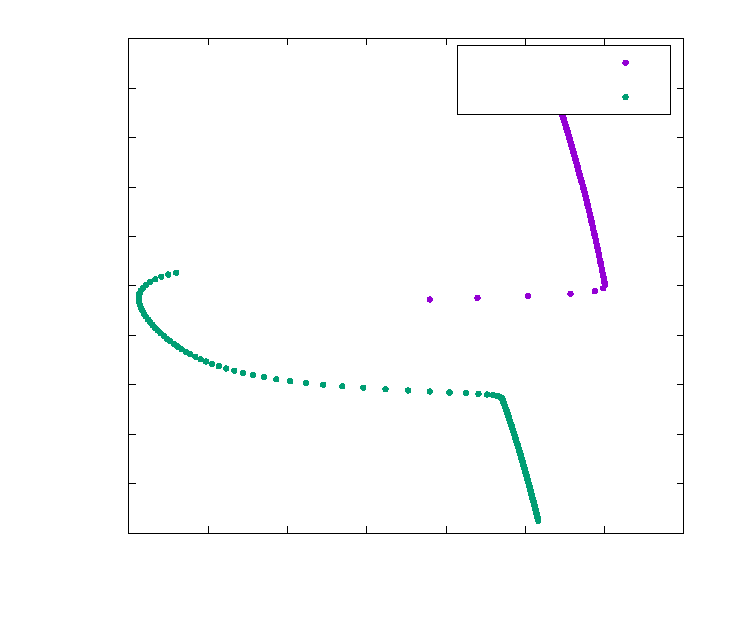
\includegraphics[width={340.10bp},height={283.40bp}]{Sincro2}}%
    \gplfronttext
  \end{picture}%
\endgroup
}
		\caption{Cellule con $T_1 = 4$ e $T_2 = 2$.}
	\end{minipage}
\end{figure}
A questo punto si potrebbe creare una catena di neuroni, dove il primo viene stimolato da uno stimolo esterno, il secondo viene stimolato dal primo e a sua volta stimola il terzo e così via, creando così un'onda.
\subsubsection{Il modello di FitzHugh-Nagumo}
Il modello migliore e più preciso dal punto di vista fisiologico per descrivere un neurone è il modello di Hodgkin-Huxley. Tuttavia questo modello presenta diverse complicazioni, la principale delle quali è la sua estrema non linearità, che esibisce comportamenti caotici che sono difficili da studiare in quattro dimensioni. \\
Per quanto detto, di solito si utilizza una versione semplificata di questo modello che deriva dall'oscillatore di Van Der Pol, cioè il modello di FitzHugh-Nagumo. Questo modello può essere visto come la proiezione bidimensionale del modello di Hodgkin-Huxley. \\ \\
Come detto, il modello di FitzHugh-Nagumo deriva dal modello di Van Der Pol, e infatti le equazioni che lo descrivono hanno una struttura molto simile:
\begin{equation}
	\begin{cases}
		\dot{V} = V - \dfrac{V^3}{3} - W + I \\
		\dot{W} = \dfrac{1}{\tau} \left(V -bW + a\right) 
	\end{cases}
\end{equation}
dove la $V$ rappresenta la variabile veloce, ovvero la variabile che cambia più velocemente, che presenta una dinamica piccata di quasi-soglia, e rappresenta il potenziale di membrana. La $W$ è la variabile lenta, che si chiama variabile di recupero, e rappresenta la caratteristica refrattarietà del neurone dopo essersi eccitato, infatti si chiama variabile di recupero. La separazione tra le due scale temporali è dettata dal parametro $\tau$, perchè $\tau$ è grande, quindi il suo opposto è piccolo, e questo rallenta la variabile $W$. $I$ è uno stimolo esterno, che può rappresentare le correnti date dalle interazioni con gli altri neuroni o dagli stimoli esterni. Infine $a$ è un parametro dinamico che regola il regime dinamico del modello. \\ \\
Studiamo di nuovo le nullcline di questo problema:
$$
	W = x - \frac{x^3}{3} + I \ \ \ \ \ \ \ \ \ \ W = \frac{x+a}{b}
$$
A questo punto, lo stimolo definisce l'intersezione tra l'asse e la cubica, quindi agendo su esso possiamo spostare in alto o in basso la nullclina cubica. \\
L'intersezione tra le due nullcline rappresenta i punti di equilibrio, e in questo caso si ha un solo equilibrio (anche se potrebbero essere di più). 
\begin{figure}[H]
	\centering
	% GNUPLOT: LaTeX picture with Postscript
\begingroup
  % Encoding inside the plot.  In the header of your document, this encoding
  % should to defined, e.g., by using
  % \usepackage[cp1252,<other encodings>]{inputenc}
  \inputencoding{cp1252}%
  \makeatletter
  \providecommand\color[2][]{%
    \GenericError{(gnuplot) \space\space\space\@spaces}{%
      Package color not loaded in conjunction with
      terminal option `colourtext'%
    }{See the gnuplot documentation for explanation.%
    }{Either use 'blacktext' in gnuplot or load the package
      color.sty in LaTeX.}%
    \renewcommand\color[2][]{}%
  }%
  \providecommand\includegraphics[2][]{%
    \GenericError{(gnuplot) \space\space\space\@spaces}{%
      Package graphicx or graphics not loaded%
    }{See the gnuplot documentation for explanation.%
    }{The gnuplot epslatex terminal needs graphicx.sty or graphics.sty.}%
    \renewcommand\includegraphics[2][]{}%
  }%
  \providecommand\rotatebox[2]{#2}%
  \@ifundefined{ifGPcolor}{%
    \newif\ifGPcolor
    \GPcolortrue
  }{}%
  \@ifundefined{ifGPblacktext}{%
    \newif\ifGPblacktext
    \GPblacktextfalse
  }{}%
  % define a \g@addto@macro without @ in the name:
  \let\gplgaddtomacro\g@addto@macro
  % define empty templates for all commands taking text:
  \gdef\gplbacktext{}%
  \gdef\gplfronttext{}%
  \makeatother
  \ifGPblacktext
    % no textcolor at all
    \def\colorrgb#1{}%
    \def\colorgray#1{}%
  \else
    % gray or color?
    \ifGPcolor
      \def\colorrgb#1{\color[rgb]{#1}}%
      \def\colorgray#1{\color[gray]{#1}}%
      \expandafter\def\csname LTw\endcsname{\color{white}}%
      \expandafter\def\csname LTb\endcsname{\color{black}}%
      \expandafter\def\csname LTa\endcsname{\color{black}}%
      \expandafter\def\csname LT0\endcsname{\color[rgb]{1,0,0}}%
      \expandafter\def\csname LT1\endcsname{\color[rgb]{0,1,0}}%
      \expandafter\def\csname LT2\endcsname{\color[rgb]{0,0,1}}%
      \expandafter\def\csname LT3\endcsname{\color[rgb]{1,0,1}}%
      \expandafter\def\csname LT4\endcsname{\color[rgb]{0,1,1}}%
      \expandafter\def\csname LT5\endcsname{\color[rgb]{1,1,0}}%
      \expandafter\def\csname LT6\endcsname{\color[rgb]{0,0,0}}%
      \expandafter\def\csname LT7\endcsname{\color[rgb]{1,0.3,0}}%
      \expandafter\def\csname LT8\endcsname{\color[rgb]{0.5,0.5,0.5}}%
    \else
      % gray
      \def\colorrgb#1{\color{black}}%
      \def\colorgray#1{\color[gray]{#1}}%
      \expandafter\def\csname LTw\endcsname{\color{white}}%
      \expandafter\def\csname LTb\endcsname{\color{black}}%
      \expandafter\def\csname LTa\endcsname{\color{black}}%
      \expandafter\def\csname LT0\endcsname{\color{black}}%
      \expandafter\def\csname LT1\endcsname{\color{black}}%
      \expandafter\def\csname LT2\endcsname{\color{black}}%
      \expandafter\def\csname LT3\endcsname{\color{black}}%
      \expandafter\def\csname LT4\endcsname{\color{black}}%
      \expandafter\def\csname LT5\endcsname{\color{black}}%
      \expandafter\def\csname LT6\endcsname{\color{black}}%
      \expandafter\def\csname LT7\endcsname{\color{black}}%
      \expandafter\def\csname LT8\endcsname{\color{black}}%
    \fi
  \fi
    \setlength{\unitlength}{0.0500bp}%
    \ifx\gptboxheight\undefined%
      \newlength{\gptboxheight}%
      \newlength{\gptboxwidth}%
      \newsavebox{\gptboxtext}%
    \fi%
    \setlength{\fboxrule}{0.5pt}%
    \setlength{\fboxsep}{1pt}%
    \definecolor{tbcol}{rgb}{1,1,1}%
\begin{picture}(7936.00,5668.00)%
    \gplgaddtomacro\gplbacktext{%
      \csname LTb\endcsname%%
      \put(682,1336){\makebox(0,0)[r]{\strut{}$-1$}}%
      \csname LTb\endcsname%%
      \put(682,2127){\makebox(0,0)[r]{\strut{}$0$}}%
      \csname LTb\endcsname%%
      \put(682,2917){\makebox(0,0)[r]{\strut{}$1$}}%
      \csname LTb\endcsname%%
      \put(682,3708){\makebox(0,0)[r]{\strut{}$2$}}%
      \csname LTb\endcsname%%
      \put(682,4498){\makebox(0,0)[r]{\strut{}$3$}}%
      \csname LTb\endcsname%%
      \put(682,5289){\makebox(0,0)[r]{\strut{}$4$}}%
      \csname LTb\endcsname%%
      \put(814,484){\makebox(0,0){\strut{}$-3$}}%
      \csname LTb\endcsname%%
      \put(1935,484){\makebox(0,0){\strut{}$-2$}}%
      \csname LTb\endcsname%%
      \put(3056,484){\makebox(0,0){\strut{}$-1$}}%
      \csname LTb\endcsname%%
      \put(4177,484){\makebox(0,0){\strut{}$0$}}%
      \csname LTb\endcsname%%
      \put(5297,484){\makebox(0,0){\strut{}$1$}}%
      \csname LTb\endcsname%%
      \put(6418,484){\makebox(0,0){\strut{}$2$}}%
      \csname LTb\endcsname%%
      \put(7539,484){\makebox(0,0){\strut{}$3$}}%
      \put(3056,1811){\makebox(0,0)[l]{\strut{}(Vp,Wp)}}%
    }%
    \gplgaddtomacro\gplfronttext{%
      \csname LTb\endcsname%%
      \put(209,3075){\rotatebox{-270}{\makebox(0,0){\strut{}W}}}%
      \put(4176,154){\makebox(0,0){\strut{}V}}%
      \csname LTb\endcsname%%
      \put(6552,5219){\makebox(0,0)[r]{\strut{}Nullclina W}}%
      \csname LTb\endcsname%%
      \put(6552,4889){\makebox(0,0)[r]{\strut{}Nullclina V}}%
    }%
    \gplbacktext
    \put(0,0){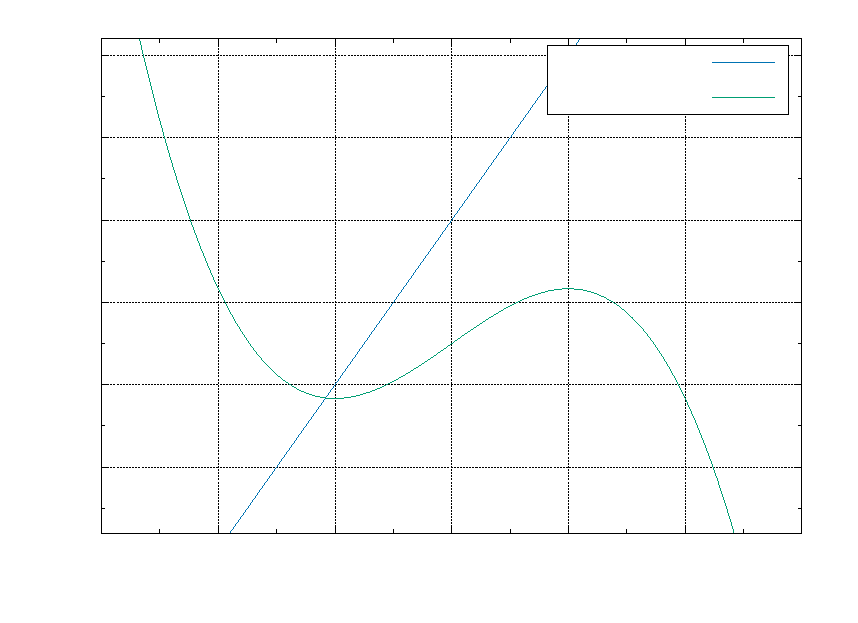
\includegraphics[width={396.80bp},height={283.40bp}]{FHNNullcline}}%
    \gplfronttext
  \end{picture}%
\endgroup

	\caption{Nullcline delle equazioni del modello di FitzHugh-Nagumo.}
\end{figure}
A questo punto studiamo i segni delle derivate, e quindi il campo vettoriali. \\
Se siamo sopra la cubica, la derivata delle $V$ è negativa, mentre questa derivata è positiva sotto alla cubica. La retta invece definisce la derivata della $W$, e tale derivata è negativa sopra alla retta e positiva sotto di essa. In questo modo si divide lo spazio delle fasi in 4 regioni dove i segni delle componenti del campo vettoriale sono diversi, e vediamo che, come per l'oscillatore di Van Der Pol, questo campo ha la funzione di riportare il punto sulla nullclina cubica. \\
Si potrebbe pensare che il punto sia di equilibrio, e per capire se sia veramente così lo studiamo. \\
Definiamo $\delta V = V - V_p$ e $\delta W = W - W_p$, dove il punto di equilibrio è $(V_p,W_p)$. Ora che abbiamo linearizzato il sistema otteniamo il sistema
\begin{equation}
	\begin{cases}
		\delta \dot{V} = (1-V^2_p)\delta V - \delta W \\
		\delta \dot{W} = \frac{1}{\tau}\delta V - \frac{b}{\tau}\delta W 
	\end{cases}
\end{equation}
e così è definita la matrice 
\begin{equation}
	J = \begin{pmatrix}
		(1-V_p^2) & -1 \\
		\frac{1}{\tau} & -\frac{b}{\tau}
	\end{pmatrix}
\end{equation}
Il determinante di questa matrice vale
$$
	det \ J = -\frac{b}{\tau}(1-V_p^2) + \frac{1}{\tau}
$$
Se $V_p$ è grande, il determinante è sempre positivo e il punto è sicuramente stabile. \\
Se però aumento lo stimolo $I$, traslo la cubica verso l'alto, e questo sposta il punto di equilibrio verso l'origine, e così facendo il determinare può diventare negativo. Se a questo punto la traccia diventasse positiva, cambierebbe la stabilità e il punto diventerebbe instabile. Se il punto si sposta poco dal punto di equilibrio, rimane nella zona di stabilità e vi ritorna. Se invece lo stimolo è grande e il punto si sposta molto dall'equilibrio si ottiene una traiettoria molto simile a quella dell'oscillatore di Van Der Pol. \\ 
Questo effetto si dice di pseudo-soglia, perchè le traiettorie nei due casi non sono completamente diversi, bensì si ha una transizione continua tra le due. \\
Per ottenere questo effetto si può usare uno stimolo con la forma di una delta di Dirac
\begin{equation}
	I(t) = \Delta x\delta(t')
\end{equation}
dove $\Delta x$ è l'intensità dello stimolo e $t'$ è il tempo a cui viene somministrato. \\ \\
Questo sistema di equazioni differenziali è un sistema che si dice stiff (verranno approfondite di più le equazioni stiff nella sezione precedente), perchè le due equazioni hanno scale temporali molto diverse, la prima ha scala $1$ mentre la seconda ha scala $1/\tau \ll 1$, quindi è difficile trattarle, perchè essendo messe a sistema devono essere risolte contemporanemente, ma il fatto che evolvano su scale temporali diverse rende difficile scegliere un timestep che sia adeguato per entrambe.  \\ \\
Anche per questo sistema definiamo la funzione di Ljapounov definita in precedenza (che in questo caso indichiamo con $H$ invece che con $V$ per evitare confuzione)
\begin{equation}
	H = \frac{1}{2}\left(W^2 + \frac{V^2}{\tau} \right) 
\end{equation}
che definisce un ellisse. Calcoliamo la derivata temporale di questa funzione
$$
	\frac{dH}{dt} = W\dot{W} + \frac{1}{\tau}V\dot{V} = \frac{W}{\tau}\left(V+a-bW\right)+\frac{1}{\tau}V\left(V - \frac{V^3}{3}-W+I \right) = 
$$
$$
	=\frac{Wa}{\tau} - \frac{bW^2}{\tau} + \frac{V^2}{\tau} - \frac{V^4}{3\tau} + \frac{V}{\tau} < 0
$$
e vediamo che i due termini dominanti, cioè $V^4$ e $W^2$, sono negativi, quindi molto lontano dall'origine il sistema non può espandersi all'infinito. Quello che si trova è una biforcazione di Hopf, ovvero il sistema si espande da un punto fino a che non arriva a un ciclo limite, cioè una traiettoria percorsa che diventa anche attrattiva (e questo fu uno dei primi esempi in cui si vide che oltre ai punti, anche delle intere traiettorie possono essere attrattive). \\
Questo comportamento era caratteristico dell'oscillatore di Van Der Pol e mostra un'ulteriore collegamento tra questi due importanti modelli. \\ \\
Anche in questo caso è possibili accoppiare due neuroni, che si accoppieranno e si stimoleranno a vicenda, autosostenendo le loro traiettorie.
\subsection{Teoria del caos in breve}
Quando si parla di caos si intende una teoria scientifica e matematica che riguarda l'evoluzione temporale di sistemi dinamici altamente sensibili alle condizioni iniziali e la cui evoluzione appare casuale e priva di una legge deterministica sottostante. \\
Secondo la teoria del caos, questi sistemi dinamici in realtà possiedono una legge deterministica che ne governa l'evoluzione, ma risulta molto difficile fare previsioni accurate a partire dalla conoscenza sullo stato attuale del sistema. Data questa difficoltà nel prevederne l'evoluzione, allora appare che tali sistemi evolvano casualmente e senza una legge deterministica.
Tuttavia, poiché (secondo tale teoria) questi sistemi hanno una legge che li governa, allora la loro evoluzione è in realtà determinata a partire dallo stato attuale (ecco perché si parla di caos  deterministico, o semplicemente caos). \\
I sistemi caotici sono sistemi dinamici governati da leggi non lineari e sensibili alle condizioni iniziali: ciò significa che a partire da due condizioni iniziali molto vicine (indicate con $x_0$ e $x_0 + \varepsilon$), le due evoluzioni del sistema nel tempo (indicate con $x(t)$) si discosteranno sempre di più tra loro, a differenza di ciò che accade con sistemi non caotici.
In particolare, ciò che si osserva è che durante una certa scala di tempo le evoluzioni temporali possono essere predette con una certa accuratezza, successivamente iniziano manifestamente a discostarsi e diventare imprevedibili. Tale scala di tempo è legata ad alcuni fattori, come:

1) L'accuratezza con cui possono essere misurate le condizioni sullo stato attuale del sistema. 

2) Il tempo di Lyapunov. \\ 
Il tempo di Lyapunov è una scala di tempo dipendente dalla dinamica del sistema, legato a sua volta all'esponente di Lyapunov $\lambda$, in particolare è definito come $\tau = \lambda_{max}^{-1}$, in cui $\lambda_{max}$ è il massimo esponente di Lyapunov del sistema.

\subsubsection{Esponente di Lyapunov}

\begin{figure}[H]
	\centering
	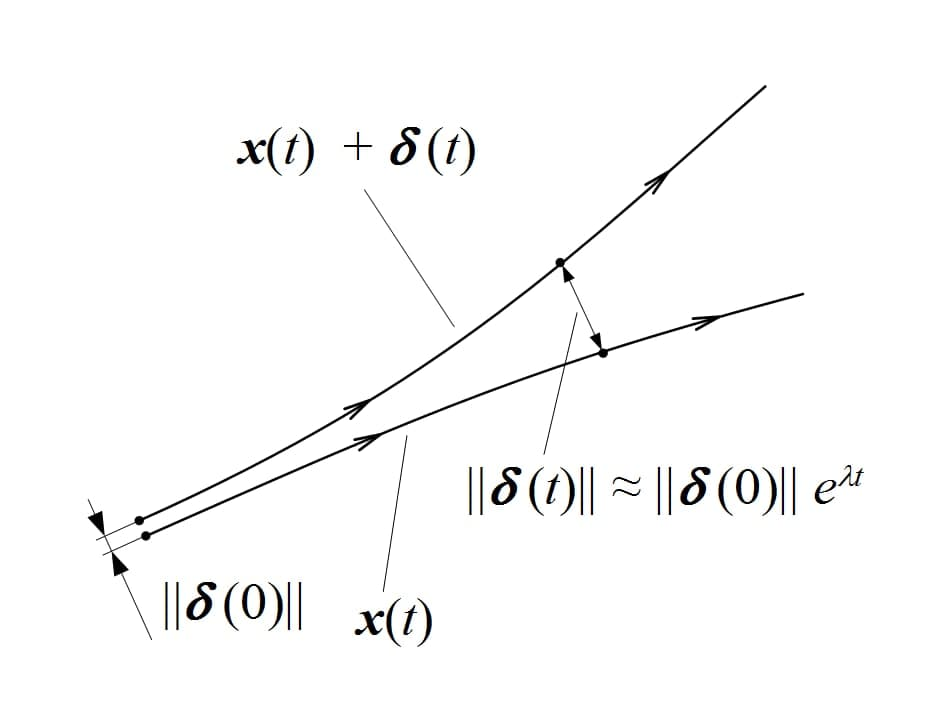
\includegraphics[scale=0.5]{Lyap_Exp}
	\caption{Rappresentazione che mostra il significato dell'esponente di Lyapunov nel contesto dei sistemi caotici.}
\end{figure}

Tale quantità è indice di quanto due traiettorie vicine tendono a discostarsi con l'evolvere del sistema nel tempo, quindi di quanto il sistema è sensibile alle  condizioni  iniziali.
Per quanto detto precedentemente, i sistemi caotici sono molto sensibili alle condizioni iniziali, perciò date due condizioni iniziali arbitrariamente vicine $x_0$ e $x_0 + \delta(0)$, le loro traiettorie $x(t)$ si discosteranno.\\
Si assume generalente che per molti sistemi caotici la distanza tra le traiettorie cresca in maniera esponenziale (si usa l'esponenziale poiché è la più semplice funzione avente un'elevata crescita nel tempo): allora si può definire l'esponente di Lyapunov, essendo $|\delta(t)|$ la distanza tra le traiettorie in funzione del tempo e $|\delta(0)|$ la distanza tra le due condizioni iniziali:
$$
|\delta(t)| \approx |\delta(0)|e^{\lambda t}
$$
Da tale condizione si può ricavare una stima per l'esponente di Lyapunov:
\begin{equation}
	\lambda =\lim_{t\to\infty} \lim_{\delta(0)\to 0} \frac{1}{t}\ln{\frac{|\delta(t)|}{|\delta(0)|}}
\end{equation}
Se si considera un sistema tempo  discreto, in cui l'evoluzione è data da una iterazione $x_{t+1} = f(x_t)$, si può scrivere l'esponente di Lyapunov come legato alla distanza tra l'iterazione al tempo $t$ sulle due diverse condizioni iniziali:
$$
|f^t(x_0 + \delta)-f^t(x_0)| \approx \delta e^{\lambda t}
$$
\begin{equation}
	\lambda =\lim_{t\to\infty} \frac{1}{t}\ln{\left|\frac{df^t}{dx}(x_0)\right|}
\end{equation}

\begin{figure}
	\centering
	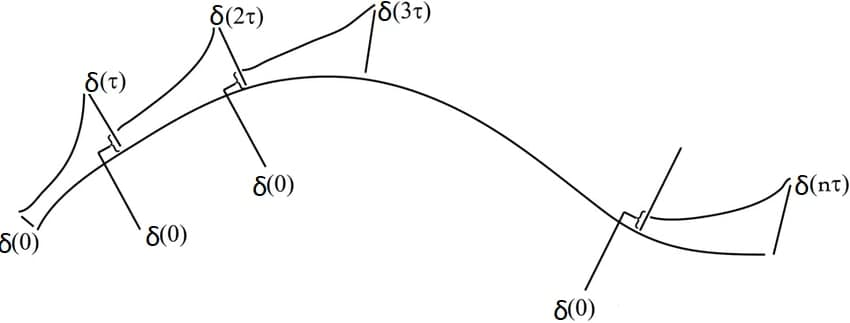
\includegraphics[scale = 0.6]{Lyap_Exp_Calc}
	\caption{Rappresentazione che mostra la procedura utilizzata per la stima numerica dell'esponente di Lyapunov.}
	\label{Ly}
\end{figure}
Se non si ha a disposizione una espressione per la funzione $f(x_t)$ in Eq. 14 si può ricorrere ad una stima dell'esponente di Lyapunov mediante calcolo numerico: la procedura è schematizzata in Fig. \ref{Ly}.
Si parte da due punti nello spazio delle fasi con condizioni iniziali  $x_0$ e $x_1 = x_0 + \delta(0)$ separate da una distanza $\delta(0)$. Questi due punti vengono fatti evolvere per un certo tempo $\tau$, dopo il quale la loro distanza sarà diventata $\delta(\tau))$, dopodiché quest'ultima viene riscalata in modo da reimpostarla al valore iniziale $\delta(0)$ e si procede iterativamente, trovando tanti valori $\delta(n\tau)$. La procedura è iterata fino ad un tempo $t$ (che dovrebbe essere abbastanza grande).
La stima per l'esponente di Lyapunov è allora la seguente media temporale:
\begin{equation}
	\lambda = \frac{1}{t}\sum_{n} \ln\left(\frac{\delta(n \tau)}{\delta(0)}\right)
\end{equation}

L'esponente di Lyapunov è una proprietà dell'orbita del sistema, non del singolo punto, perciò è una proprietà globale. Esso fornisce una stima, come detto precedentemente, di quanto due orbite si discostano a partire da una differenza $\delta(0)$ nelle condizioni iniziali.
Se un sistema ha un esponente di Lyapunov negativo allora significa che due orbite inizialmente  vicine tenderanno ad avvicinarsi sempre di più.
Viceversa, se un sistema ha esponente di Lyapunov positivo allora due orbite tenderanno ad allontanarsi e divergere. Quest'ultima è una condizione che esprime la proprietà di sensitività alle condizioni iniziali di un sistema dinamico ed è una condizione richiesta affinché un sistema sia caotico. \\ \\
Risulta particolarmente importante riflettere sul significato del $\delta(0)$ introdotto: esso rappresenta una differenza numerica tra due possibili condizioni iniziali da cui si suppone inizi l'evoluzione del sistema dinamico oggetto di studio.
Questa differenza può essere pensata come un errore (incertezza sperimentale) nella conoscenza della condizione iniziale da cui si vuole prevedere il futuro dell'evoluzione del sistema.
Da qui emerge l'importanza dell'esponente di Lyapunov nel contesto dei sistemi complessi, poiché fornisce una stima del tempo di predittività del sistema. \\
Si supponga allora di avere un'incertezza $\delta(0)$ sulle condizioni iniziali (fisicamente questa può essere rappresentata da un'incertezza sulla posizione di un corpo in moto, o sulla sua velocità, su una tensione o qualsiasi altra grandezza).
Tale incertezza crescerà quindi esponenzialmente, come precedentemente detto, secondo $\delta(t) \approx \delta(0)e^{(\lambda t)}$. \\
L'incertezza è legata alla predittività del sistema. Il sistema diventerà imprevedibile quando l'incertezza diventerà $O(1)$. \\
Si può allora stimare il \textit{tempo di predittività} come:
$$
\delta(0)e^{\lambda t_p} \approx 1
$$
da cui si esplicita il tempo $t_p$:
\begin{equation}
	t_p = -\frac{\ln(\delta(0))}{\lambda}.
\end{equation}

\subsection{Varianti: L'oscillatore di Van Der Pol forzato}

Una variante dell'oscillatore di Van der Pol è stata studiata (già da Van der Pol stesso): si tratta dell'oscillatore di Van der Pol forzato.
Tale tipologia di oscillatore è governato dalla stessa equazione differenziale vista nella sezione 1.1, a cui è aggiunta una forzante sinusoidale (quindi periodica, di periodo $T_F$ e frequenza $f_F = 1/T_F$).
L'equazione dell'oscillatore forzato diventa quindi:
$$
\ddot{x} - \mu(1-x^2)\dot{x} + x = Acos(2\pi f_F t)
$$
che si può riscrivere come:
\begin{equation}
	\label{EqForced}
	\ddot{x} - \mu(1-x^2)\dot{x} + x - Acos(2\pi f_F t) = 0
\end{equation}
Questa equazione differenziale descrive perciò un oscillatore di Van der Pol che viene stimolato da una forzante esterna, con una certa frequenza $f_F$. \\
Lo studio di tale sistema è molto interessante poiché presenta delle soluzioni caotiche per alcuni valori del parametro $\mu$. \\
Si osserva in Fig. \ref{VDPF} un esempio di soluzione $x(t)$ per l'oscillatore forzato. Si nota un comportamento caotico nella forma della soluzione: con picchi e irregolarità.\\
Storicamente Balthasar Van der Pol ed il suo collega van der Mark furono tra i primi ad osservare questo comportamento tipico del caos deterministico in un circuito elettrico.
Nella sezione 3.1 sono riportati ulteriori approfondimenti, analisi e simulazioni dell'oscillatore di Van der Pol forzato.
\section{Soluzione numerica e simulazione}
Per risolvere l'equazione differenziale dell'oscillatore è stato scritto un codice in C++, che ha permesso di trovare i valori di $x$ per dei valori di tempo discretizzati $t = n\Delta$. Per fare ciò si è partiti dall'equazione 2, ma per permettere al computer di interpretarla la si è dovuta discretizzare, ottenendo il seguente sistema:
\begin{equation}
	\begin{cases}
	x_{n+1} = x_n + y_n\Delta \\
	y_{n+1} = y_n + \left(\mu(1-x_n^2)y_n - x_n\right)\Delta
	\end{cases}
\end{equation} 
Sulla base di questo sistema di equazioni discretizzate è stato scritto il codice presente in appendice. \\
Come di vede, questo codice prende come parametri di entrata le coordinate iniziali $x_0$ e $y_0$, il parametro di smorzamento $\mu$ e lo step temporale $\Delta$. L'ultimo parametro è il tempo $t$, e scegliendo questo valore si ottengono i valori della $x$ per ogni istante temporale precedente al $t$ scelto. \\
	Mediante questo codice vogliamo osservare certe caratteristiche dell'oscillatore: \\
1) Vogliamo osservare la traiettoria caratteristica di un punto nello spazio delle fasi. \\
2) Vogliamo confrontare traiettorie diverse con stesse coordinate iniziali ma con diversi valori del parametro di smorzamento. \\
3) Vogliamo verificare l'attrattivita del ciclo limite. \\
4) Vogliamo infine osservare l'andamento temporale della posizione $x$ della particella. \\
Partiamo dal primo obiettivo, ovvero la traiettoria carattestistica: 
\begin{figure}[H]
	\centering
	\scalebox{0.7}{% GNUPLOT: LaTeX picture with Postscript
\begingroup
  % Encoding inside the plot.  In the header of your document, this encoding
  % should to defined, e.g., by using
  % \usepackage[cp1252,<other encodings>]{inputenc}
  \inputencoding{cp1252}%
  \makeatletter
  \providecommand\color[2][]{%
    \GenericError{(gnuplot) \space\space\space\@spaces}{%
      Package color not loaded in conjunction with
      terminal option `colourtext'%
    }{See the gnuplot documentation for explanation.%
    }{Either use 'blacktext' in gnuplot or load the package
      color.sty in LaTeX.}%
    \renewcommand\color[2][]{}%
  }%
  \providecommand\includegraphics[2][]{%
    \GenericError{(gnuplot) \space\space\space\@spaces}{%
      Package graphicx or graphics not loaded%
    }{See the gnuplot documentation for explanation.%
    }{The gnuplot epslatex terminal needs graphicx.sty or graphics.sty.}%
    \renewcommand\includegraphics[2][]{}%
  }%
  \providecommand\rotatebox[2]{#2}%
  \@ifundefined{ifGPcolor}{%
    \newif\ifGPcolor
    \GPcolortrue
  }{}%
  \@ifundefined{ifGPblacktext}{%
    \newif\ifGPblacktext
    \GPblacktextfalse
  }{}%
  % define a \g@addto@macro without @ in the name:
  \let\gplgaddtomacro\g@addto@macro
  % define empty templates for all commands taking text:
  \gdef\gplbacktext{}%
  \gdef\gplfronttext{}%
  \makeatother
  \ifGPblacktext
    % no textcolor at all
    \def\colorrgb#1{}%
    \def\colorgray#1{}%
  \else
    % gray or color?
    \ifGPcolor
      \def\colorrgb#1{\color[rgb]{#1}}%
      \def\colorgray#1{\color[gray]{#1}}%
      \expandafter\def\csname LTw\endcsname{\color{white}}%
      \expandafter\def\csname LTb\endcsname{\color{black}}%
      \expandafter\def\csname LTa\endcsname{\color{black}}%
      \expandafter\def\csname LT0\endcsname{\color[rgb]{1,0,0}}%
      \expandafter\def\csname LT1\endcsname{\color[rgb]{0,1,0}}%
      \expandafter\def\csname LT2\endcsname{\color[rgb]{0,0,1}}%
      \expandafter\def\csname LT3\endcsname{\color[rgb]{1,0,1}}%
      \expandafter\def\csname LT4\endcsname{\color[rgb]{0,1,1}}%
      \expandafter\def\csname LT5\endcsname{\color[rgb]{1,1,0}}%
      \expandafter\def\csname LT6\endcsname{\color[rgb]{0,0,0}}%
      \expandafter\def\csname LT7\endcsname{\color[rgb]{1,0.3,0}}%
      \expandafter\def\csname LT8\endcsname{\color[rgb]{0.5,0.5,0.5}}%
    \else
      % gray
      \def\colorrgb#1{\color{black}}%
      \def\colorgray#1{\color[gray]{#1}}%
      \expandafter\def\csname LTw\endcsname{\color{white}}%
      \expandafter\def\csname LTb\endcsname{\color{black}}%
      \expandafter\def\csname LTa\endcsname{\color{black}}%
      \expandafter\def\csname LT0\endcsname{\color{black}}%
      \expandafter\def\csname LT1\endcsname{\color{black}}%
      \expandafter\def\csname LT2\endcsname{\color{black}}%
      \expandafter\def\csname LT3\endcsname{\color{black}}%
      \expandafter\def\csname LT4\endcsname{\color{black}}%
      \expandafter\def\csname LT5\endcsname{\color{black}}%
      \expandafter\def\csname LT6\endcsname{\color{black}}%
      \expandafter\def\csname LT7\endcsname{\color{black}}%
      \expandafter\def\csname LT8\endcsname{\color{black}}%
    \fi
  \fi
    \setlength{\unitlength}{0.0500bp}%
    \ifx\gptboxheight\undefined%
      \newlength{\gptboxheight}%
      \newlength{\gptboxwidth}%
      \newsavebox{\gptboxtext}%
    \fi%
    \setlength{\fboxrule}{0.5pt}%
    \setlength{\fboxsep}{1pt}%
    \definecolor{tbcol}{rgb}{1,1,1}%
\begin{picture}(6802.00,6802.00)%
    \gplgaddtomacro\gplbacktext{%
      \csname LTb\endcsname%%
      \put(682,704){\makebox(0,0)[r]{\strut{}$-4$}}%
      \put(682,1439){\makebox(0,0)[r]{\strut{}$-3$}}%
      \put(682,2173){\makebox(0,0)[r]{\strut{}$-2$}}%
      \put(682,2908){\makebox(0,0)[r]{\strut{}$-1$}}%
      \put(682,3643){\makebox(0,0)[r]{\strut{}$0$}}%
      \put(682,4377){\makebox(0,0)[r]{\strut{}$1$}}%
      \put(682,5112){\makebox(0,0)[r]{\strut{}$2$}}%
      \put(682,5846){\makebox(0,0)[r]{\strut{}$3$}}%
      \put(682,6581){\makebox(0,0)[r]{\strut{}$4$}}%
      \put(814,484){\makebox(0,0){\strut{}$-2.5$}}%
      \put(1373,484){\makebox(0,0){\strut{}$-2$}}%
      \put(1932,484){\makebox(0,0){\strut{}$-1.5$}}%
      \put(2491,484){\makebox(0,0){\strut{}$-1$}}%
      \put(3050,484){\makebox(0,0){\strut{}$-0.5$}}%
      \put(3610,484){\makebox(0,0){\strut{}$0$}}%
      \put(4169,484){\makebox(0,0){\strut{}$0.5$}}%
      \put(4728,484){\makebox(0,0){\strut{}$1$}}%
      \put(5287,484){\makebox(0,0){\strut{}$1.5$}}%
      \put(5846,484){\makebox(0,0){\strut{}$2$}}%
      \put(6405,484){\makebox(0,0){\strut{}$2.5$}}%
    }%
    \gplgaddtomacro\gplfronttext{%
      \csname LTb\endcsname%%
      \put(209,3642){\rotatebox{-270}{\makebox(0,0){\strut{}p}}}%
      \put(3609,154){\makebox(0,0){\strut{}x}}%
    }%
    \gplbacktext
    \put(0,0){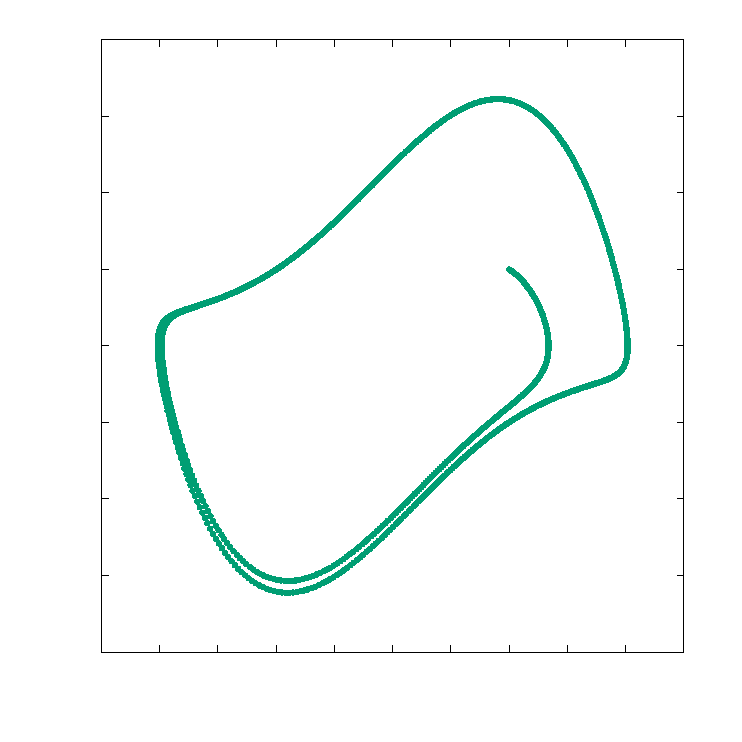
\includegraphics[width={340.10bp},height={340.10bp}]{Schema1-5}}%
    \gplfronttext
  \end{picture}%
\endgroup
}
	\caption{Traiettoria nello spazio delle fasi per $\mu = 1.5$.}
\end{figure}
Nella figura soprastante si può vedere la traiettoria caratteristica dell'oscillatore di Van Der Pol. Come è stato spiegato nelle sezioni precedenti, la velocità del punto che si muove secondo questa traiettoria non è affatto costante.
Come si può notare dall'animazione infatti, il punto si muove molto più velocemente nei lati corti della traiettoria e più lentamente nei lati lunghi. Si avrà quindi un accumulo di punti in corrispondenza dei punti in cui il momento cambia segno,
che nel grafico soprastante si trovano in corrispondenza dei punti $(-2,0)$ e $(2,0)$ approssimativamente. \\
Nell'immagine sottostante si può vedere uno degli ultimi frame dell'animazione citata in precedenza e si vede chiaramente che nei lati corti si hanno degli accumuli di punti, mentre lungo i lati lunghi i punti si distribuiscono in maniera molto meno densa. 
\begin{figure}[H]
	\centering
	\scalebox{0.7}{% GNUPLOT: LaTeX picture with Postscript
\begingroup
  % Encoding inside the plot.  In the header of your document, this encoding
  % should to defined, e.g., by using
  % \usepackage[cp1252,<other encodings>]{inputenc}
  \inputencoding{cp1252}%
  \makeatletter
  \providecommand\color[2][]{%
    \GenericError{(gnuplot) \space\space\space\@spaces}{%
      Package color not loaded in conjunction with
      terminal option `colourtext'%
    }{See the gnuplot documentation for explanation.%
    }{Either use 'blacktext' in gnuplot or load the package
      color.sty in LaTeX.}%
    \renewcommand\color[2][]{}%
  }%
  \providecommand\includegraphics[2][]{%
    \GenericError{(gnuplot) \space\space\space\@spaces}{%
      Package graphicx or graphics not loaded%
    }{See the gnuplot documentation for explanation.%
    }{The gnuplot epslatex terminal needs graphicx.sty or graphics.sty.}%
    \renewcommand\includegraphics[2][]{}%
  }%
  \providecommand\rotatebox[2]{#2}%
  \@ifundefined{ifGPcolor}{%
    \newif\ifGPcolor
    \GPcolortrue
  }{}%
  \@ifundefined{ifGPblacktext}{%
    \newif\ifGPblacktext
    \GPblacktextfalse
  }{}%
  % define a \g@addto@macro without @ in the name:
  \let\gplgaddtomacro\g@addto@macro
  % define empty templates for all commands taking text:
  \gdef\gplbacktext{}%
  \gdef\gplfronttext{}%
  \makeatother
  \ifGPblacktext
    % no textcolor at all
    \def\colorrgb#1{}%
    \def\colorgray#1{}%
  \else
    % gray or color?
    \ifGPcolor
      \def\colorrgb#1{\color[rgb]{#1}}%
      \def\colorgray#1{\color[gray]{#1}}%
      \expandafter\def\csname LTw\endcsname{\color{white}}%
      \expandafter\def\csname LTb\endcsname{\color{black}}%
      \expandafter\def\csname LTa\endcsname{\color{black}}%
      \expandafter\def\csname LT0\endcsname{\color[rgb]{1,0,0}}%
      \expandafter\def\csname LT1\endcsname{\color[rgb]{0,1,0}}%
      \expandafter\def\csname LT2\endcsname{\color[rgb]{0,0,1}}%
      \expandafter\def\csname LT3\endcsname{\color[rgb]{1,0,1}}%
      \expandafter\def\csname LT4\endcsname{\color[rgb]{0,1,1}}%
      \expandafter\def\csname LT5\endcsname{\color[rgb]{1,1,0}}%
      \expandafter\def\csname LT6\endcsname{\color[rgb]{0,0,0}}%
      \expandafter\def\csname LT7\endcsname{\color[rgb]{1,0.3,0}}%
      \expandafter\def\csname LT8\endcsname{\color[rgb]{0.5,0.5,0.5}}%
    \else
      % gray
      \def\colorrgb#1{\color{black}}%
      \def\colorgray#1{\color[gray]{#1}}%
      \expandafter\def\csname LTw\endcsname{\color{white}}%
      \expandafter\def\csname LTb\endcsname{\color{black}}%
      \expandafter\def\csname LTa\endcsname{\color{black}}%
      \expandafter\def\csname LT0\endcsname{\color{black}}%
      \expandafter\def\csname LT1\endcsname{\color{black}}%
      \expandafter\def\csname LT2\endcsname{\color{black}}%
      \expandafter\def\csname LT3\endcsname{\color{black}}%
      \expandafter\def\csname LT4\endcsname{\color{black}}%
      \expandafter\def\csname LT5\endcsname{\color{black}}%
      \expandafter\def\csname LT6\endcsname{\color{black}}%
      \expandafter\def\csname LT7\endcsname{\color{black}}%
      \expandafter\def\csname LT8\endcsname{\color{black}}%
    \fi
  \fi
    \setlength{\unitlength}{0.0500bp}%
    \ifx\gptboxheight\undefined%
      \newlength{\gptboxheight}%
      \newlength{\gptboxwidth}%
      \newsavebox{\gptboxtext}%
    \fi%
    \setlength{\fboxrule}{0.5pt}%
    \setlength{\fboxsep}{1pt}%
    \definecolor{tbcol}{rgb}{1,1,1}%
\begin{picture}(6236.00,6236.00)%
    \gplgaddtomacro\gplbacktext{%
      \csname LTb\endcsname%%
      \put(946,1147){\makebox(0,0)[r]{\strut{}$-2.5$}}%
      \put(946,1589){\makebox(0,0)[r]{\strut{}$-2$}}%
      \put(946,2032){\makebox(0,0)[r]{\strut{}$-1.5$}}%
      \put(946,2474){\makebox(0,0)[r]{\strut{}$-1$}}%
      \put(946,2917){\makebox(0,0)[r]{\strut{}$-0.5$}}%
      \put(946,3360){\makebox(0,0)[r]{\strut{}$0$}}%
      \put(946,3802){\makebox(0,0)[r]{\strut{}$0.5$}}%
      \put(946,4245){\makebox(0,0)[r]{\strut{}$1$}}%
      \put(946,4687){\makebox(0,0)[r]{\strut{}$1.5$}}%
      \put(946,5130){\makebox(0,0)[r]{\strut{}$2$}}%
      \put(946,5572){\makebox(0,0)[r]{\strut{}$2.5$}}%
      \put(1388,484){\makebox(0,0){\strut{}$-2$}}%
      \put(1906,484){\makebox(0,0){\strut{}$-1.5$}}%
      \put(2424,484){\makebox(0,0){\strut{}$-1$}}%
      \put(2941,484){\makebox(0,0){\strut{}$-0.5$}}%
      \put(3459,484){\makebox(0,0){\strut{}$0$}}%
      \put(3976,484){\makebox(0,0){\strut{}$0.5$}}%
      \put(4494,484){\makebox(0,0){\strut{}$1$}}%
      \put(5011,484){\makebox(0,0){\strut{}$1.5$}}%
      \put(5529,484){\makebox(0,0){\strut{}$2$}}%
    }%
    \gplgaddtomacro\gplfronttext{%
      \csname LTb\endcsname%%
      \put(209,3359){\rotatebox{-270}{\makebox(0,0){\strut{}p}}}%
      \put(3458,154){\makebox(0,0){\strut{}x}}%
    }%
    \gplbacktext
    \put(0,0){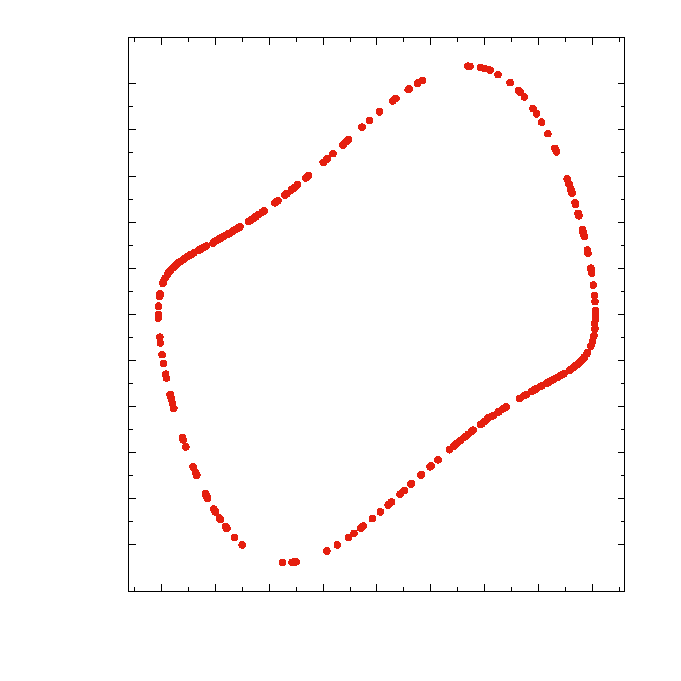
\includegraphics[width={311.80bp},height={311.80bp}]{LastFrame}}%
    \gplfronttext
  \end{picture}%
\endgroup
}
	\caption{Ultimo frame dell'animazione. }
\end{figure}
Vogliamo ora confrontare le traiettorie di particelle aventi stesse coordinate iniziali ma diverse costanti di smorzamento. \\
Ci aspettiamo che il grafico ottenuto dalla simulazione sia simile a quello visto in figura 3. Dalla simulazione si ottiene il seguente grafico: 
\begin{figure}[H]
	\centering
	\scalebox{0.7}{% GNUPLOT: LaTeX picture with Postscript
\begingroup
  % Encoding inside the plot.  In the header of your document, this encoding
  % should to defined, e.g., by using
  % \usepackage[cp1252,<other encodings>]{inputenc}
  \inputencoding{cp1252}%
  \makeatletter
  \providecommand\color[2][]{%
    \GenericError{(gnuplot) \space\space\space\@spaces}{%
      Package color not loaded in conjunction with
      terminal option `colourtext'%
    }{See the gnuplot documentation for explanation.%
    }{Either use 'blacktext' in gnuplot or load the package
      color.sty in LaTeX.}%
    \renewcommand\color[2][]{}%
  }%
  \providecommand\includegraphics[2][]{%
    \GenericError{(gnuplot) \space\space\space\@spaces}{%
      Package graphicx or graphics not loaded%
    }{See the gnuplot documentation for explanation.%
    }{The gnuplot epslatex terminal needs graphicx.sty or graphics.sty.}%
    \renewcommand\includegraphics[2][]{}%
  }%
  \providecommand\rotatebox[2]{#2}%
  \@ifundefined{ifGPcolor}{%
    \newif\ifGPcolor
    \GPcolortrue
  }{}%
  \@ifundefined{ifGPblacktext}{%
    \newif\ifGPblacktext
    \GPblacktextfalse
  }{}%
  % define a \g@addto@macro without @ in the name:
  \let\gplgaddtomacro\g@addto@macro
  % define empty templates for all commands taking text:
  \gdef\gplbacktext{}%
  \gdef\gplfronttext{}%
  \makeatother
  \ifGPblacktext
    % no textcolor at all
    \def\colorrgb#1{}%
    \def\colorgray#1{}%
  \else
    % gray or color?
    \ifGPcolor
      \def\colorrgb#1{\color[rgb]{#1}}%
      \def\colorgray#1{\color[gray]{#1}}%
      \expandafter\def\csname LTw\endcsname{\color{white}}%
      \expandafter\def\csname LTb\endcsname{\color{black}}%
      \expandafter\def\csname LTa\endcsname{\color{black}}%
      \expandafter\def\csname LT0\endcsname{\color[rgb]{1,0,0}}%
      \expandafter\def\csname LT1\endcsname{\color[rgb]{0,1,0}}%
      \expandafter\def\csname LT2\endcsname{\color[rgb]{0,0,1}}%
      \expandafter\def\csname LT3\endcsname{\color[rgb]{1,0,1}}%
      \expandafter\def\csname LT4\endcsname{\color[rgb]{0,1,1}}%
      \expandafter\def\csname LT5\endcsname{\color[rgb]{1,1,0}}%
      \expandafter\def\csname LT6\endcsname{\color[rgb]{0,0,0}}%
      \expandafter\def\csname LT7\endcsname{\color[rgb]{1,0.3,0}}%
      \expandafter\def\csname LT8\endcsname{\color[rgb]{0.5,0.5,0.5}}%
    \else
      % gray
      \def\colorrgb#1{\color{black}}%
      \def\colorgray#1{\color[gray]{#1}}%
      \expandafter\def\csname LTw\endcsname{\color{white}}%
      \expandafter\def\csname LTb\endcsname{\color{black}}%
      \expandafter\def\csname LTa\endcsname{\color{black}}%
      \expandafter\def\csname LT0\endcsname{\color{black}}%
      \expandafter\def\csname LT1\endcsname{\color{black}}%
      \expandafter\def\csname LT2\endcsname{\color{black}}%
      \expandafter\def\csname LT3\endcsname{\color{black}}%
      \expandafter\def\csname LT4\endcsname{\color{black}}%
      \expandafter\def\csname LT5\endcsname{\color{black}}%
      \expandafter\def\csname LT6\endcsname{\color{black}}%
      \expandafter\def\csname LT7\endcsname{\color{black}}%
      \expandafter\def\csname LT8\endcsname{\color{black}}%
    \fi
  \fi
    \setlength{\unitlength}{0.0500bp}%
    \ifx\gptboxheight\undefined%
      \newlength{\gptboxheight}%
      \newlength{\gptboxwidth}%
      \newsavebox{\gptboxtext}%
    \fi%
    \setlength{\fboxrule}{0.5pt}%
    \setlength{\fboxsep}{1pt}%
    \definecolor{tbcol}{rgb}{1,1,1}%
\begin{picture}(5668.00,7370.00)%
    \gplgaddtomacro\gplbacktext{%
      \csname LTb\endcsname%%
      \put(682,704){\makebox(0,0)[r]{\strut{}$-6$}}%
      \put(682,1778){\makebox(0,0)[r]{\strut{}$-4$}}%
      \put(682,2852){\makebox(0,0)[r]{\strut{}$-2$}}%
      \put(682,3927){\makebox(0,0)[r]{\strut{}$0$}}%
      \put(682,5001){\makebox(0,0)[r]{\strut{}$2$}}%
      \put(682,6075){\makebox(0,0)[r]{\strut{}$4$}}%
      \put(682,7149){\makebox(0,0)[r]{\strut{}$6$}}%
      \put(814,484){\makebox(0,0){\strut{}$-2.5$}}%
      \put(1260,484){\makebox(0,0){\strut{}$-2$}}%
      \put(1705,484){\makebox(0,0){\strut{}$-1.5$}}%
      \put(2151,484){\makebox(0,0){\strut{}$-1$}}%
      \put(2597,484){\makebox(0,0){\strut{}$-0.5$}}%
      \put(3043,484){\makebox(0,0){\strut{}$0$}}%
      \put(3488,484){\makebox(0,0){\strut{}$0.5$}}%
      \put(3934,484){\makebox(0,0){\strut{}$1$}}%
      \put(4380,484){\makebox(0,0){\strut{}$1.5$}}%
      \put(4825,484){\makebox(0,0){\strut{}$2$}}%
      \put(5271,484){\makebox(0,0){\strut{}$2.5$}}%
    }%
    \gplgaddtomacro\gplfronttext{%
      \csname LTb\endcsname%%
      \put(209,3926){\rotatebox{-270}{\makebox(0,0){\strut{}p}}}%
      \put(3042,154){\makebox(0,0){\strut{}x}}%
      \csname LTb\endcsname%%
      \put(1738,6921){\makebox(0,0)[r]{\strut{}$\mu = 1$}}%
      \csname LTb\endcsname%%
      \put(1738,6591){\makebox(0,0)[r]{\strut{}$\mu = 2$}}%
      \csname LTb\endcsname%%
      \put(1738,6261){\makebox(0,0)[r]{\strut{}$\mu = 3$}}%
    }%
    \gplbacktext
    \put(0,0){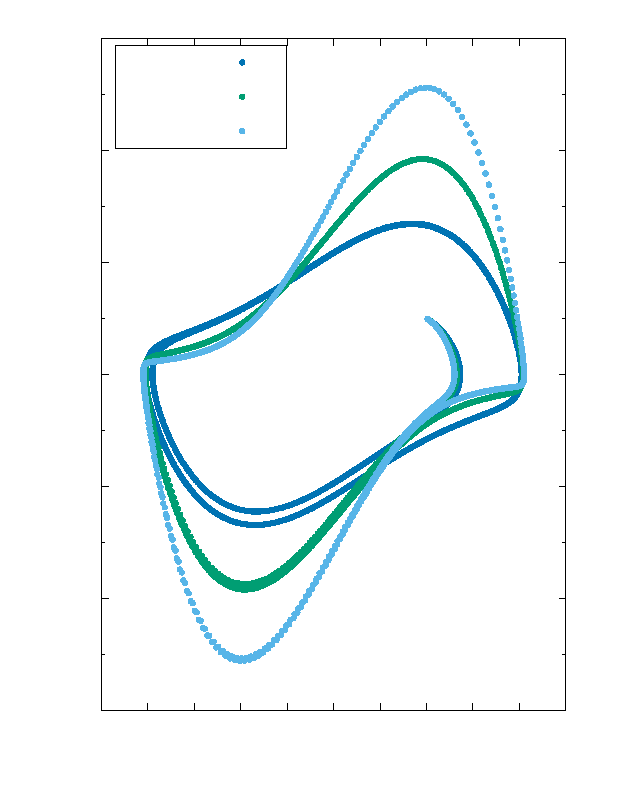
\includegraphics[width={283.40bp},height={368.50bp}]{MuDiversi}}%
    \gplfronttext
  \end{picture}%
\endgroup
}
	\caption{Confronto tra traiettorie con $\mu=1,2,3$.}
\end{figure}
che riporta l'andamento atteso. La cosa principale che si nota è che, con l'aumentare del valore di $\mu$, la traiettoria si allunga e assume una forma pià angolata. Il motivo di questo comportamento è stato spiegato nella sezione precedente e deriva dallo studio dell'equazione differenziale. \\
Vogliamo ora considerare le traiettorie in corrispondenza di valori piccoli di $\mu$. 
\begin{figure}[H]
	\centering
	\scalebox{0.75}{% GNUPLOT: LaTeX picture with Postscript
\begingroup
  % Encoding inside the plot.  In the header of your document, this encoding
  % should to defined, e.g., by using
  % \usepackage[cp1252,<other encodings>]{inputenc}
  \inputencoding{cp1252}%
  \makeatletter
  \providecommand\color[2][]{%
    \GenericError{(gnuplot) \space\space\space\@spaces}{%
      Package color not loaded in conjunction with
      terminal option `colourtext'%
    }{See the gnuplot documentation for explanation.%
    }{Either use 'blacktext' in gnuplot or load the package
      color.sty in LaTeX.}%
    \renewcommand\color[2][]{}%
  }%
  \providecommand\includegraphics[2][]{%
    \GenericError{(gnuplot) \space\space\space\@spaces}{%
      Package graphicx or graphics not loaded%
    }{See the gnuplot documentation for explanation.%
    }{The gnuplot epslatex terminal needs graphicx.sty or graphics.sty.}%
    \renewcommand\includegraphics[2][]{}%
  }%
  \providecommand\rotatebox[2]{#2}%
  \@ifundefined{ifGPcolor}{%
    \newif\ifGPcolor
    \GPcolortrue
  }{}%
  \@ifundefined{ifGPblacktext}{%
    \newif\ifGPblacktext
    \GPblacktextfalse
  }{}%
  % define a \g@addto@macro without @ in the name:
  \let\gplgaddtomacro\g@addto@macro
  % define empty templates for all commands taking text:
  \gdef\gplbacktext{}%
  \gdef\gplfronttext{}%
  \makeatother
  \ifGPblacktext
    % no textcolor at all
    \def\colorrgb#1{}%
    \def\colorgray#1{}%
  \else
    % gray or color?
    \ifGPcolor
      \def\colorrgb#1{\color[rgb]{#1}}%
      \def\colorgray#1{\color[gray]{#1}}%
      \expandafter\def\csname LTw\endcsname{\color{white}}%
      \expandafter\def\csname LTb\endcsname{\color{black}}%
      \expandafter\def\csname LTa\endcsname{\color{black}}%
      \expandafter\def\csname LT0\endcsname{\color[rgb]{1,0,0}}%
      \expandafter\def\csname LT1\endcsname{\color[rgb]{0,1,0}}%
      \expandafter\def\csname LT2\endcsname{\color[rgb]{0,0,1}}%
      \expandafter\def\csname LT3\endcsname{\color[rgb]{1,0,1}}%
      \expandafter\def\csname LT4\endcsname{\color[rgb]{0,1,1}}%
      \expandafter\def\csname LT5\endcsname{\color[rgb]{1,1,0}}%
      \expandafter\def\csname LT6\endcsname{\color[rgb]{0,0,0}}%
      \expandafter\def\csname LT7\endcsname{\color[rgb]{1,0.3,0}}%
      \expandafter\def\csname LT8\endcsname{\color[rgb]{0.5,0.5,0.5}}%
    \else
      % gray
      \def\colorrgb#1{\color{black}}%
      \def\colorgray#1{\color[gray]{#1}}%
      \expandafter\def\csname LTw\endcsname{\color{white}}%
      \expandafter\def\csname LTb\endcsname{\color{black}}%
      \expandafter\def\csname LTa\endcsname{\color{black}}%
      \expandafter\def\csname LT0\endcsname{\color{black}}%
      \expandafter\def\csname LT1\endcsname{\color{black}}%
      \expandafter\def\csname LT2\endcsname{\color{black}}%
      \expandafter\def\csname LT3\endcsname{\color{black}}%
      \expandafter\def\csname LT4\endcsname{\color{black}}%
      \expandafter\def\csname LT5\endcsname{\color{black}}%
      \expandafter\def\csname LT6\endcsname{\color{black}}%
      \expandafter\def\csname LT7\endcsname{\color{black}}%
      \expandafter\def\csname LT8\endcsname{\color{black}}%
    \fi
  \fi
    \setlength{\unitlength}{0.0500bp}%
    \ifx\gptboxheight\undefined%
      \newlength{\gptboxheight}%
      \newlength{\gptboxwidth}%
      \newsavebox{\gptboxtext}%
    \fi%
    \setlength{\fboxrule}{0.5pt}%
    \setlength{\fboxsep}{1pt}%
    \definecolor{tbcol}{rgb}{1,1,1}%
\begin{picture}(6236.00,6236.00)%
    \gplgaddtomacro\gplbacktext{%
      \csname LTb\endcsname%%
      \put(946,704){\makebox(0,0)[r]{\strut{}$-1.5$}}%
      \put(946,1688){\makebox(0,0)[r]{\strut{}$-1$}}%
      \put(946,2671){\makebox(0,0)[r]{\strut{}$-0.5$}}%
      \put(946,3655){\makebox(0,0)[r]{\strut{}$0$}}%
      \put(946,4638){\makebox(0,0)[r]{\strut{}$0.5$}}%
      \put(946,5622){\makebox(0,0)[r]{\strut{}$1$}}%
      \put(1254,484){\makebox(0,0){\strut{}$-1$}}%
      \put(2136,484){\makebox(0,0){\strut{}$-0.5$}}%
      \put(3018,484){\makebox(0,0){\strut{}$0$}}%
      \put(3899,484){\makebox(0,0){\strut{}$0.5$}}%
      \put(4781,484){\makebox(0,0){\strut{}$1$}}%
      \put(5663,484){\makebox(0,0){\strut{}$1.5$}}%
    }%
    \gplgaddtomacro\gplfronttext{%
      \csname LTb\endcsname%%
      \put(209,3359){\rotatebox{-270}{\makebox(0,0){\strut{}p}}}%
      \put(3458,154){\makebox(0,0){\strut{}x}}%
    }%
    \gplbacktext
    \put(0,0){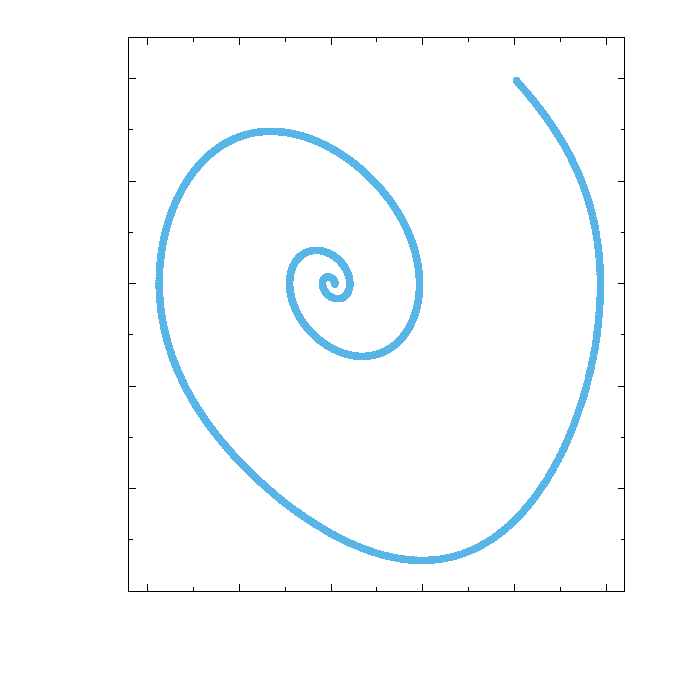
\includegraphics[width={311.80bp},height={311.80bp}]{Collasso}}%
    \gplfronttext
  \end{picture}%
\endgroup
}
	\caption{Traiettoria nello spazio delle fasi per $\mu = -0.5$.}
\end{figure}
Nel grafico soprastante si vede che la particella parte vicino all'origine e viene attratta verso essa, percorrendo quindi delle orbite che degenerano fino a collassare in un punto.
Vogliamo ora studiare l'attrattività del ciclo limite: Consideriamo una situazioni iniziale come quella nel grafico seguente
\begin{figure}[H]
	\centering
	\scalebox{0.75}{% GNUPLOT: LaTeX picture with Postscript
\begingroup
  % Encoding inside the plot.  In the header of your document, this encoding
  % should to defined, e.g., by using
  % \usepackage[cp1252,<other encodings>]{inputenc}
  \inputencoding{cp1252}%
  \makeatletter
  \providecommand\color[2][]{%
    \GenericError{(gnuplot) \space\space\space\@spaces}{%
      Package color not loaded in conjunction with
      terminal option `colourtext'%
    }{See the gnuplot documentation for explanation.%
    }{Either use 'blacktext' in gnuplot or load the package
      color.sty in LaTeX.}%
    \renewcommand\color[2][]{}%
  }%
  \providecommand\includegraphics[2][]{%
    \GenericError{(gnuplot) \space\space\space\@spaces}{%
      Package graphicx or graphics not loaded%
    }{See the gnuplot documentation for explanation.%
    }{The gnuplot epslatex terminal needs graphicx.sty or graphics.sty.}%
    \renewcommand\includegraphics[2][]{}%
  }%
  \providecommand\rotatebox[2]{#2}%
  \@ifundefined{ifGPcolor}{%
    \newif\ifGPcolor
    \GPcolortrue
  }{}%
  \@ifundefined{ifGPblacktext}{%
    \newif\ifGPblacktext
    \GPblacktextfalse
  }{}%
  % define a \g@addto@macro without @ in the name:
  \let\gplgaddtomacro\g@addto@macro
  % define empty templates for all commands taking text:
  \gdef\gplbacktext{}%
  \gdef\gplfronttext{}%
  \makeatother
  \ifGPblacktext
    % no textcolor at all
    \def\colorrgb#1{}%
    \def\colorgray#1{}%
  \else
    % gray or color?
    \ifGPcolor
      \def\colorrgb#1{\color[rgb]{#1}}%
      \def\colorgray#1{\color[gray]{#1}}%
      \expandafter\def\csname LTw\endcsname{\color{white}}%
      \expandafter\def\csname LTb\endcsname{\color{black}}%
      \expandafter\def\csname LTa\endcsname{\color{black}}%
      \expandafter\def\csname LT0\endcsname{\color[rgb]{1,0,0}}%
      \expandafter\def\csname LT1\endcsname{\color[rgb]{0,1,0}}%
      \expandafter\def\csname LT2\endcsname{\color[rgb]{0,0,1}}%
      \expandafter\def\csname LT3\endcsname{\color[rgb]{1,0,1}}%
      \expandafter\def\csname LT4\endcsname{\color[rgb]{0,1,1}}%
      \expandafter\def\csname LT5\endcsname{\color[rgb]{1,1,0}}%
      \expandafter\def\csname LT6\endcsname{\color[rgb]{0,0,0}}%
      \expandafter\def\csname LT7\endcsname{\color[rgb]{1,0.3,0}}%
      \expandafter\def\csname LT8\endcsname{\color[rgb]{0.5,0.5,0.5}}%
    \else
      % gray
      \def\colorrgb#1{\color{black}}%
      \def\colorgray#1{\color[gray]{#1}}%
      \expandafter\def\csname LTw\endcsname{\color{white}}%
      \expandafter\def\csname LTb\endcsname{\color{black}}%
      \expandafter\def\csname LTa\endcsname{\color{black}}%
      \expandafter\def\csname LT0\endcsname{\color{black}}%
      \expandafter\def\csname LT1\endcsname{\color{black}}%
      \expandafter\def\csname LT2\endcsname{\color{black}}%
      \expandafter\def\csname LT3\endcsname{\color{black}}%
      \expandafter\def\csname LT4\endcsname{\color{black}}%
      \expandafter\def\csname LT5\endcsname{\color{black}}%
      \expandafter\def\csname LT6\endcsname{\color{black}}%
      \expandafter\def\csname LT7\endcsname{\color{black}}%
      \expandafter\def\csname LT8\endcsname{\color{black}}%
    \fi
  \fi
    \setlength{\unitlength}{0.0500bp}%
    \ifx\gptboxheight\undefined%
      \newlength{\gptboxheight}%
      \newlength{\gptboxwidth}%
      \newsavebox{\gptboxtext}%
    \fi%
    \setlength{\fboxrule}{0.5pt}%
    \setlength{\fboxsep}{1pt}%
    \definecolor{tbcol}{rgb}{1,1,1}%
\begin{picture}(6236.00,6236.00)%
    \gplgaddtomacro\gplbacktext{%
      \csname LTb\endcsname%%
      \put(946,704){\makebox(0,0)[r]{\strut{}$-2$}}%
      \put(946,1368){\makebox(0,0)[r]{\strut{}$-1.5$}}%
      \put(946,2032){\makebox(0,0)[r]{\strut{}$-1$}}%
      \put(946,2696){\makebox(0,0)[r]{\strut{}$-0.5$}}%
      \put(946,3360){\makebox(0,0)[r]{\strut{}$0$}}%
      \put(946,4023){\makebox(0,0)[r]{\strut{}$0.5$}}%
      \put(946,4687){\makebox(0,0)[r]{\strut{}$1$}}%
      \put(946,5351){\makebox(0,0)[r]{\strut{}$1.5$}}%
      \put(946,6015){\makebox(0,0)[r]{\strut{}$2$}}%
      \put(1078,484){\makebox(0,0){\strut{}$-2$}}%
      \put(1673,484){\makebox(0,0){\strut{}$-1.5$}}%
      \put(2268,484){\makebox(0,0){\strut{}$-1$}}%
      \put(2863,484){\makebox(0,0){\strut{}$-0.5$}}%
      \put(3459,484){\makebox(0,0){\strut{}$0$}}%
      \put(4054,484){\makebox(0,0){\strut{}$0.5$}}%
      \put(4649,484){\makebox(0,0){\strut{}$1$}}%
      \put(5244,484){\makebox(0,0){\strut{}$1.5$}}%
      \put(5839,484){\makebox(0,0){\strut{}$2$}}%
    }%
    \gplgaddtomacro\gplfronttext{%
      \csname LTb\endcsname%%
      \put(209,3359){\rotatebox{-270}{\makebox(0,0){\strut{}p}}}%
      \put(3458,154){\makebox(0,0){\strut{}x}}%
    }%
    \gplbacktext
    \put(0,0){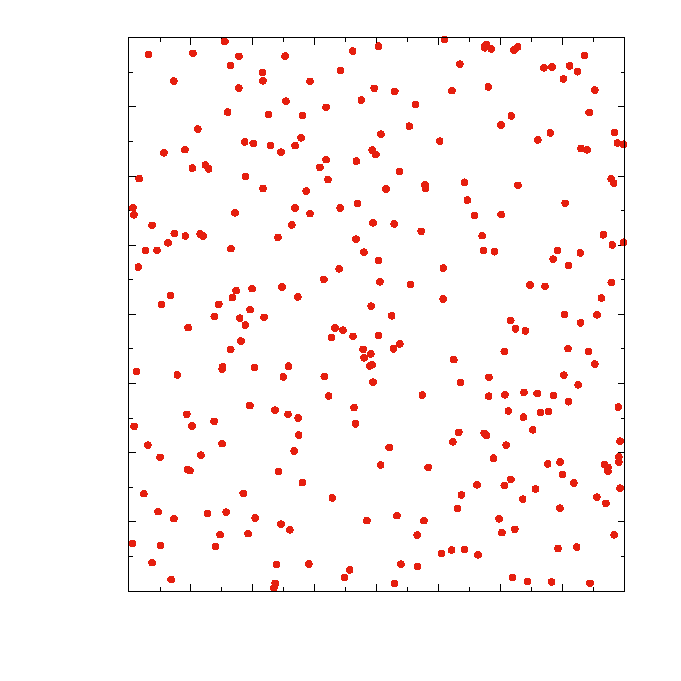
\includegraphics[width={311.80bp},height={311.80bp}]{FirstFrame}}%
    \gplfronttext
  \end{picture}%
\endgroup
}
	\caption{Primo frame dell'animazione.}
\end{figure}
quindi una situazione in cui abbiamo un grande numero di punti (in questo caso ne sono stati plottati 300) che sono distribuiti randomicamente nello spazio delle fasi, quindi con momento iniziale e coordinata $x$ iniziale randomici. \\
Se lasciamo partire questi punti, sembra inizialmente che questi si muovano in modo caotico, ma dopo una decina di iterazioni si vede che le particelle stanno in realtà andando a formare una stessa traiettoria, che è la traiettoria caratteristica dell'oscillatore di Van Der Pol. \\
In base alla loro posizione iniziale i punti ci metteranno più o meno tempo a posizionarsi su questa curva, ma dopo un numero sufficientemente grande di iterazioni (nella simulazione considerata sono servite circa 350 iterazioni) tutti i punti si saranno posizionati sulla curva. \\
Questo comportamento peculiare è un'altra dimostrazione del fatto che la traiettoria dell'oscillatore di Van Der Pol sia una curva attrattiva. \\ \\
Infine si vuole studiare l'andamento temporale della $x$. 
\begin{figure}[H]
	% GNUPLOT: LaTeX picture with Postscript
\begingroup
  % Encoding inside the plot.  In the header of your document, this encoding
  % should to defined, e.g., by using
  % \usepackage[cp1252,<other encodings>]{inputenc}
  \inputencoding{cp1252}%
  \makeatletter
  \providecommand\color[2][]{%
    \GenericError{(gnuplot) \space\space\space\@spaces}{%
      Package color not loaded in conjunction with
      terminal option `colourtext'%
    }{See the gnuplot documentation for explanation.%
    }{Either use 'blacktext' in gnuplot or load the package
      color.sty in LaTeX.}%
    \renewcommand\color[2][]{}%
  }%
  \providecommand\includegraphics[2][]{%
    \GenericError{(gnuplot) \space\space\space\@spaces}{%
      Package graphicx or graphics not loaded%
    }{See the gnuplot documentation for explanation.%
    }{The gnuplot epslatex terminal needs graphicx.sty or graphics.sty.}%
    \renewcommand\includegraphics[2][]{}%
  }%
  \providecommand\rotatebox[2]{#2}%
  \@ifundefined{ifGPcolor}{%
    \newif\ifGPcolor
    \GPcolortrue
  }{}%
  \@ifundefined{ifGPblacktext}{%
    \newif\ifGPblacktext
    \GPblacktextfalse
  }{}%
  % define a \g@addto@macro without @ in the name:
  \let\gplgaddtomacro\g@addto@macro
  % define empty templates for all commands taking text:
  \gdef\gplbacktext{}%
  \gdef\gplfronttext{}%
  \makeatother
  \ifGPblacktext
    % no textcolor at all
    \def\colorrgb#1{}%
    \def\colorgray#1{}%
  \else
    % gray or color?
    \ifGPcolor
      \def\colorrgb#1{\color[rgb]{#1}}%
      \def\colorgray#1{\color[gray]{#1}}%
      \expandafter\def\csname LTw\endcsname{\color{white}}%
      \expandafter\def\csname LTb\endcsname{\color{black}}%
      \expandafter\def\csname LTa\endcsname{\color{black}}%
      \expandafter\def\csname LT0\endcsname{\color[rgb]{1,0,0}}%
      \expandafter\def\csname LT1\endcsname{\color[rgb]{0,1,0}}%
      \expandafter\def\csname LT2\endcsname{\color[rgb]{0,0,1}}%
      \expandafter\def\csname LT3\endcsname{\color[rgb]{1,0,1}}%
      \expandafter\def\csname LT4\endcsname{\color[rgb]{0,1,1}}%
      \expandafter\def\csname LT5\endcsname{\color[rgb]{1,1,0}}%
      \expandafter\def\csname LT6\endcsname{\color[rgb]{0,0,0}}%
      \expandafter\def\csname LT7\endcsname{\color[rgb]{1,0.3,0}}%
      \expandafter\def\csname LT8\endcsname{\color[rgb]{0.5,0.5,0.5}}%
    \else
      % gray
      \def\colorrgb#1{\color{black}}%
      \def\colorgray#1{\color[gray]{#1}}%
      \expandafter\def\csname LTw\endcsname{\color{white}}%
      \expandafter\def\csname LTb\endcsname{\color{black}}%
      \expandafter\def\csname LTa\endcsname{\color{black}}%
      \expandafter\def\csname LT0\endcsname{\color{black}}%
      \expandafter\def\csname LT1\endcsname{\color{black}}%
      \expandafter\def\csname LT2\endcsname{\color{black}}%
      \expandafter\def\csname LT3\endcsname{\color{black}}%
      \expandafter\def\csname LT4\endcsname{\color{black}}%
      \expandafter\def\csname LT5\endcsname{\color{black}}%
      \expandafter\def\csname LT6\endcsname{\color{black}}%
      \expandafter\def\csname LT7\endcsname{\color{black}}%
      \expandafter\def\csname LT8\endcsname{\color{black}}%
    \fi
  \fi
    \setlength{\unitlength}{0.0500bp}%
    \ifx\gptboxheight\undefined%
      \newlength{\gptboxheight}%
      \newlength{\gptboxwidth}%
      \newsavebox{\gptboxtext}%
    \fi%
    \setlength{\fboxrule}{0.5pt}%
    \setlength{\fboxsep}{1pt}%
    \definecolor{tbcol}{rgb}{1,1,1}%
\begin{picture}(10204.00,5668.00)%
    \gplgaddtomacro\gplbacktext{%
      \csname LTb\endcsname%%
      \put(946,704){\makebox(0,0)[r]{\strut{}$-2.5$}}%
      \put(946,1178){\makebox(0,0)[r]{\strut{}$-2$}}%
      \put(946,1653){\makebox(0,0)[r]{\strut{}$-1.5$}}%
      \put(946,2127){\makebox(0,0)[r]{\strut{}$-1$}}%
      \put(946,2601){\makebox(0,0)[r]{\strut{}$-0.5$}}%
      \put(946,3076){\makebox(0,0)[r]{\strut{}$0$}}%
      \put(946,3550){\makebox(0,0)[r]{\strut{}$0.5$}}%
      \put(946,4024){\makebox(0,0)[r]{\strut{}$1$}}%
      \put(946,4498){\makebox(0,0)[r]{\strut{}$1.5$}}%
      \put(946,4973){\makebox(0,0)[r]{\strut{}$2$}}%
      \put(946,5447){\makebox(0,0)[r]{\strut{}$2.5$}}%
      \put(1078,484){\makebox(0,0){\strut{}$0$}}%
      \put(2325,484){\makebox(0,0){\strut{}$5$}}%
      \put(3572,484){\makebox(0,0){\strut{}$10$}}%
      \put(4819,484){\makebox(0,0){\strut{}$15$}}%
      \put(6066,484){\makebox(0,0){\strut{}$20$}}%
      \put(7313,484){\makebox(0,0){\strut{}$25$}}%
      \put(8560,484){\makebox(0,0){\strut{}$30$}}%
      \put(9807,484){\makebox(0,0){\strut{}$35$}}%
    }%
    \gplgaddtomacro\gplfronttext{%
      \csname LTb\endcsname%%
      \put(209,3075){\rotatebox{-270}{\makebox(0,0){\strut{}x(t)}}}%
      \put(5442,154){\makebox(0,0){\strut{}t}}%
      \csname LTb\endcsname%%
      \put(3718,5219){\makebox(0,0)[r]{\strut{}Andamento temporale}}%
    }%
    \gplbacktext
    \put(0,0){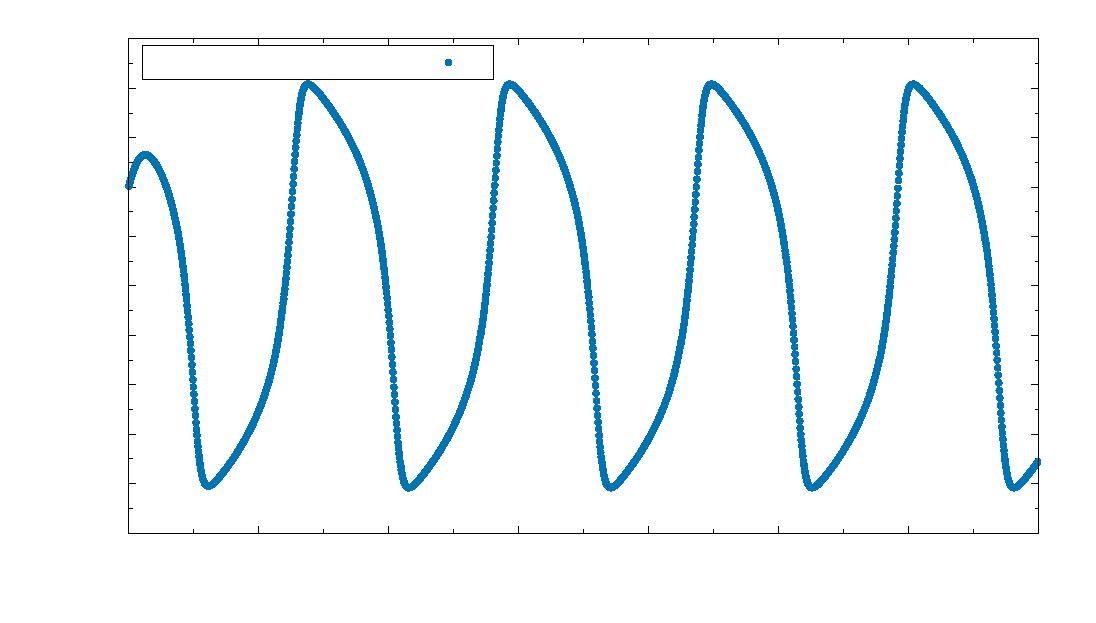
\includegraphics[width={510.20bp},height={283.40bp}]{AndTemp}}%
    \gplfronttext
  \end{picture}%
\endgroup

	\caption{Andamento temporale della $x(t).$}
\end{figure}
Nella figura soprastante si vede che l'andamento della $x$ ricorda vagamente una sinusoide, per la periodicità, ma ha una forma molto più aguzza. Si nota inoltre che la forma della funzione tra un punto di minimo e un punto di massimo e viceverda mantiene la stessa forma, ma risulta capovolta. \\
Si nota inoltre che la forma della funzione tra un punto di minimo e un punto di massimo e viceverda mantiene la stessa forma, ma risulta capovolta. \\
La forma di queste oscillazioni cambia molto con il valore della costante di smorzamento. Infatti si trova che per valori più piccoli di $\mu$ le oscillazioni hanno una forma più aguzza, mentre per valori grandi (da circa 5 in su) l'andamento ha una forma più squadrata. \\
Per rendere l'idea in un modo tutt'altro che rigoroso, per valori piccoli di $\mu$ l'andamento ha una forma che ricorda il dente di un lupo, mentre per valori grandi ha una forma che ricorda il dente di uno squalo. \\ \\ 
Questo è l'andamento temporale nel caso dell'oscillatore non forzato. \\
Per un oscillatore forzato si troverebbe un andamento vagamente simile a questo, ma con una forma molto più irregolare. Questo è dovuto al fatto che in un'oscillatore del genere, una forzante periodica producerebbe una caoticità, che renderebbe quindi molto più imprevedibile la traiettoria.
\subsection{Simulazione dell'oscillatore forzato}
Come per la versione standard, sono state eseguite simulazioni anche per l'oscillatore di Van der Pol forzato. Innanzitutto è stata risolta l'equazione differenziale (Eq. \ref{EqForced}) mediante lo stesso metodo utilizzato precedentemente (e quindi anche lo stesso codice C++).
Si è ottenuto il sistema discretizzando il tempo:
\begin{equation}
	\begin{cases}
		x_{n+1} = x_n + y_n\Delta \\
		y_{n+1} = y_n + \left( \mu(1-x_n^2)y_n-x_n+A\cos(2\pi f_F)\right) \Delta
	\end{cases}
\end{equation}
Tramite il programma scritto sono state risolte alcune equazioni differenziali per osservare il comportamento dell'oscillatore forzato nei diversi regimi.
Nelle simulazioni sono stati assunti i seguenti valori dei parametri (in unità di misura arbitrarie): $f_F = 0.1$, quindi $T_F = 10$, $A = 1.2$ e sono stati osservati diversi regimi a seconda del valore di $\mu$, ossia il parametro che regola la nonlinearità del sistema. \\
Si è osservato, in particolare, che per bassi valori di $\mu$ il sistema si comporta in modo regolare, mentre per alti valori di $\mu$ si osservano regimi caotici e alta sensibilità alle condizioni iniziali.
\begin{figure}[H]
	\centering
	% GNUPLOT: LaTeX picture with Postscript
\begingroup
  % Encoding inside the plot.  In the header of your document, this encoding
  % should to defined, e.g., by using
  % \usepackage[cp1252,<other encodings>]{inputenc}
  \inputencoding{cp1252}%
  \makeatletter
  \providecommand\color[2][]{%
    \GenericError{(gnuplot) \space\space\space\@spaces}{%
      Package color not loaded in conjunction with
      terminal option `colourtext'%
    }{See the gnuplot documentation for explanation.%
    }{Either use 'blacktext' in gnuplot or load the package
      color.sty in LaTeX.}%
    \renewcommand\color[2][]{}%
  }%
  \providecommand\includegraphics[2][]{%
    \GenericError{(gnuplot) \space\space\space\@spaces}{%
      Package graphicx or graphics not loaded%
    }{See the gnuplot documentation for explanation.%
    }{The gnuplot epslatex terminal needs graphicx.sty or graphics.sty.}%
    \renewcommand\includegraphics[2][]{}%
  }%
  \providecommand\rotatebox[2]{#2}%
  \@ifundefined{ifGPcolor}{%
    \newif\ifGPcolor
    \GPcolortrue
  }{}%
  \@ifundefined{ifGPblacktext}{%
    \newif\ifGPblacktext
    \GPblacktextfalse
  }{}%
  % define a \g@addto@macro without @ in the name:
  \let\gplgaddtomacro\g@addto@macro
  % define empty templates for all commands taking text:
  \gdef\gplbacktext{}%
  \gdef\gplfronttext{}%
  \makeatother
  \ifGPblacktext
    % no textcolor at all
    \def\colorrgb#1{}%
    \def\colorgray#1{}%
  \else
    % gray or color?
    \ifGPcolor
      \def\colorrgb#1{\color[rgb]{#1}}%
      \def\colorgray#1{\color[gray]{#1}}%
      \expandafter\def\csname LTw\endcsname{\color{white}}%
      \expandafter\def\csname LTb\endcsname{\color{black}}%
      \expandafter\def\csname LTa\endcsname{\color{black}}%
      \expandafter\def\csname LT0\endcsname{\color[rgb]{1,0,0}}%
      \expandafter\def\csname LT1\endcsname{\color[rgb]{0,1,0}}%
      \expandafter\def\csname LT2\endcsname{\color[rgb]{0,0,1}}%
      \expandafter\def\csname LT3\endcsname{\color[rgb]{1,0,1}}%
      \expandafter\def\csname LT4\endcsname{\color[rgb]{0,1,1}}%
      \expandafter\def\csname LT5\endcsname{\color[rgb]{1,1,0}}%
      \expandafter\def\csname LT6\endcsname{\color[rgb]{0,0,0}}%
      \expandafter\def\csname LT7\endcsname{\color[rgb]{1,0.3,0}}%
      \expandafter\def\csname LT8\endcsname{\color[rgb]{0.5,0.5,0.5}}%
    \else
      % gray
      \def\colorrgb#1{\color{black}}%
      \def\colorgray#1{\color[gray]{#1}}%
      \expandafter\def\csname LTw\endcsname{\color{white}}%
      \expandafter\def\csname LTb\endcsname{\color{black}}%
      \expandafter\def\csname LTa\endcsname{\color{black}}%
      \expandafter\def\csname LT0\endcsname{\color{black}}%
      \expandafter\def\csname LT1\endcsname{\color{black}}%
      \expandafter\def\csname LT2\endcsname{\color{black}}%
      \expandafter\def\csname LT3\endcsname{\color{black}}%
      \expandafter\def\csname LT4\endcsname{\color{black}}%
      \expandafter\def\csname LT5\endcsname{\color{black}}%
      \expandafter\def\csname LT6\endcsname{\color{black}}%
      \expandafter\def\csname LT7\endcsname{\color{black}}%
      \expandafter\def\csname LT8\endcsname{\color{black}}%
    \fi
  \fi
    \setlength{\unitlength}{0.0500bp}%
    \ifx\gptboxheight\undefined%
      \newlength{\gptboxheight}%
      \newlength{\gptboxwidth}%
      \newsavebox{\gptboxtext}%
    \fi%
    \setlength{\fboxrule}{0.5pt}%
    \setlength{\fboxsep}{1pt}%
    \definecolor{tbcol}{rgb}{1,1,1}%
\begin{picture}(10204.00,5668.00)%
    \gplgaddtomacro\gplbacktext{%
      \csname LTb\endcsname%%
      \put(682,1178){\makebox(0,0)[r]{\strut{}$-2$}}%
      \put(682,2127){\makebox(0,0)[r]{\strut{}$-1$}}%
      \put(682,3076){\makebox(0,0)[r]{\strut{}$0$}}%
      \put(682,4024){\makebox(0,0)[r]{\strut{}$1$}}%
      \put(682,4973){\makebox(0,0)[r]{\strut{}$2$}}%
      \put(814,484){\makebox(0,0){\strut{}$0$}}%
      \put(1456,484){\makebox(0,0){\strut{}$5$}}%
      \put(2099,484){\makebox(0,0){\strut{}$10$}}%
      \put(2741,484){\makebox(0,0){\strut{}$15$}}%
      \put(3383,484){\makebox(0,0){\strut{}$20$}}%
      \put(4026,484){\makebox(0,0){\strut{}$25$}}%
      \put(4668,484){\makebox(0,0){\strut{}$30$}}%
      \put(5311,484){\makebox(0,0){\strut{}$35$}}%
      \put(5953,484){\makebox(0,0){\strut{}$40$}}%
      \put(6595,484){\makebox(0,0){\strut{}$45$}}%
      \put(7238,484){\makebox(0,0){\strut{}$50$}}%
      \put(7880,484){\makebox(0,0){\strut{}$55$}}%
      \put(8522,484){\makebox(0,0){\strut{}$60$}}%
      \put(9165,484){\makebox(0,0){\strut{}$65$}}%
      \put(9807,484){\makebox(0,0){\strut{}$70$}}%
    }%
    \gplgaddtomacro\gplfronttext{%
      \csname LTb\endcsname%%
      \put(209,3075){\rotatebox{-270}{\makebox(0,0){\strut{}x(t)}}}%
      \put(5310,154){\makebox(0,0){\strut{}t}}%
    }%
    \gplbacktext
    \put(0,0){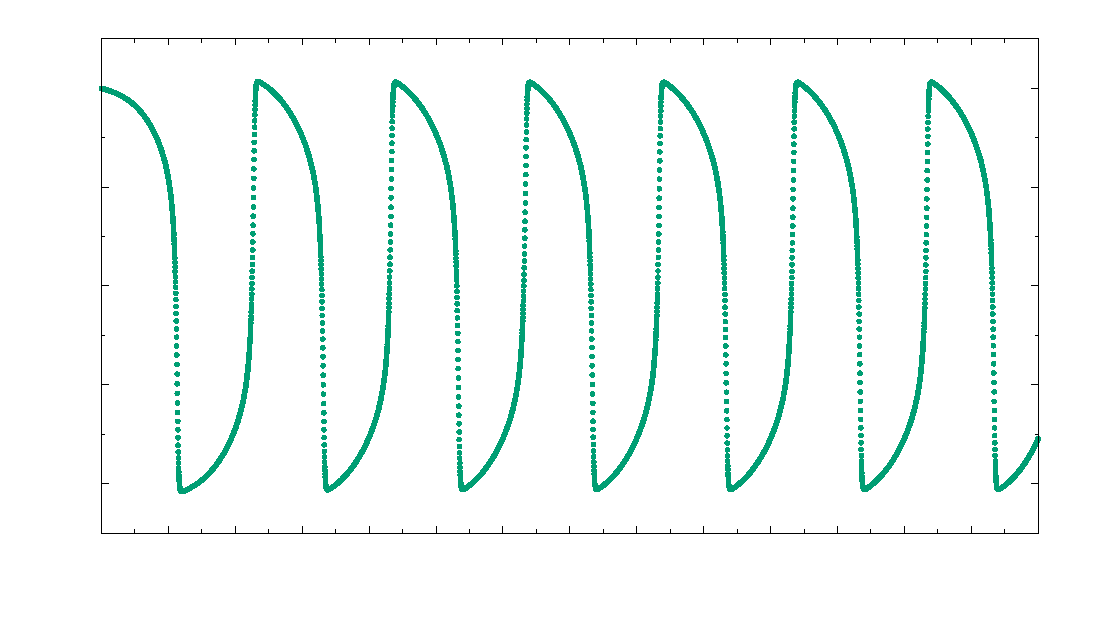
\includegraphics[width={510.20bp},height={283.40bp}]{Caotico4}}%
    \gplfronttext
  \end{picture}%
\endgroup

	\caption{Oscillatore di Van der Pol forzato con $f_F = 0.1$, $A = 1.2$ e $\mu = 6$.}
	\label{VDPF6}
\end{figure}
\begin{figure}[H]
	\centering
	% GNUPLOT: LaTeX picture with Postscript
\begingroup
  % Encoding inside the plot.  In the header of your document, this encoding
  % should to defined, e.g., by using
  % \usepackage[cp1252,<other encodings>]{inputenc}
  \inputencoding{cp1252}%
  \makeatletter
  \providecommand\color[2][]{%
    \GenericError{(gnuplot) \space\space\space\@spaces}{%
      Package color not loaded in conjunction with
      terminal option `colourtext'%
    }{See the gnuplot documentation for explanation.%
    }{Either use 'blacktext' in gnuplot or load the package
      color.sty in LaTeX.}%
    \renewcommand\color[2][]{}%
  }%
  \providecommand\includegraphics[2][]{%
    \GenericError{(gnuplot) \space\space\space\@spaces}{%
      Package graphicx or graphics not loaded%
    }{See the gnuplot documentation for explanation.%
    }{The gnuplot epslatex terminal needs graphicx.sty or graphics.sty.}%
    \renewcommand\includegraphics[2][]{}%
  }%
  \providecommand\rotatebox[2]{#2}%
  \@ifundefined{ifGPcolor}{%
    \newif\ifGPcolor
    \GPcolortrue
  }{}%
  \@ifundefined{ifGPblacktext}{%
    \newif\ifGPblacktext
    \GPblacktextfalse
  }{}%
  % define a \g@addto@macro without @ in the name:
  \let\gplgaddtomacro\g@addto@macro
  % define empty templates for all commands taking text:
  \gdef\gplbacktext{}%
  \gdef\gplfronttext{}%
  \makeatother
  \ifGPblacktext
    % no textcolor at all
    \def\colorrgb#1{}%
    \def\colorgray#1{}%
  \else
    % gray or color?
    \ifGPcolor
      \def\colorrgb#1{\color[rgb]{#1}}%
      \def\colorgray#1{\color[gray]{#1}}%
      \expandafter\def\csname LTw\endcsname{\color{white}}%
      \expandafter\def\csname LTb\endcsname{\color{black}}%
      \expandafter\def\csname LTa\endcsname{\color{black}}%
      \expandafter\def\csname LT0\endcsname{\color[rgb]{1,0,0}}%
      \expandafter\def\csname LT1\endcsname{\color[rgb]{0,1,0}}%
      \expandafter\def\csname LT2\endcsname{\color[rgb]{0,0,1}}%
      \expandafter\def\csname LT3\endcsname{\color[rgb]{1,0,1}}%
      \expandafter\def\csname LT4\endcsname{\color[rgb]{0,1,1}}%
      \expandafter\def\csname LT5\endcsname{\color[rgb]{1,1,0}}%
      \expandafter\def\csname LT6\endcsname{\color[rgb]{0,0,0}}%
      \expandafter\def\csname LT7\endcsname{\color[rgb]{1,0.3,0}}%
      \expandafter\def\csname LT8\endcsname{\color[rgb]{0.5,0.5,0.5}}%
    \else
      % gray
      \def\colorrgb#1{\color{black}}%
      \def\colorgray#1{\color[gray]{#1}}%
      \expandafter\def\csname LTw\endcsname{\color{white}}%
      \expandafter\def\csname LTb\endcsname{\color{black}}%
      \expandafter\def\csname LTa\endcsname{\color{black}}%
      \expandafter\def\csname LT0\endcsname{\color{black}}%
      \expandafter\def\csname LT1\endcsname{\color{black}}%
      \expandafter\def\csname LT2\endcsname{\color{black}}%
      \expandafter\def\csname LT3\endcsname{\color{black}}%
      \expandafter\def\csname LT4\endcsname{\color{black}}%
      \expandafter\def\csname LT5\endcsname{\color{black}}%
      \expandafter\def\csname LT6\endcsname{\color{black}}%
      \expandafter\def\csname LT7\endcsname{\color{black}}%
      \expandafter\def\csname LT8\endcsname{\color{black}}%
    \fi
  \fi
    \setlength{\unitlength}{0.0500bp}%
    \ifx\gptboxheight\undefined%
      \newlength{\gptboxheight}%
      \newlength{\gptboxwidth}%
      \newsavebox{\gptboxtext}%
    \fi%
    \setlength{\fboxrule}{0.5pt}%
    \setlength{\fboxsep}{1pt}%
    \definecolor{tbcol}{rgb}{1,1,1}%
\begin{picture}(10204.00,5668.00)%
    \gplgaddtomacro\gplbacktext{%
      \csname LTb\endcsname%%
      \put(946,704){\makebox(0,0)[r]{\strut{}$-2.5$}}%
      \put(946,1178){\makebox(0,0)[r]{\strut{}$-2$}}%
      \put(946,1653){\makebox(0,0)[r]{\strut{}$-1.5$}}%
      \put(946,2127){\makebox(0,0)[r]{\strut{}$-1$}}%
      \put(946,2601){\makebox(0,0)[r]{\strut{}$-0.5$}}%
      \put(946,3076){\makebox(0,0)[r]{\strut{}$0$}}%
      \put(946,3550){\makebox(0,0)[r]{\strut{}$0.5$}}%
      \put(946,4024){\makebox(0,0)[r]{\strut{}$1$}}%
      \put(946,4498){\makebox(0,0)[r]{\strut{}$1.5$}}%
      \put(946,4973){\makebox(0,0)[r]{\strut{}$2$}}%
      \put(946,5447){\makebox(0,0)[r]{\strut{}$2.5$}}%
      \put(1078,484){\makebox(0,0){\strut{}$0$}}%
      \put(1514,484){\makebox(0,0){\strut{}$5$}}%
      \put(1951,484){\makebox(0,0){\strut{}$10$}}%
      \put(2387,484){\makebox(0,0){\strut{}$15$}}%
      \put(2824,484){\makebox(0,0){\strut{}$20$}}%
      \put(3260,484){\makebox(0,0){\strut{}$25$}}%
      \put(3697,484){\makebox(0,0){\strut{}$30$}}%
      \put(4133,484){\makebox(0,0){\strut{}$35$}}%
      \put(4570,484){\makebox(0,0){\strut{}$40$}}%
      \put(5006,484){\makebox(0,0){\strut{}$45$}}%
      \put(5443,484){\makebox(0,0){\strut{}$50$}}%
      \put(5879,484){\makebox(0,0){\strut{}$55$}}%
      \put(6315,484){\makebox(0,0){\strut{}$60$}}%
      \put(6752,484){\makebox(0,0){\strut{}$65$}}%
      \put(7188,484){\makebox(0,0){\strut{}$70$}}%
      \put(7625,484){\makebox(0,0){\strut{}$75$}}%
      \put(8061,484){\makebox(0,0){\strut{}$80$}}%
      \put(8498,484){\makebox(0,0){\strut{}$85$}}%
      \put(8934,484){\makebox(0,0){\strut{}$90$}}%
      \put(9371,484){\makebox(0,0){\strut{}$95$}}%
      \put(9807,484){\makebox(0,0){\strut{}$100$}}%
    }%
    \gplgaddtomacro\gplfronttext{%
      \csname LTb\endcsname%%
      \put(209,3075){\rotatebox{-270}{\makebox(0,0){\strut{}x(t)}}}%
      \put(5442,154){\makebox(0,0){\strut{}t}}%
    }%
    \gplbacktext
    \put(0,0){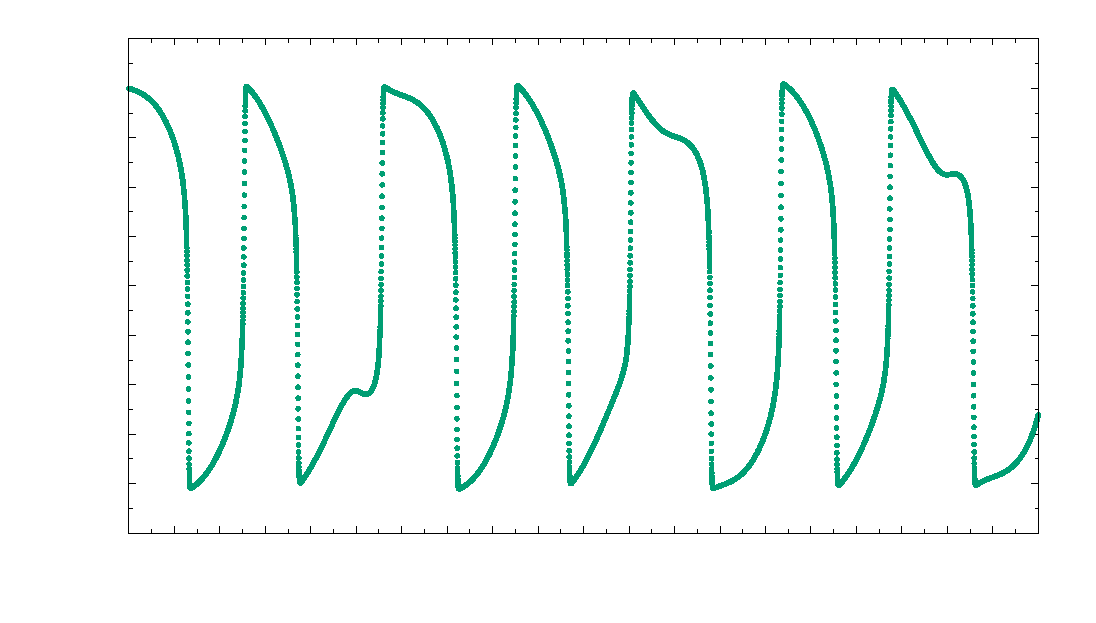
\includegraphics[width={510.20bp},height={283.40bp}]{Caotico2}}%
    \gplfronttext
  \end{picture}%
\endgroup

	\caption{Oscillatore di Van der Pol forzato con $f_F = 0.1$, $A = 1.2$ e $\mu = 8$.}
	\label{VDPF8}
\end{figure}
\begin{figure}[H]
	\centering
	% GNUPLOT: LaTeX picture with Postscript
\begingroup
  % Encoding inside the plot.  In the header of your document, this encoding
  % should to defined, e.g., by using
  % \usepackage[cp1252,<other encodings>]{inputenc}
  \inputencoding{cp1252}%
  \makeatletter
  \providecommand\color[2][]{%
    \GenericError{(gnuplot) \space\space\space\@spaces}{%
      Package color not loaded in conjunction with
      terminal option `colourtext'%
    }{See the gnuplot documentation for explanation.%
    }{Either use 'blacktext' in gnuplot or load the package
      color.sty in LaTeX.}%
    \renewcommand\color[2][]{}%
  }%
  \providecommand\includegraphics[2][]{%
    \GenericError{(gnuplot) \space\space\space\@spaces}{%
      Package graphicx or graphics not loaded%
    }{See the gnuplot documentation for explanation.%
    }{The gnuplot epslatex terminal needs graphicx.sty or graphics.sty.}%
    \renewcommand\includegraphics[2][]{}%
  }%
  \providecommand\rotatebox[2]{#2}%
  \@ifundefined{ifGPcolor}{%
    \newif\ifGPcolor
    \GPcolortrue
  }{}%
  \@ifundefined{ifGPblacktext}{%
    \newif\ifGPblacktext
    \GPblacktextfalse
  }{}%
  % define a \g@addto@macro without @ in the name:
  \let\gplgaddtomacro\g@addto@macro
  % define empty templates for all commands taking text:
  \gdef\gplbacktext{}%
  \gdef\gplfronttext{}%
  \makeatother
  \ifGPblacktext
    % no textcolor at all
    \def\colorrgb#1{}%
    \def\colorgray#1{}%
  \else
    % gray or color?
    \ifGPcolor
      \def\colorrgb#1{\color[rgb]{#1}}%
      \def\colorgray#1{\color[gray]{#1}}%
      \expandafter\def\csname LTw\endcsname{\color{white}}%
      \expandafter\def\csname LTb\endcsname{\color{black}}%
      \expandafter\def\csname LTa\endcsname{\color{black}}%
      \expandafter\def\csname LT0\endcsname{\color[rgb]{1,0,0}}%
      \expandafter\def\csname LT1\endcsname{\color[rgb]{0,1,0}}%
      \expandafter\def\csname LT2\endcsname{\color[rgb]{0,0,1}}%
      \expandafter\def\csname LT3\endcsname{\color[rgb]{1,0,1}}%
      \expandafter\def\csname LT4\endcsname{\color[rgb]{0,1,1}}%
      \expandafter\def\csname LT5\endcsname{\color[rgb]{1,1,0}}%
      \expandafter\def\csname LT6\endcsname{\color[rgb]{0,0,0}}%
      \expandafter\def\csname LT7\endcsname{\color[rgb]{1,0.3,0}}%
      \expandafter\def\csname LT8\endcsname{\color[rgb]{0.5,0.5,0.5}}%
    \else
      % gray
      \def\colorrgb#1{\color{black}}%
      \def\colorgray#1{\color[gray]{#1}}%
      \expandafter\def\csname LTw\endcsname{\color{white}}%
      \expandafter\def\csname LTb\endcsname{\color{black}}%
      \expandafter\def\csname LTa\endcsname{\color{black}}%
      \expandafter\def\csname LT0\endcsname{\color{black}}%
      \expandafter\def\csname LT1\endcsname{\color{black}}%
      \expandafter\def\csname LT2\endcsname{\color{black}}%
      \expandafter\def\csname LT3\endcsname{\color{black}}%
      \expandafter\def\csname LT4\endcsname{\color{black}}%
      \expandafter\def\csname LT5\endcsname{\color{black}}%
      \expandafter\def\csname LT6\endcsname{\color{black}}%
      \expandafter\def\csname LT7\endcsname{\color{black}}%
      \expandafter\def\csname LT8\endcsname{\color{black}}%
    \fi
  \fi
    \setlength{\unitlength}{0.0500bp}%
    \ifx\gptboxheight\undefined%
      \newlength{\gptboxheight}%
      \newlength{\gptboxwidth}%
      \newsavebox{\gptboxtext}%
    \fi%
    \setlength{\fboxrule}{0.5pt}%
    \setlength{\fboxsep}{1pt}%
    \definecolor{tbcol}{rgb}{1,1,1}%
\begin{picture}(6802.00,6802.00)%
    \gplgaddtomacro\gplbacktext{%
      \csname LTb\endcsname%%
      \put(1078,704){\makebox(0,0)[r]{\strut{}$-15$}}%
      \put(1078,1194){\makebox(0,0)[r]{\strut{}$-12.5$}}%
      \put(1078,1684){\makebox(0,0)[r]{\strut{}$-10$}}%
      \put(1078,2173){\makebox(0,0)[r]{\strut{}$-7.5$}}%
      \put(1078,2663){\makebox(0,0)[r]{\strut{}$-5$}}%
      \put(1078,3153){\makebox(0,0)[r]{\strut{}$-2.5$}}%
      \put(1078,3643){\makebox(0,0)[r]{\strut{}$0$}}%
      \put(1078,4132){\makebox(0,0)[r]{\strut{}$2.5$}}%
      \put(1078,4622){\makebox(0,0)[r]{\strut{}$5$}}%
      \put(1078,5112){\makebox(0,0)[r]{\strut{}$7.5$}}%
      \put(1078,5602){\makebox(0,0)[r]{\strut{}$10$}}%
      \put(1078,6091){\makebox(0,0)[r]{\strut{}$12.5$}}%
      \put(1078,6581){\makebox(0,0)[r]{\strut{}$15$}}%
      \put(1210,484){\makebox(0,0){\strut{}$-2.5$}}%
      \put(1730,484){\makebox(0,0){\strut{}$-2$}}%
      \put(2249,484){\makebox(0,0){\strut{}$-1.5$}}%
      \put(2769,484){\makebox(0,0){\strut{}$-1$}}%
      \put(3288,484){\makebox(0,0){\strut{}$-0.5$}}%
      \put(3808,484){\makebox(0,0){\strut{}$0$}}%
      \put(4327,484){\makebox(0,0){\strut{}$0.5$}}%
      \put(4847,484){\makebox(0,0){\strut{}$1$}}%
      \put(5366,484){\makebox(0,0){\strut{}$1.5$}}%
      \put(5886,484){\makebox(0,0){\strut{}$2$}}%
      \put(6405,484){\makebox(0,0){\strut{}$2.5$}}%
    }%
    \gplgaddtomacro\gplfronttext{%
      \csname LTb\endcsname%%
      \put(209,3642){\rotatebox{-270}{\makebox(0,0){\strut{}p}}}%
      \put(3807,154){\makebox(0,0){\strut{}x}}%
    }%
    \gplbacktext
    \put(0,0){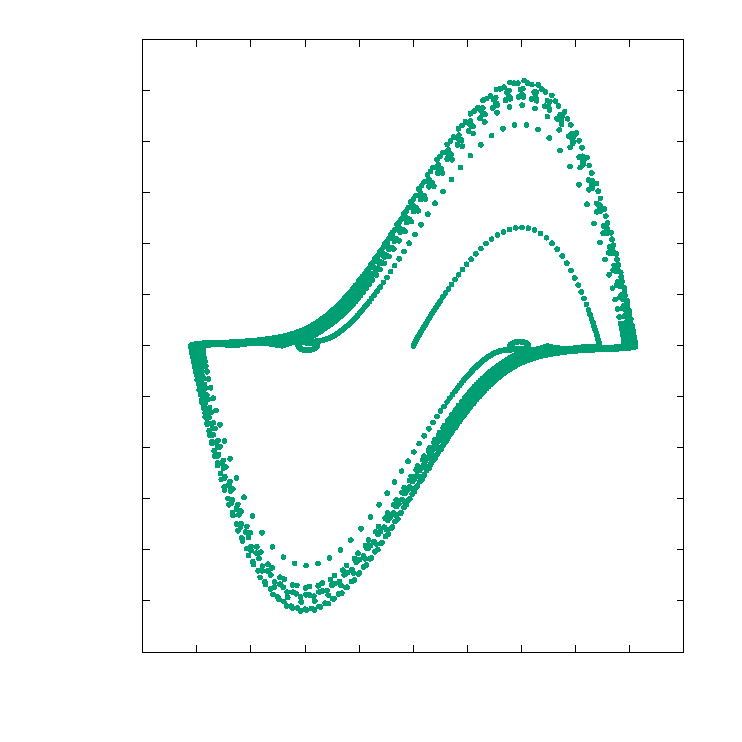
\includegraphics[width={340.10bp},height={340.10bp}]{VDPF8_01_Phase}}%
    \gplfronttext
  \end{picture}%
\endgroup

\end{figure}
\subsubsection{Caos e sensibilità alle condizioni iniziali}
Si è studiata una peculiarità dell'oscillatore di Van der Pol forzato: il cambiamento di regime associato ai diversi valori di $\mu$, visibile anche nelle Fig. \ref{VDPF6} e \ref{VDPF8}. \\
Per osservare qualitativamente la caoticità dei sistemi sono stati graficati gli andamenti $x(t)$ per due condizioni iniziali $x_0$ e $x_0 + dx$ e sono stati osservati i comportamenti dei diversi regimi.
Sono inoltre stati calcolati anche gli esponenti di Lyapunov per ottenere delle stime numeriche della caoticità dei regimi (si veda la Sez. 1.4.1).
\begin{figure}[H]
	\centering
	% GNUPLOT: LaTeX picture with Postscript
\begingroup
  % Encoding inside the plot.  In the header of your document, this encoding
  % should to defined, e.g., by using
  % \usepackage[cp1252,<other encodings>]{inputenc}
  \inputencoding{cp1252}%
  \makeatletter
  \providecommand\color[2][]{%
    \GenericError{(gnuplot) \space\space\space\@spaces}{%
      Package color not loaded in conjunction with
      terminal option `colourtext'%
    }{See the gnuplot documentation for explanation.%
    }{Either use 'blacktext' in gnuplot or load the package
      color.sty in LaTeX.}%
    \renewcommand\color[2][]{}%
  }%
  \providecommand\includegraphics[2][]{%
    \GenericError{(gnuplot) \space\space\space\@spaces}{%
      Package graphicx or graphics not loaded%
    }{See the gnuplot documentation for explanation.%
    }{The gnuplot epslatex terminal needs graphicx.sty or graphics.sty.}%
    \renewcommand\includegraphics[2][]{}%
  }%
  \providecommand\rotatebox[2]{#2}%
  \@ifundefined{ifGPcolor}{%
    \newif\ifGPcolor
    \GPcolortrue
  }{}%
  \@ifundefined{ifGPblacktext}{%
    \newif\ifGPblacktext
    \GPblacktextfalse
  }{}%
  % define a \g@addto@macro without @ in the name:
  \let\gplgaddtomacro\g@addto@macro
  % define empty templates for all commands taking text:
  \gdef\gplbacktext{}%
  \gdef\gplfronttext{}%
  \makeatother
  \ifGPblacktext
    % no textcolor at all
    \def\colorrgb#1{}%
    \def\colorgray#1{}%
  \else
    % gray or color?
    \ifGPcolor
      \def\colorrgb#1{\color[rgb]{#1}}%
      \def\colorgray#1{\color[gray]{#1}}%
      \expandafter\def\csname LTw\endcsname{\color{white}}%
      \expandafter\def\csname LTb\endcsname{\color{black}}%
      \expandafter\def\csname LTa\endcsname{\color{black}}%
      \expandafter\def\csname LT0\endcsname{\color[rgb]{1,0,0}}%
      \expandafter\def\csname LT1\endcsname{\color[rgb]{0,1,0}}%
      \expandafter\def\csname LT2\endcsname{\color[rgb]{0,0,1}}%
      \expandafter\def\csname LT3\endcsname{\color[rgb]{1,0,1}}%
      \expandafter\def\csname LT4\endcsname{\color[rgb]{0,1,1}}%
      \expandafter\def\csname LT5\endcsname{\color[rgb]{1,1,0}}%
      \expandafter\def\csname LT6\endcsname{\color[rgb]{0,0,0}}%
      \expandafter\def\csname LT7\endcsname{\color[rgb]{1,0.3,0}}%
      \expandafter\def\csname LT8\endcsname{\color[rgb]{0.5,0.5,0.5}}%
    \else
      % gray
      \def\colorrgb#1{\color{black}}%
      \def\colorgray#1{\color[gray]{#1}}%
      \expandafter\def\csname LTw\endcsname{\color{white}}%
      \expandafter\def\csname LTb\endcsname{\color{black}}%
      \expandafter\def\csname LTa\endcsname{\color{black}}%
      \expandafter\def\csname LT0\endcsname{\color{black}}%
      \expandafter\def\csname LT1\endcsname{\color{black}}%
      \expandafter\def\csname LT2\endcsname{\color{black}}%
      \expandafter\def\csname LT3\endcsname{\color{black}}%
      \expandafter\def\csname LT4\endcsname{\color{black}}%
      \expandafter\def\csname LT5\endcsname{\color{black}}%
      \expandafter\def\csname LT6\endcsname{\color{black}}%
      \expandafter\def\csname LT7\endcsname{\color{black}}%
      \expandafter\def\csname LT8\endcsname{\color{black}}%
    \fi
  \fi
    \setlength{\unitlength}{0.0500bp}%
    \ifx\gptboxheight\undefined%
      \newlength{\gptboxheight}%
      \newlength{\gptboxwidth}%
      \newsavebox{\gptboxtext}%
    \fi%
    \setlength{\fboxrule}{0.5pt}%
    \setlength{\fboxsep}{1pt}%
    \definecolor{tbcol}{rgb}{1,1,1}%
\begin{picture}(10204.00,5668.00)%
    \gplgaddtomacro\gplbacktext{%
      \csname LTb\endcsname%%
      \put(682,1178){\makebox(0,0)[r]{\strut{}$-2$}}%
      \put(682,2127){\makebox(0,0)[r]{\strut{}$-1$}}%
      \put(682,3076){\makebox(0,0)[r]{\strut{}$0$}}%
      \put(682,4024){\makebox(0,0)[r]{\strut{}$1$}}%
      \put(682,4973){\makebox(0,0)[r]{\strut{}$2$}}%
      \put(814,484){\makebox(0,0){\strut{}$0$}}%
      \put(1713,484){\makebox(0,0){\strut{}$5$}}%
      \put(2613,484){\makebox(0,0){\strut{}$10$}}%
      \put(3512,484){\makebox(0,0){\strut{}$15$}}%
      \put(4411,484){\makebox(0,0){\strut{}$20$}}%
      \put(5311,484){\makebox(0,0){\strut{}$25$}}%
      \put(6210,484){\makebox(0,0){\strut{}$30$}}%
      \put(7109,484){\makebox(0,0){\strut{}$35$}}%
      \put(8008,484){\makebox(0,0){\strut{}$40$}}%
      \put(8908,484){\makebox(0,0){\strut{}$45$}}%
      \put(9807,484){\makebox(0,0){\strut{}$50$}}%
    }%
    \gplgaddtomacro\gplfronttext{%
      \csname LTb\endcsname%%
      \put(209,3075){\rotatebox{-270}{\makebox(0,0){\strut{}x(t)}}}%
      \put(5310,154){\makebox(0,0){\strut{}t}}%
      \csname LTb\endcsname%%
      \put(8820,5219){\makebox(0,0)[r]{\strut{}$x_0 = 2$}}%
      \csname LTb\endcsname%%
      \put(8820,4889){\makebox(0,0)[r]{\strut{}$x_0 = 2.1$}}%
    }%
    \gplbacktext
    \put(0,0){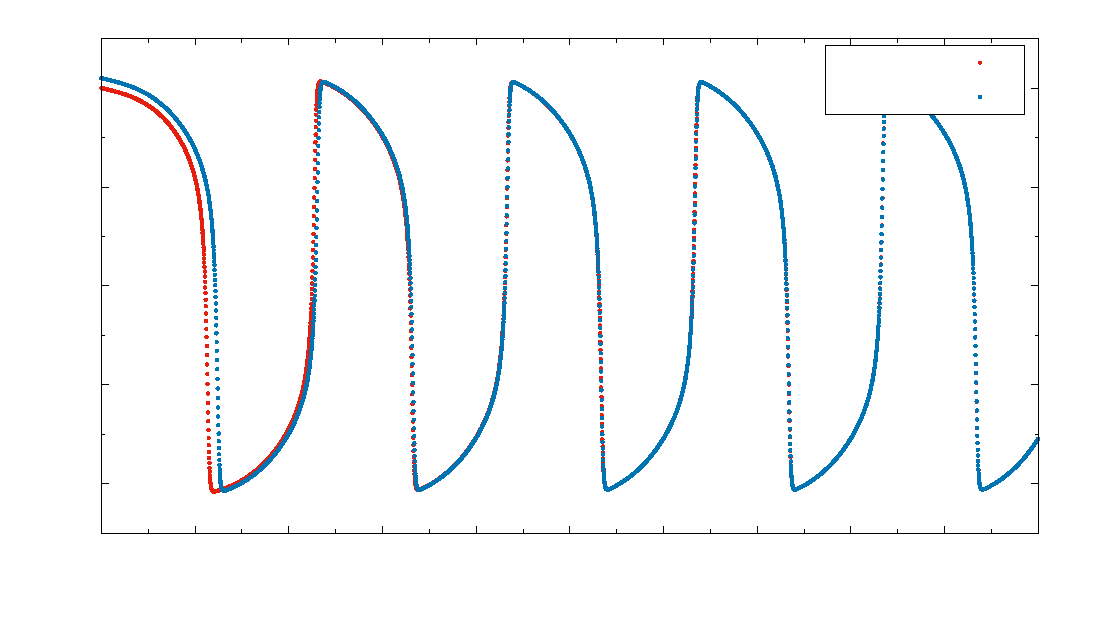
\includegraphics[width={510.20bp},height={283.40bp}]{Caotico1}}%
    \gplfronttext
  \end{picture}%
\endgroup

	\caption{Oscillatore di Van der Pol forzato per $\mu = 6$ e due condizioni iniziali $x_0 = 2$, $x_0 + dx = 2.1$}
	\label{VDPF6_CondIniz}
\end{figure}
\begin{figure}[H]
	\centering
	% GNUPLOT: LaTeX picture with Postscript
\begingroup
  % Encoding inside the plot.  In the header of your document, this encoding
  % should to defined, e.g., by using
  % \usepackage[cp1252,<other encodings>]{inputenc}
  \inputencoding{cp1252}%
  \makeatletter
  \providecommand\color[2][]{%
    \GenericError{(gnuplot) \space\space\space\@spaces}{%
      Package color not loaded in conjunction with
      terminal option `colourtext'%
    }{See the gnuplot documentation for explanation.%
    }{Either use 'blacktext' in gnuplot or load the package
      color.sty in LaTeX.}%
    \renewcommand\color[2][]{}%
  }%
  \providecommand\includegraphics[2][]{%
    \GenericError{(gnuplot) \space\space\space\@spaces}{%
      Package graphicx or graphics not loaded%
    }{See the gnuplot documentation for explanation.%
    }{The gnuplot epslatex terminal needs graphicx.sty or graphics.sty.}%
    \renewcommand\includegraphics[2][]{}%
  }%
  \providecommand\rotatebox[2]{#2}%
  \@ifundefined{ifGPcolor}{%
    \newif\ifGPcolor
    \GPcolortrue
  }{}%
  \@ifundefined{ifGPblacktext}{%
    \newif\ifGPblacktext
    \GPblacktextfalse
  }{}%
  % define a \g@addto@macro without @ in the name:
  \let\gplgaddtomacro\g@addto@macro
  % define empty templates for all commands taking text:
  \gdef\gplbacktext{}%
  \gdef\gplfronttext{}%
  \makeatother
  \ifGPblacktext
    % no textcolor at all
    \def\colorrgb#1{}%
    \def\colorgray#1{}%
  \else
    % gray or color?
    \ifGPcolor
      \def\colorrgb#1{\color[rgb]{#1}}%
      \def\colorgray#1{\color[gray]{#1}}%
      \expandafter\def\csname LTw\endcsname{\color{white}}%
      \expandafter\def\csname LTb\endcsname{\color{black}}%
      \expandafter\def\csname LTa\endcsname{\color{black}}%
      \expandafter\def\csname LT0\endcsname{\color[rgb]{1,0,0}}%
      \expandafter\def\csname LT1\endcsname{\color[rgb]{0,1,0}}%
      \expandafter\def\csname LT2\endcsname{\color[rgb]{0,0,1}}%
      \expandafter\def\csname LT3\endcsname{\color[rgb]{1,0,1}}%
      \expandafter\def\csname LT4\endcsname{\color[rgb]{0,1,1}}%
      \expandafter\def\csname LT5\endcsname{\color[rgb]{1,1,0}}%
      \expandafter\def\csname LT6\endcsname{\color[rgb]{0,0,0}}%
      \expandafter\def\csname LT7\endcsname{\color[rgb]{1,0.3,0}}%
      \expandafter\def\csname LT8\endcsname{\color[rgb]{0.5,0.5,0.5}}%
    \else
      % gray
      \def\colorrgb#1{\color{black}}%
      \def\colorgray#1{\color[gray]{#1}}%
      \expandafter\def\csname LTw\endcsname{\color{white}}%
      \expandafter\def\csname LTb\endcsname{\color{black}}%
      \expandafter\def\csname LTa\endcsname{\color{black}}%
      \expandafter\def\csname LT0\endcsname{\color{black}}%
      \expandafter\def\csname LT1\endcsname{\color{black}}%
      \expandafter\def\csname LT2\endcsname{\color{black}}%
      \expandafter\def\csname LT3\endcsname{\color{black}}%
      \expandafter\def\csname LT4\endcsname{\color{black}}%
      \expandafter\def\csname LT5\endcsname{\color{black}}%
      \expandafter\def\csname LT6\endcsname{\color{black}}%
      \expandafter\def\csname LT7\endcsname{\color{black}}%
      \expandafter\def\csname LT8\endcsname{\color{black}}%
    \fi
  \fi
    \setlength{\unitlength}{0.0500bp}%
    \ifx\gptboxheight\undefined%
      \newlength{\gptboxheight}%
      \newlength{\gptboxwidth}%
      \newsavebox{\gptboxtext}%
    \fi%
    \setlength{\fboxrule}{0.5pt}%
    \setlength{\fboxsep}{1pt}%
    \definecolor{tbcol}{rgb}{1,1,1}%
\begin{picture}(10204.00,5668.00)%
    \gplgaddtomacro\gplbacktext{%
      \csname LTb\endcsname%%
      \put(682,1178){\makebox(0,0)[r]{\strut{}$-2$}}%
      \put(682,2127){\makebox(0,0)[r]{\strut{}$-1$}}%
      \put(682,3076){\makebox(0,0)[r]{\strut{}$0$}}%
      \put(682,4024){\makebox(0,0)[r]{\strut{}$1$}}%
      \put(682,4973){\makebox(0,0)[r]{\strut{}$2$}}%
      \put(814,484){\makebox(0,0){\strut{}$0$}}%
      \put(1264,484){\makebox(0,0){\strut{}$5$}}%
      \put(1713,484){\makebox(0,0){\strut{}$10$}}%
      \put(2163,484){\makebox(0,0){\strut{}$15$}}%
      \put(2613,484){\makebox(0,0){\strut{}$20$}}%
      \put(3062,484){\makebox(0,0){\strut{}$25$}}%
      \put(3512,484){\makebox(0,0){\strut{}$30$}}%
      \put(3962,484){\makebox(0,0){\strut{}$35$}}%
      \put(4411,484){\makebox(0,0){\strut{}$40$}}%
      \put(4861,484){\makebox(0,0){\strut{}$45$}}%
      \put(5310,484){\makebox(0,0){\strut{}$50$}}%
      \put(5760,484){\makebox(0,0){\strut{}$55$}}%
      \put(6210,484){\makebox(0,0){\strut{}$60$}}%
      \put(6659,484){\makebox(0,0){\strut{}$65$}}%
      \put(7109,484){\makebox(0,0){\strut{}$70$}}%
      \put(7559,484){\makebox(0,0){\strut{}$75$}}%
      \put(8008,484){\makebox(0,0){\strut{}$80$}}%
      \put(8458,484){\makebox(0,0){\strut{}$85$}}%
      \put(8908,484){\makebox(0,0){\strut{}$90$}}%
      \put(9357,484){\makebox(0,0){\strut{}$95$}}%
      \put(9807,484){\makebox(0,0){\strut{}$100$}}%
    }%
    \gplgaddtomacro\gplfronttext{%
      \csname LTb\endcsname%%
      \put(209,3075){\rotatebox{-270}{\makebox(0,0){\strut{}x(t)}}}%
      \put(5310,154){\makebox(0,0){\strut{}t}}%
      \csname LTb\endcsname%%
      \put(8820,5219){\makebox(0,0)[r]{\strut{}$x_0 = 2$}}%
      \csname LTb\endcsname%%
      \put(8820,4889){\makebox(0,0)[r]{\strut{}$x_0 = 2.1$}}%
    }%
    \gplbacktext
    \put(0,0){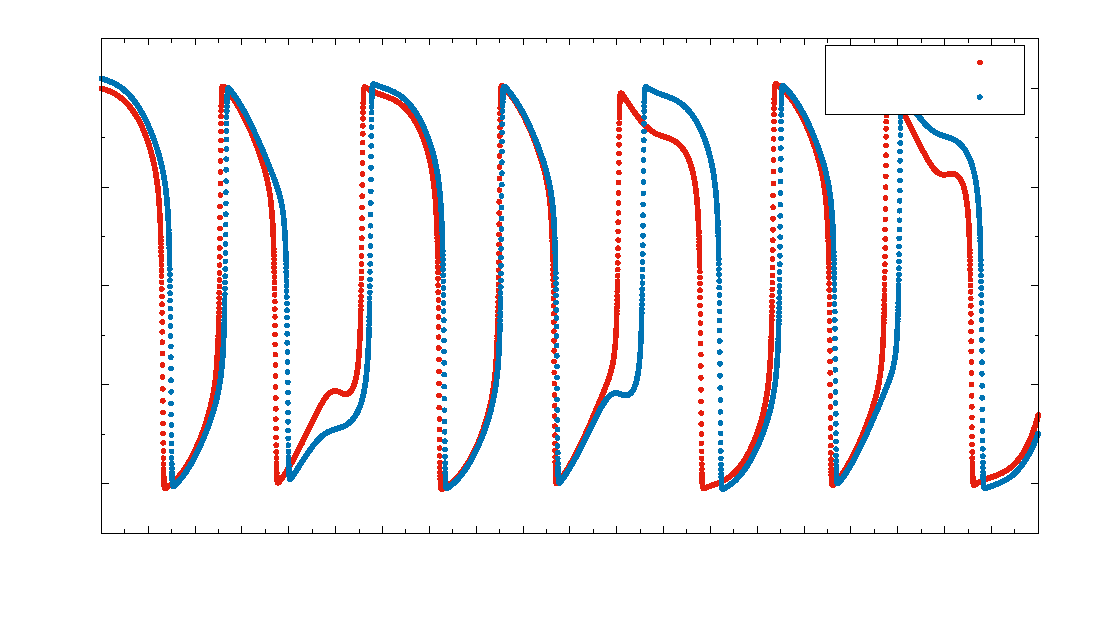
\includegraphics[width={510.20bp},height={283.40bp}]{Caotico3}}%
    \gplfronttext
  \end{picture}%
\endgroup

	\caption{Oscillatore di Van der Pol forzato per $\mu = 8$ e due condizioni iniziali $x_0 = 2$, $x_0 + dx = 2.1$}
	\label{VDPF8_CondIniz}
\end{figure}
Risulta ben evidente la sensibilità alle condizioni iniziali del regime in Fig. \ref{VDPF8_CondIniz}: le due traiettorie si discostano rapidamente, al contrario di quanto accade in Fig. \ref{VDPF6_CondIniz}, in cui invece le traiettorie vanno a sovrapporsi.
\subsection{Equazioni rigide e ordine di accuratezza}
Un'equazione differenziale si dice rigida (o stiff) quando certi di metodi di soluzione sono numericamente instabili a meno che il passo d'integrazione sia preso estremamente piccolo. L'idea generale della definizione di rigidità è che l'equazione includa dei termini che possono portare a rapide variazioni delle soluzioni. \\ \\
In questo caso è utile anche introdurre il concetto di ordine di accuratezza di una soluzione numerica. \\
L'ordine di accuratezza quantifica il tasso di convergenza della soluzione approssimata dell'equazione differenziale alla sua soluzione esatta. \\
Stiamo parlando di funzioni, quindi ci posizioniamo in uno spazio normato di funzioni $(V,||\cdot||)$, dove la norma deve essere scelta opportunamente, e si considera che l'equazione abbia una soluzione esatta $v$ e una soluzione numerica approssimata $v_h$, dove $h$ è il parametro che caratterizza l'approssimazione, quindi il time step. \\
A questo punto si dice che la soluzione $v_h$ ha un'accuratezza di ordine n se l'errore
\begin{equation}
	E(h) = ||v-v_h|| \leq Ch
\end{equation}
dove $C$ è una costante indipendente da $h$ che dipende solo dalla soluzione $v$. \\
Possiamo esprimere questo concetto con la notazione degli O-grandi:
\begin{equation}
	||v-v_h|| = O(h^n)
\end{equation}
Questa definizione dipende fortemente dalla norma usata nello spazio $V$, e quindi la scelta di questa norma è essenziale per calcolare correttamente il tasso di convergenza delle soluzioni approssimate. \\ \\
L'equazione di Van Der Pol è un'equazione che cade nella definizione di equazione rigida, quindi per risolverla correttamente è essenziale scegliere dei time-step abbastanza piccoli. La rigidità (stiffness) di quest'equazione è contenuta nella costante $\mu$, e questo può essere visualizzato confrontando le soluzioni ottenute variando i time step. Per fare ciò confrontiamo prima gli andamenti temporali delle $x$ e delle $p$, e in seguito le traiettorie nello spazio delle fasi, per valori di $\mu$ dell'ordine dell'unità, e in seguito alziamo il valore di $\mu$ e rifacciamo questo confronto, per verificare come cambino i risultati.
\subsubsection{Confronto sulla rigidità per $\mu = 1$}
Come detto, il parametro $\mu$ determina la rigidità dell'equazione di Van Der Pol, quindi per $\mu = 1$ l'equazione sarà poco rigida, e ne risulta che si potranno ottenere soluzioni accurate con tipe step non eccessivamente brevi. \\ \\
Confrontando i risultati con le soluzioni "esatte" trovate in rete si è notato che con questa rigidità, si può ottenere una soluzione quasi identica alla soluzione "esatta" utilizzando un time step di $h = 10^{-4}$, quindi si è preso questo valore come riferimento e si sono considerate le traiettorie ottenute mediante esso come esatte. \\ \\
Confrontiamo prima l'andamento temporale della $x(t)$. Questo confronto viene fatto per $\Delta t = 0.1$, $\Delta t = 0.01$ e $\Delta t = 0.001$. Si è provato anche a usare un timestep $h=1$, ma la soluzione è risultata altamente instabile, a indicare che questo valore sia troppo piccolo per risolvere quest'equazione. 
\begin{figure}[H]
	\centering
	\scalebox{0.9}{% GNUPLOT: LaTeX picture with Postscript
\begingroup
  % Encoding inside the plot.  In the header of your document, this encoding
  % should to defined, e.g., by using
  % \usepackage[cp1252,<other encodings>]{inputenc}
  \inputencoding{cp1252}%
  \makeatletter
  \providecommand\color[2][]{%
    \GenericError{(gnuplot) \space\space\space\@spaces}{%
      Package color not loaded in conjunction with
      terminal option `colourtext'%
    }{See the gnuplot documentation for explanation.%
    }{Either use 'blacktext' in gnuplot or load the package
      color.sty in LaTeX.}%
    \renewcommand\color[2][]{}%
  }%
  \providecommand\includegraphics[2][]{%
    \GenericError{(gnuplot) \space\space\space\@spaces}{%
      Package graphicx or graphics not loaded%
    }{See the gnuplot documentation for explanation.%
    }{The gnuplot epslatex terminal needs graphicx.sty or graphics.sty.}%
    \renewcommand\includegraphics[2][]{}%
  }%
  \providecommand\rotatebox[2]{#2}%
  \@ifundefined{ifGPcolor}{%
    \newif\ifGPcolor
    \GPcolortrue
  }{}%
  \@ifundefined{ifGPblacktext}{%
    \newif\ifGPblacktext
    \GPblacktextfalse
  }{}%
  % define a \g@addto@macro without @ in the name:
  \let\gplgaddtomacro\g@addto@macro
  % define empty templates for all commands taking text:
  \gdef\gplbacktext{}%
  \gdef\gplfronttext{}%
  \makeatother
  \ifGPblacktext
    % no textcolor at all
    \def\colorrgb#1{}%
    \def\colorgray#1{}%
  \else
    % gray or color?
    \ifGPcolor
      \def\colorrgb#1{\color[rgb]{#1}}%
      \def\colorgray#1{\color[gray]{#1}}%
      \expandafter\def\csname LTw\endcsname{\color{white}}%
      \expandafter\def\csname LTb\endcsname{\color{black}}%
      \expandafter\def\csname LTa\endcsname{\color{black}}%
      \expandafter\def\csname LT0\endcsname{\color[rgb]{1,0,0}}%
      \expandafter\def\csname LT1\endcsname{\color[rgb]{0,1,0}}%
      \expandafter\def\csname LT2\endcsname{\color[rgb]{0,0,1}}%
      \expandafter\def\csname LT3\endcsname{\color[rgb]{1,0,1}}%
      \expandafter\def\csname LT4\endcsname{\color[rgb]{0,1,1}}%
      \expandafter\def\csname LT5\endcsname{\color[rgb]{1,1,0}}%
      \expandafter\def\csname LT6\endcsname{\color[rgb]{0,0,0}}%
      \expandafter\def\csname LT7\endcsname{\color[rgb]{1,0.3,0}}%
      \expandafter\def\csname LT8\endcsname{\color[rgb]{0.5,0.5,0.5}}%
    \else
      % gray
      \def\colorrgb#1{\color{black}}%
      \def\colorgray#1{\color[gray]{#1}}%
      \expandafter\def\csname LTw\endcsname{\color{white}}%
      \expandafter\def\csname LTb\endcsname{\color{black}}%
      \expandafter\def\csname LTa\endcsname{\color{black}}%
      \expandafter\def\csname LT0\endcsname{\color{black}}%
      \expandafter\def\csname LT1\endcsname{\color{black}}%
      \expandafter\def\csname LT2\endcsname{\color{black}}%
      \expandafter\def\csname LT3\endcsname{\color{black}}%
      \expandafter\def\csname LT4\endcsname{\color{black}}%
      \expandafter\def\csname LT5\endcsname{\color{black}}%
      \expandafter\def\csname LT6\endcsname{\color{black}}%
      \expandafter\def\csname LT7\endcsname{\color{black}}%
      \expandafter\def\csname LT8\endcsname{\color{black}}%
    \fi
  \fi
    \setlength{\unitlength}{0.0500bp}%
    \ifx\gptboxheight\undefined%
      \newlength{\gptboxheight}%
      \newlength{\gptboxwidth}%
      \newsavebox{\gptboxtext}%
    \fi%
    \setlength{\fboxrule}{0.5pt}%
    \setlength{\fboxsep}{1pt}%
    \definecolor{tbcol}{rgb}{1,1,1}%
\begin{picture}(10204.00,6802.00)%
    \gplgaddtomacro\gplbacktext{%
      \csname LTb\endcsname%%
      \put(946,704){\makebox(0,0)[r]{\strut{}$-2.5$}}%
      \put(946,1292){\makebox(0,0)[r]{\strut{}$-2$}}%
      \put(946,1879){\makebox(0,0)[r]{\strut{}$-1.5$}}%
      \put(946,2467){\makebox(0,0)[r]{\strut{}$-1$}}%
      \put(946,3055){\makebox(0,0)[r]{\strut{}$-0.5$}}%
      \put(946,3643){\makebox(0,0)[r]{\strut{}$0$}}%
      \put(946,4230){\makebox(0,0)[r]{\strut{}$0.5$}}%
      \put(946,4818){\makebox(0,0)[r]{\strut{}$1$}}%
      \put(946,5406){\makebox(0,0)[r]{\strut{}$1.5$}}%
      \put(946,5993){\makebox(0,0)[r]{\strut{}$2$}}%
      \put(946,6581){\makebox(0,0)[r]{\strut{}$2.5$}}%
      \put(1078,484){\makebox(0,0){\strut{}$0$}}%
      \put(2169,484){\makebox(0,0){\strut{}$2$}}%
      \put(3260,484){\makebox(0,0){\strut{}$4$}}%
      \put(4351,484){\makebox(0,0){\strut{}$6$}}%
      \put(5443,484){\makebox(0,0){\strut{}$8$}}%
      \put(6534,484){\makebox(0,0){\strut{}$10$}}%
      \put(7625,484){\makebox(0,0){\strut{}$12$}}%
      \put(8716,484){\makebox(0,0){\strut{}$14$}}%
      \put(9807,484){\makebox(0,0){\strut{}$16$}}%
    }%
    \gplgaddtomacro\gplfronttext{%
      \csname LTb\endcsname%%
      \put(209,3642){\rotatebox{-270}{\makebox(0,0){\strut{}x(t)}}}%
      \put(5442,154){\makebox(0,0){\strut{}t}}%
      \csname LTb\endcsname%%
      \put(2530,6353){\makebox(0,0)[r]{\strut{}$h = 0.0001$}}%
      \csname LTb\endcsname%%
      \put(2530,6023){\makebox(0,0)[r]{\strut{}$h = 0.001$}}%
      \csname LTb\endcsname%%
      \put(2530,5693){\makebox(0,0)[r]{\strut{}$h = 0.01$}}%
      \csname LTb\endcsname%%
      \put(2530,5363){\makebox(0,0)[r]{\strut{}$h = 0.1$}}%
    }%
    \gplgaddtomacro\gplbacktext{%
      \csname LTb\endcsname%%
      \put(946,704){\makebox(0,0)[r]{\strut{}$-2.5$}}%
      \put(946,1292){\makebox(0,0)[r]{\strut{}$-2$}}%
      \put(946,1879){\makebox(0,0)[r]{\strut{}$-1.5$}}%
      \put(946,2467){\makebox(0,0)[r]{\strut{}$-1$}}%
      \put(946,3055){\makebox(0,0)[r]{\strut{}$-0.5$}}%
      \put(946,3643){\makebox(0,0)[r]{\strut{}$0$}}%
      \put(946,4230){\makebox(0,0)[r]{\strut{}$0.5$}}%
      \put(946,4818){\makebox(0,0)[r]{\strut{}$1$}}%
      \put(946,5406){\makebox(0,0)[r]{\strut{}$1.5$}}%
      \put(946,5993){\makebox(0,0)[r]{\strut{}$2$}}%
      \put(946,6581){\makebox(0,0)[r]{\strut{}$2.5$}}%
      \put(1078,484){\makebox(0,0){\strut{}$0$}}%
      \put(2169,484){\makebox(0,0){\strut{}$2$}}%
      \put(3260,484){\makebox(0,0){\strut{}$4$}}%
      \put(4351,484){\makebox(0,0){\strut{}$6$}}%
      \put(5443,484){\makebox(0,0){\strut{}$8$}}%
      \put(6534,484){\makebox(0,0){\strut{}$10$}}%
      \put(7625,484){\makebox(0,0){\strut{}$12$}}%
      \put(8716,484){\makebox(0,0){\strut{}$14$}}%
      \put(9807,484){\makebox(0,0){\strut{}$16$}}%
    }%
    \gplgaddtomacro\gplfronttext{%
      \csname LTb\endcsname%%
      \put(209,3642){\rotatebox{-270}{\makebox(0,0){\strut{}x(t)}}}%
      \put(5442,154){\makebox(0,0){\strut{}t}}%
      \csname LTb\endcsname%%
      \put(2530,6353){\makebox(0,0)[r]{\strut{}$h = 0.0001$}}%
      \csname LTb\endcsname%%
      \put(2530,6023){\makebox(0,0)[r]{\strut{}$h = 0.001$}}%
      \csname LTb\endcsname%%
      \put(2530,5693){\makebox(0,0)[r]{\strut{}$h = 0.01$}}%
      \csname LTb\endcsname%%
      \put(2530,5363){\makebox(0,0)[r]{\strut{}$h = 0.1$}}%
    }%
    \gplbacktext
    \put(0,0){\includegraphics[width={510.20bp},height={340.10bp}]{ConfrXGGG}}%
    \gplfronttext
  \end{picture}%
\endgroup
}
\end{figure}
\begin{figure}[H]
	\centering
	% GNUPLOT: LaTeX picture with Postscript
\begingroup
  % Encoding inside the plot.  In the header of your document, this encoding
  % should to defined, e.g., by using
  % \usepackage[cp1252,<other encodings>]{inputenc}
  \inputencoding{cp1252}%
  \makeatletter
  \providecommand\color[2][]{%
    \GenericError{(gnuplot) \space\space\space\@spaces}{%
      Package color not loaded in conjunction with
      terminal option `colourtext'%
    }{See the gnuplot documentation for explanation.%
    }{Either use 'blacktext' in gnuplot or load the package
      color.sty in LaTeX.}%
    \renewcommand\color[2][]{}%
  }%
  \providecommand\includegraphics[2][]{%
    \GenericError{(gnuplot) \space\space\space\@spaces}{%
      Package graphicx or graphics not loaded%
    }{See the gnuplot documentation for explanation.%
    }{The gnuplot epslatex terminal needs graphicx.sty or graphics.sty.}%
    \renewcommand\includegraphics[2][]{}%
  }%
  \providecommand\rotatebox[2]{#2}%
  \@ifundefined{ifGPcolor}{%
    \newif\ifGPcolor
    \GPcolortrue
  }{}%
  \@ifundefined{ifGPblacktext}{%
    \newif\ifGPblacktext
    \GPblacktextfalse
  }{}%
  % define a \g@addto@macro without @ in the name:
  \let\gplgaddtomacro\g@addto@macro
  % define empty templates for all commands taking text:
  \gdef\gplbacktext{}%
  \gdef\gplfronttext{}%
  \makeatother
  \ifGPblacktext
    % no textcolor at all
    \def\colorrgb#1{}%
    \def\colorgray#1{}%
  \else
    % gray or color?
    \ifGPcolor
      \def\colorrgb#1{\color[rgb]{#1}}%
      \def\colorgray#1{\color[gray]{#1}}%
      \expandafter\def\csname LTw\endcsname{\color{white}}%
      \expandafter\def\csname LTb\endcsname{\color{black}}%
      \expandafter\def\csname LTa\endcsname{\color{black}}%
      \expandafter\def\csname LT0\endcsname{\color[rgb]{1,0,0}}%
      \expandafter\def\csname LT1\endcsname{\color[rgb]{0,1,0}}%
      \expandafter\def\csname LT2\endcsname{\color[rgb]{0,0,1}}%
      \expandafter\def\csname LT3\endcsname{\color[rgb]{1,0,1}}%
      \expandafter\def\csname LT4\endcsname{\color[rgb]{0,1,1}}%
      \expandafter\def\csname LT5\endcsname{\color[rgb]{1,1,0}}%
      \expandafter\def\csname LT6\endcsname{\color[rgb]{0,0,0}}%
      \expandafter\def\csname LT7\endcsname{\color[rgb]{1,0.3,0}}%
      \expandafter\def\csname LT8\endcsname{\color[rgb]{0.5,0.5,0.5}}%
    \else
      % gray
      \def\colorrgb#1{\color{black}}%
      \def\colorgray#1{\color[gray]{#1}}%
      \expandafter\def\csname LTw\endcsname{\color{white}}%
      \expandafter\def\csname LTb\endcsname{\color{black}}%
      \expandafter\def\csname LTa\endcsname{\color{black}}%
      \expandafter\def\csname LT0\endcsname{\color{black}}%
      \expandafter\def\csname LT1\endcsname{\color{black}}%
      \expandafter\def\csname LT2\endcsname{\color{black}}%
      \expandafter\def\csname LT3\endcsname{\color{black}}%
      \expandafter\def\csname LT4\endcsname{\color{black}}%
      \expandafter\def\csname LT5\endcsname{\color{black}}%
      \expandafter\def\csname LT6\endcsname{\color{black}}%
      \expandafter\def\csname LT7\endcsname{\color{black}}%
      \expandafter\def\csname LT8\endcsname{\color{black}}%
    \fi
  \fi
    \setlength{\unitlength}{0.0500bp}%
    \ifx\gptboxheight\undefined%
      \newlength{\gptboxheight}%
      \newlength{\gptboxwidth}%
      \newsavebox{\gptboxtext}%
    \fi%
    \setlength{\fboxrule}{0.5pt}%
    \setlength{\fboxsep}{1pt}%
    \definecolor{tbcol}{rgb}{1,1,1}%
\begin{picture}(10204.00,5668.00)%
    \gplgaddtomacro\gplbacktext{%
      \csname LTb\endcsname%%
      \put(946,704){\makebox(0,0)[r]{\strut{}$-1.4$}}%
      \put(946,1178){\makebox(0,0)[r]{\strut{}$-1.3$}}%
      \put(946,1653){\makebox(0,0)[r]{\strut{}$-1.2$}}%
      \put(946,2127){\makebox(0,0)[r]{\strut{}$-1.1$}}%
      \put(946,2601){\makebox(0,0)[r]{\strut{}$-1$}}%
      \put(946,3076){\makebox(0,0)[r]{\strut{}$-0.9$}}%
      \put(946,3550){\makebox(0,0)[r]{\strut{}$-0.8$}}%
      \put(946,4024){\makebox(0,0)[r]{\strut{}$-0.7$}}%
      \put(946,4498){\makebox(0,0)[r]{\strut{}$-0.6$}}%
      \put(946,4973){\makebox(0,0)[r]{\strut{}$-0.5$}}%
      \put(946,5447){\makebox(0,0)[r]{\strut{}$-0.4$}}%
      \put(1078,484){\makebox(0,0){\strut{}$8.5$}}%
      \put(3260,484){\makebox(0,0){\strut{}$9$}}%
      \put(5443,484){\makebox(0,0){\strut{}$9.5$}}%
      \put(7625,484){\makebox(0,0){\strut{}$10$}}%
      \put(9807,484){\makebox(0,0){\strut{}$10.5$}}%
    }%
    \gplgaddtomacro\gplfronttext{%
      \csname LTb\endcsname%%
      \put(209,3075){\rotatebox{-270}{\makebox(0,0){\strut{}x(t)}}}%
      \put(5442,154){\makebox(0,0){\strut{}t}}%
      \csname LTb\endcsname%%
      \put(2530,5219){\makebox(0,0)[r]{\strut{}$h = 0.0001$}}%
      \csname LTb\endcsname%%
      \put(2530,4889){\makebox(0,0)[r]{\strut{}$h = 0.001$}}%
      \csname LTb\endcsname%%
      \put(2530,4559){\makebox(0,0)[r]{\strut{}$h = 0.01$}}%
      \csname LTb\endcsname%%
      \put(2530,4229){\makebox(0,0)[r]{\strut{}$h = 0.1$}}%
    }%
    \gplbacktext
    \put(0,0){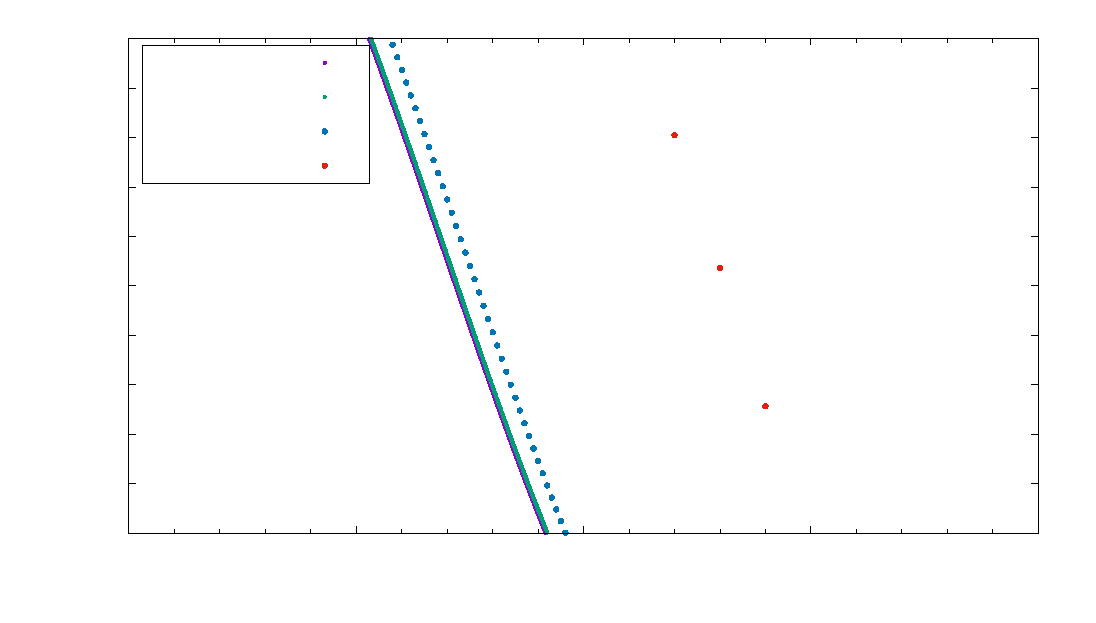
\includegraphics[width={510.20bp},height={283.40bp}]{ConfrXZ}}%
    \gplfronttext
  \end{picture}%
\endgroup

\end{figure}
Come si può vedere nel grafico soprastante, per $\Delta t = 0.001$ si ottiene una curva quasi identica a quella considerata esatta, per $\Delta t = 0.01$ si ottiene una curva molto molto simile mentre per $\Delta t = 0.1$ si ottiene una curva decisamente diversa, ad indicare che questo time step è troppo lungo per risolvere l'equazione con questo grado di rigidità in maniera precisa e soddisfacente. \\
Nel grafico soprastante si può vedere uno zoom del grafico precedente, che permette di osservare che le curve verdi e viola siano effettivamente quasi identiche, infatti sono quasi completamente sovrapposte. \\
Ora confrontiamo l'andamento temporale di $p(t)$: 
\begin{figure}[H]
	\centering
	% GNUPLOT: LaTeX picture with Postscript
\begingroup
  % Encoding inside the plot.  In the header of your document, this encoding
  % should to defined, e.g., by using
  % \usepackage[cp1252,<other encodings>]{inputenc}
  \inputencoding{cp1252}%
  \makeatletter
  \providecommand\color[2][]{%
    \GenericError{(gnuplot) \space\space\space\@spaces}{%
      Package color not loaded in conjunction with
      terminal option `colourtext'%
    }{See the gnuplot documentation for explanation.%
    }{Either use 'blacktext' in gnuplot or load the package
      color.sty in LaTeX.}%
    \renewcommand\color[2][]{}%
  }%
  \providecommand\includegraphics[2][]{%
    \GenericError{(gnuplot) \space\space\space\@spaces}{%
      Package graphicx or graphics not loaded%
    }{See the gnuplot documentation for explanation.%
    }{The gnuplot epslatex terminal needs graphicx.sty or graphics.sty.}%
    \renewcommand\includegraphics[2][]{}%
  }%
  \providecommand\rotatebox[2]{#2}%
  \@ifundefined{ifGPcolor}{%
    \newif\ifGPcolor
    \GPcolortrue
  }{}%
  \@ifundefined{ifGPblacktext}{%
    \newif\ifGPblacktext
    \GPblacktextfalse
  }{}%
  % define a \g@addto@macro without @ in the name:
  \let\gplgaddtomacro\g@addto@macro
  % define empty templates for all commands taking text:
  \gdef\gplbacktext{}%
  \gdef\gplfronttext{}%
  \makeatother
  \ifGPblacktext
    % no textcolor at all
    \def\colorrgb#1{}%
    \def\colorgray#1{}%
  \else
    % gray or color?
    \ifGPcolor
      \def\colorrgb#1{\color[rgb]{#1}}%
      \def\colorgray#1{\color[gray]{#1}}%
      \expandafter\def\csname LTw\endcsname{\color{white}}%
      \expandafter\def\csname LTb\endcsname{\color{black}}%
      \expandafter\def\csname LTa\endcsname{\color{black}}%
      \expandafter\def\csname LT0\endcsname{\color[rgb]{1,0,0}}%
      \expandafter\def\csname LT1\endcsname{\color[rgb]{0,1,0}}%
      \expandafter\def\csname LT2\endcsname{\color[rgb]{0,0,1}}%
      \expandafter\def\csname LT3\endcsname{\color[rgb]{1,0,1}}%
      \expandafter\def\csname LT4\endcsname{\color[rgb]{0,1,1}}%
      \expandafter\def\csname LT5\endcsname{\color[rgb]{1,1,0}}%
      \expandafter\def\csname LT6\endcsname{\color[rgb]{0,0,0}}%
      \expandafter\def\csname LT7\endcsname{\color[rgb]{1,0.3,0}}%
      \expandafter\def\csname LT8\endcsname{\color[rgb]{0.5,0.5,0.5}}%
    \else
      % gray
      \def\colorrgb#1{\color{black}}%
      \def\colorgray#1{\color[gray]{#1}}%
      \expandafter\def\csname LTw\endcsname{\color{white}}%
      \expandafter\def\csname LTb\endcsname{\color{black}}%
      \expandafter\def\csname LTa\endcsname{\color{black}}%
      \expandafter\def\csname LT0\endcsname{\color{black}}%
      \expandafter\def\csname LT1\endcsname{\color{black}}%
      \expandafter\def\csname LT2\endcsname{\color{black}}%
      \expandafter\def\csname LT3\endcsname{\color{black}}%
      \expandafter\def\csname LT4\endcsname{\color{black}}%
      \expandafter\def\csname LT5\endcsname{\color{black}}%
      \expandafter\def\csname LT6\endcsname{\color{black}}%
      \expandafter\def\csname LT7\endcsname{\color{black}}%
      \expandafter\def\csname LT8\endcsname{\color{black}}%
    \fi
  \fi
    \setlength{\unitlength}{0.0500bp}%
    \ifx\gptboxheight\undefined%
      \newlength{\gptboxheight}%
      \newlength{\gptboxwidth}%
      \newsavebox{\gptboxtext}%
    \fi%
    \setlength{\fboxrule}{0.5pt}%
    \setlength{\fboxsep}{1pt}%
    \definecolor{tbcol}{rgb}{1,1,1}%
\begin{picture}(10204.00,5668.00)%
    \gplgaddtomacro\gplbacktext{%
      \csname LTb\endcsname%%
      \put(682,704){\makebox(0,0)[r]{\strut{}$-3$}}%
      \put(682,1495){\makebox(0,0)[r]{\strut{}$-2$}}%
      \put(682,2285){\makebox(0,0)[r]{\strut{}$-1$}}%
      \put(682,3076){\makebox(0,0)[r]{\strut{}$0$}}%
      \put(682,3866){\makebox(0,0)[r]{\strut{}$1$}}%
      \put(682,4657){\makebox(0,0)[r]{\strut{}$2$}}%
      \put(682,5447){\makebox(0,0)[r]{\strut{}$3$}}%
      \put(814,484){\makebox(0,0){\strut{}$0$}}%
      \put(1394,484){\makebox(0,0){\strut{}$1$}}%
      \put(1974,484){\makebox(0,0){\strut{}$2$}}%
      \put(2555,484){\makebox(0,0){\strut{}$3$}}%
      \put(3135,484){\makebox(0,0){\strut{}$4$}}%
      \put(3715,484){\makebox(0,0){\strut{}$5$}}%
      \put(4295,484){\makebox(0,0){\strut{}$6$}}%
      \put(4875,484){\makebox(0,0){\strut{}$7$}}%
      \put(5456,484){\makebox(0,0){\strut{}$8$}}%
      \put(6036,484){\makebox(0,0){\strut{}$9$}}%
      \put(6616,484){\makebox(0,0){\strut{}$10$}}%
      \put(7196,484){\makebox(0,0){\strut{}$11$}}%
      \put(7776,484){\makebox(0,0){\strut{}$12$}}%
      \put(8357,484){\makebox(0,0){\strut{}$13$}}%
      \put(8937,484){\makebox(0,0){\strut{}$14$}}%
      \put(9517,484){\makebox(0,0){\strut{}$15$}}%
    }%
    \gplgaddtomacro\gplfronttext{%
      \csname LTb\endcsname%%
      \put(209,3075){\rotatebox{-270}{\makebox(0,0){\strut{}p(t)}}}%
      \put(5310,154){\makebox(0,0){\strut{}t}}%
      \csname LTb\endcsname%%
      \put(2266,5219){\makebox(0,0)[r]{\strut{}$h = 0.0001$}}%
      \csname LTb\endcsname%%
      \put(2266,4889){\makebox(0,0)[r]{\strut{}$h = 0.001$}}%
      \csname LTb\endcsname%%
      \put(2266,4559){\makebox(0,0)[r]{\strut{}$h = 0.01$}}%
      \csname LTb\endcsname%%
      \put(2266,4229){\makebox(0,0)[r]{\strut{}$h = 0.1$}}%
    }%
    \gplbacktext
    \put(0,0){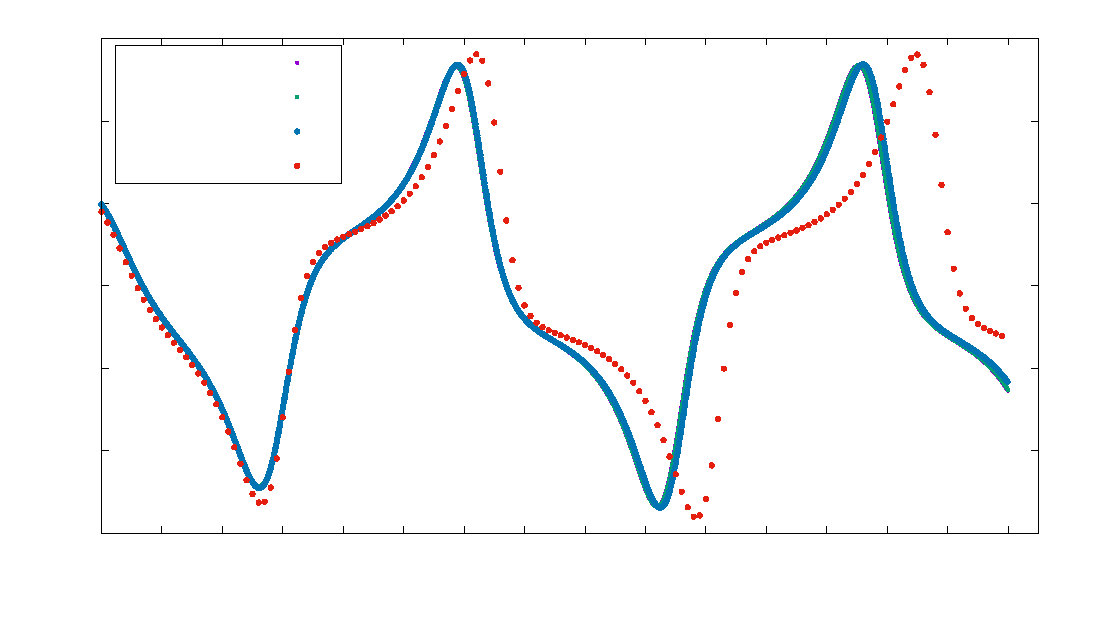
\includegraphics[width={510.20bp},height={283.40bp}]{ConfrP}}%
    \gplfronttext
  \end{picture}%
\endgroup

\end{figure}
e vediamo un comportamento molto simile a quanto visto per $x(t)$. 
\begin{figure}[H]
	\centering
	% GNUPLOT: LaTeX picture with Postscript
\begingroup
  % Encoding inside the plot.  In the header of your document, this encoding
  % should to defined, e.g., by using
  % \usepackage[cp1252,<other encodings>]{inputenc}
  \inputencoding{cp1252}%
  \makeatletter
  \providecommand\color[2][]{%
    \GenericError{(gnuplot) \space\space\space\@spaces}{%
      Package color not loaded in conjunction with
      terminal option `colourtext'%
    }{See the gnuplot documentation for explanation.%
    }{Either use 'blacktext' in gnuplot or load the package
      color.sty in LaTeX.}%
    \renewcommand\color[2][]{}%
  }%
  \providecommand\includegraphics[2][]{%
    \GenericError{(gnuplot) \space\space\space\@spaces}{%
      Package graphicx or graphics not loaded%
    }{See the gnuplot documentation for explanation.%
    }{The gnuplot epslatex terminal needs graphicx.sty or graphics.sty.}%
    \renewcommand\includegraphics[2][]{}%
  }%
  \providecommand\rotatebox[2]{#2}%
  \@ifundefined{ifGPcolor}{%
    \newif\ifGPcolor
    \GPcolortrue
  }{}%
  \@ifundefined{ifGPblacktext}{%
    \newif\ifGPblacktext
    \GPblacktextfalse
  }{}%
  % define a \g@addto@macro without @ in the name:
  \let\gplgaddtomacro\g@addto@macro
  % define empty templates for all commands taking text:
  \gdef\gplbacktext{}%
  \gdef\gplfronttext{}%
  \makeatother
  \ifGPblacktext
    % no textcolor at all
    \def\colorrgb#1{}%
    \def\colorgray#1{}%
  \else
    % gray or color?
    \ifGPcolor
      \def\colorrgb#1{\color[rgb]{#1}}%
      \def\colorgray#1{\color[gray]{#1}}%
      \expandafter\def\csname LTw\endcsname{\color{white}}%
      \expandafter\def\csname LTb\endcsname{\color{black}}%
      \expandafter\def\csname LTa\endcsname{\color{black}}%
      \expandafter\def\csname LT0\endcsname{\color[rgb]{1,0,0}}%
      \expandafter\def\csname LT1\endcsname{\color[rgb]{0,1,0}}%
      \expandafter\def\csname LT2\endcsname{\color[rgb]{0,0,1}}%
      \expandafter\def\csname LT3\endcsname{\color[rgb]{1,0,1}}%
      \expandafter\def\csname LT4\endcsname{\color[rgb]{0,1,1}}%
      \expandafter\def\csname LT5\endcsname{\color[rgb]{1,1,0}}%
      \expandafter\def\csname LT6\endcsname{\color[rgb]{0,0,0}}%
      \expandafter\def\csname LT7\endcsname{\color[rgb]{1,0.3,0}}%
      \expandafter\def\csname LT8\endcsname{\color[rgb]{0.5,0.5,0.5}}%
    \else
      % gray
      \def\colorrgb#1{\color{black}}%
      \def\colorgray#1{\color[gray]{#1}}%
      \expandafter\def\csname LTw\endcsname{\color{white}}%
      \expandafter\def\csname LTb\endcsname{\color{black}}%
      \expandafter\def\csname LTa\endcsname{\color{black}}%
      \expandafter\def\csname LT0\endcsname{\color{black}}%
      \expandafter\def\csname LT1\endcsname{\color{black}}%
      \expandafter\def\csname LT2\endcsname{\color{black}}%
      \expandafter\def\csname LT3\endcsname{\color{black}}%
      \expandafter\def\csname LT4\endcsname{\color{black}}%
      \expandafter\def\csname LT5\endcsname{\color{black}}%
      \expandafter\def\csname LT6\endcsname{\color{black}}%
      \expandafter\def\csname LT7\endcsname{\color{black}}%
      \expandafter\def\csname LT8\endcsname{\color{black}}%
    \fi
  \fi
    \setlength{\unitlength}{0.0500bp}%
    \ifx\gptboxheight\undefined%
      \newlength{\gptboxheight}%
      \newlength{\gptboxwidth}%
      \newsavebox{\gptboxtext}%
    \fi%
    \setlength{\fboxrule}{0.5pt}%
    \setlength{\fboxsep}{1pt}%
    \definecolor{tbcol}{rgb}{1,1,1}%
\begin{picture}(10204.00,5668.00)%
    \gplgaddtomacro\gplbacktext{%
      \csname LTb\endcsname%%
      \put(814,704){\makebox(0,0)[r]{\strut{}$0$}}%
      \put(814,1495){\makebox(0,0)[r]{\strut{}$0.5$}}%
      \put(814,2285){\makebox(0,0)[r]{\strut{}$1$}}%
      \put(814,3076){\makebox(0,0)[r]{\strut{}$1.5$}}%
      \put(814,3866){\makebox(0,0)[r]{\strut{}$2$}}%
      \put(814,4657){\makebox(0,0)[r]{\strut{}$2.5$}}%
      \put(814,5447){\makebox(0,0)[r]{\strut{}$3$}}%
      \put(946,484){\makebox(0,0){\strut{}$5$}}%
      \put(5377,484){\makebox(0,0){\strut{}$6$}}%
      \put(9807,484){\makebox(0,0){\strut{}$7$}}%
    }%
    \gplgaddtomacro\gplfronttext{%
      \csname LTb\endcsname%%
      \put(209,3075){\rotatebox{-270}{\makebox(0,0){\strut{}p(t)}}}%
      \put(5376,154){\makebox(0,0){\strut{}t}}%
      \csname LTb\endcsname%%
      \put(2398,5219){\makebox(0,0)[r]{\strut{}$h = 0.0001$}}%
      \csname LTb\endcsname%%
      \put(2398,4889){\makebox(0,0)[r]{\strut{}$h = 0.001$}}%
      \csname LTb\endcsname%%
      \put(2398,4559){\makebox(0,0)[r]{\strut{}$h = 0.01$}}%
      \csname LTb\endcsname%%
      \put(2398,4229){\makebox(0,0)[r]{\strut{}$h = 0.1$}}%
    }%
    \gplbacktext
    \put(0,0){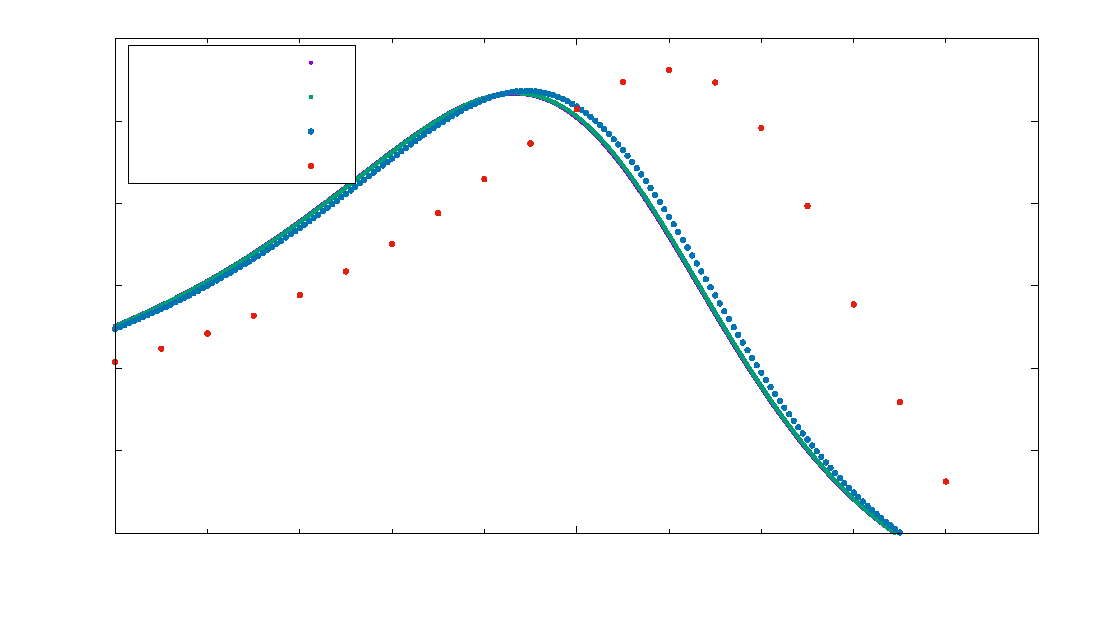
\includegraphics[width={510.20bp},height={283.40bp}]{ConfrPZ}}%
    \gplfronttext
  \end{picture}%
\endgroup

\end{figure}
Infine confrontiamo le traiettorie nello spazio delle fasi:
\begin{figure}[H]
	\centering
	\scalebox{0.9}{% GNUPLOT: LaTeX picture with Postscript
\begingroup
  % Encoding inside the plot.  In the header of your document, this encoding
  % should to defined, e.g., by using
  % \usepackage[cp1252,<other encodings>]{inputenc}
  \inputencoding{cp1252}%
  \makeatletter
  \providecommand\color[2][]{%
    \GenericError{(gnuplot) \space\space\space\@spaces}{%
      Package color not loaded in conjunction with
      terminal option `colourtext'%
    }{See the gnuplot documentation for explanation.%
    }{Either use 'blacktext' in gnuplot or load the package
      color.sty in LaTeX.}%
    \renewcommand\color[2][]{}%
  }%
  \providecommand\includegraphics[2][]{%
    \GenericError{(gnuplot) \space\space\space\@spaces}{%
      Package graphicx or graphics not loaded%
    }{See the gnuplot documentation for explanation.%
    }{The gnuplot epslatex terminal needs graphicx.sty or graphics.sty.}%
    \renewcommand\includegraphics[2][]{}%
  }%
  \providecommand\rotatebox[2]{#2}%
  \@ifundefined{ifGPcolor}{%
    \newif\ifGPcolor
    \GPcolortrue
  }{}%
  \@ifundefined{ifGPblacktext}{%
    \newif\ifGPblacktext
    \GPblacktextfalse
  }{}%
  % define a \g@addto@macro without @ in the name:
  \let\gplgaddtomacro\g@addto@macro
  % define empty templates for all commands taking text:
  \gdef\gplbacktext{}%
  \gdef\gplfronttext{}%
  \makeatother
  \ifGPblacktext
    % no textcolor at all
    \def\colorrgb#1{}%
    \def\colorgray#1{}%
  \else
    % gray or color?
    \ifGPcolor
      \def\colorrgb#1{\color[rgb]{#1}}%
      \def\colorgray#1{\color[gray]{#1}}%
      \expandafter\def\csname LTw\endcsname{\color{white}}%
      \expandafter\def\csname LTb\endcsname{\color{black}}%
      \expandafter\def\csname LTa\endcsname{\color{black}}%
      \expandafter\def\csname LT0\endcsname{\color[rgb]{1,0,0}}%
      \expandafter\def\csname LT1\endcsname{\color[rgb]{0,1,0}}%
      \expandafter\def\csname LT2\endcsname{\color[rgb]{0,0,1}}%
      \expandafter\def\csname LT3\endcsname{\color[rgb]{1,0,1}}%
      \expandafter\def\csname LT4\endcsname{\color[rgb]{0,1,1}}%
      \expandafter\def\csname LT5\endcsname{\color[rgb]{1,1,0}}%
      \expandafter\def\csname LT6\endcsname{\color[rgb]{0,0,0}}%
      \expandafter\def\csname LT7\endcsname{\color[rgb]{1,0.3,0}}%
      \expandafter\def\csname LT8\endcsname{\color[rgb]{0.5,0.5,0.5}}%
    \else
      % gray
      \def\colorrgb#1{\color{black}}%
      \def\colorgray#1{\color[gray]{#1}}%
      \expandafter\def\csname LTw\endcsname{\color{white}}%
      \expandafter\def\csname LTb\endcsname{\color{black}}%
      \expandafter\def\csname LTa\endcsname{\color{black}}%
      \expandafter\def\csname LT0\endcsname{\color{black}}%
      \expandafter\def\csname LT1\endcsname{\color{black}}%
      \expandafter\def\csname LT2\endcsname{\color{black}}%
      \expandafter\def\csname LT3\endcsname{\color{black}}%
      \expandafter\def\csname LT4\endcsname{\color{black}}%
      \expandafter\def\csname LT5\endcsname{\color{black}}%
      \expandafter\def\csname LT6\endcsname{\color{black}}%
      \expandafter\def\csname LT7\endcsname{\color{black}}%
      \expandafter\def\csname LT8\endcsname{\color{black}}%
    \fi
  \fi
    \setlength{\unitlength}{0.0500bp}%
    \ifx\gptboxheight\undefined%
      \newlength{\gptboxheight}%
      \newlength{\gptboxwidth}%
      \newsavebox{\gptboxtext}%
    \fi%
    \setlength{\fboxrule}{0.5pt}%
    \setlength{\fboxsep}{1pt}%
    \definecolor{tbcol}{rgb}{1,1,1}%
\begin{picture}(6802.00,6802.00)%
    \gplgaddtomacro\gplbacktext{%
      \csname LTb\endcsname%%
      \put(682,704){\makebox(0,0)[r]{\strut{}$-3$}}%
      \put(682,1684){\makebox(0,0)[r]{\strut{}$-2$}}%
      \put(682,2663){\makebox(0,0)[r]{\strut{}$-1$}}%
      \put(682,3643){\makebox(0,0)[r]{\strut{}$0$}}%
      \put(682,4622){\makebox(0,0)[r]{\strut{}$1$}}%
      \put(682,5601){\makebox(0,0)[r]{\strut{}$2$}}%
      \put(682,6581){\makebox(0,0)[r]{\strut{}$3$}}%
      \put(814,484){\makebox(0,0){\strut{}$-2.5$}}%
      \put(1373,484){\makebox(0,0){\strut{}$-2$}}%
      \put(1932,484){\makebox(0,0){\strut{}$-1.5$}}%
      \put(2491,484){\makebox(0,0){\strut{}$-1$}}%
      \put(3050,484){\makebox(0,0){\strut{}$-0.5$}}%
      \put(3610,484){\makebox(0,0){\strut{}$0$}}%
      \put(4169,484){\makebox(0,0){\strut{}$0.5$}}%
      \put(4728,484){\makebox(0,0){\strut{}$1$}}%
      \put(5287,484){\makebox(0,0){\strut{}$1.5$}}%
      \put(5846,484){\makebox(0,0){\strut{}$2$}}%
      \put(6405,484){\makebox(0,0){\strut{}$2.5$}}%
    }%
    \gplgaddtomacro\gplfronttext{%
      \csname LTb\endcsname%%
      \put(209,3642){\rotatebox{-270}{\makebox(0,0){\strut{}p}}}%
      \put(3609,154){\makebox(0,0){\strut{}x}}%
      \csname LTb\endcsname%%
      \put(2266,6353){\makebox(0,0)[r]{\strut{}$h = 0.0001$}}%
      \csname LTb\endcsname%%
      \put(2266,6023){\makebox(0,0)[r]{\strut{}$h = 0.001$}}%
      \csname LTb\endcsname%%
      \put(2266,5693){\makebox(0,0)[r]{\strut{}$h = 0.01$}}%
      \csname LTb\endcsname%%
      \put(2266,5363){\makebox(0,0)[r]{\strut{}$h = 0.1$}}%
    }%
    \gplbacktext
    \put(0,0){\includegraphics[width={340.10bp},height={340.10bp}]{ConfrMu1}}%
    \gplfronttext
  \end{picture}%
\endgroup
}
\end{figure}
e vediamo che, nonostante per $\Delta t = 0.1$ la traiettoria sia piuttosto diversa da quella "esatta", per gli altri time step si ottengono delle traiettorie molto simili. \\ \\
A questo punto possiamo anche calcolare l'ordine di accuratezza delle soluzioni come accennato nella sezione precedente. 
Come detto in precedenza per calcolare l'accuratezza di una soluzione numerica di un'equazione differenziale bisogna posizionarsi in uno spazio normato di funzioni e scegliere la norma in modo adeguato, per poi calcolare la distanza tra la soluzione approssimata e quella esatta nella metrica indotta. \\
In questo caso si è scelta la norma
\begin{equation}
	||f(x)|| = \max_x |f(x)|
\end{equation}
che induce la metrica
\begin{equation}
	||f(x) - g(x)|| = \max_x |f(x) - g(x)|
\end{equation} \\
A questo punto possiamo quindi definire la funzione di errore
\begin{equation}
	E(h) = ||v - v_h|| = \max_x |v - v_h| \leq Ch^n
\end{equation}
dove $h$ è il timestep e $n$ è l'ordine di accuratezza. \\ \\
Per le tre soluzioni citate in precedenza è stato calcolato l'errore mediante un codice che calcola la distanza tra le soluzioni $x(t)$, e questo calcolo è stato fatto confrontando i valori di $x$ a parità di valori di $n$. \\
Per le tre soluzioni si sono ottenuti i seguenti errori:
\begin{equation}
	E(h = 0.1) = 2.04 \ \ \ \ \ \ \ \ \ \  E(h = 0.01) = 0.19  \ \ \ \ \ \ \ \ \ \ E(h = 0.001) = 0.017
\end{equation}
e si nota che questi errori sono consistenti con un'accuratezza di ordine $1$, perchè vediamo che se $h$ diminuisce di un ordine di grandezza, l'errore fa lo stesso.
\subsubsection{Confronto sulla rigidità per $\mu = 10$}
Vogliamo ora confrontare di nuovo le soluzioni approssimate, ma prendendo l'equazione con una costante di smorzamento, e quindi una rigidità, dieci vole maggiore. I timestep utilizzati e che mettiamo a confronto sono $h=0.01$, $h=0.001$, $h=0.0001$ e $h=0.00005$. Similmente a prima, confrontando gli andamenti temporali di $x(t)$ vediamo che per $h = 0.00005$ e $h = 0.0001$ otteniamo delle soluzioni quasi completamente sovrapposte, per $h = 0.001$ ovveniamo una soluzione che si discosta leggermente dalle prime due, mentre con $h = 0.01$ otteniamo una soluzione che si discosta enormemente dalle altre, ed è quindi inadeguata a risolvere l'equazione in maniera soddisfacente.
\begin{figure}[H]
	\centering
	% GNUPLOT: LaTeX picture with Postscript
\begingroup
  % Encoding inside the plot.  In the header of your document, this encoding
  % should to defined, e.g., by using
  % \usepackage[cp1252,<other encodings>]{inputenc}
  \inputencoding{cp1252}%
  \makeatletter
  \providecommand\color[2][]{%
    \GenericError{(gnuplot) \space\space\space\@spaces}{%
      Package color not loaded in conjunction with
      terminal option `colourtext'%
    }{See the gnuplot documentation for explanation.%
    }{Either use 'blacktext' in gnuplot or load the package
      color.sty in LaTeX.}%
    \renewcommand\color[2][]{}%
  }%
  \providecommand\includegraphics[2][]{%
    \GenericError{(gnuplot) \space\space\space\@spaces}{%
      Package graphicx or graphics not loaded%
    }{See the gnuplot documentation for explanation.%
    }{The gnuplot epslatex terminal needs graphicx.sty or graphics.sty.}%
    \renewcommand\includegraphics[2][]{}%
  }%
  \providecommand\rotatebox[2]{#2}%
  \@ifundefined{ifGPcolor}{%
    \newif\ifGPcolor
    \GPcolortrue
  }{}%
  \@ifundefined{ifGPblacktext}{%
    \newif\ifGPblacktext
    \GPblacktextfalse
  }{}%
  % define a \g@addto@macro without @ in the name:
  \let\gplgaddtomacro\g@addto@macro
  % define empty templates for all commands taking text:
  \gdef\gplbacktext{}%
  \gdef\gplfronttext{}%
  \makeatother
  \ifGPblacktext
    % no textcolor at all
    \def\colorrgb#1{}%
    \def\colorgray#1{}%
  \else
    % gray or color?
    \ifGPcolor
      \def\colorrgb#1{\color[rgb]{#1}}%
      \def\colorgray#1{\color[gray]{#1}}%
      \expandafter\def\csname LTw\endcsname{\color{white}}%
      \expandafter\def\csname LTb\endcsname{\color{black}}%
      \expandafter\def\csname LTa\endcsname{\color{black}}%
      \expandafter\def\csname LT0\endcsname{\color[rgb]{1,0,0}}%
      \expandafter\def\csname LT1\endcsname{\color[rgb]{0,1,0}}%
      \expandafter\def\csname LT2\endcsname{\color[rgb]{0,0,1}}%
      \expandafter\def\csname LT3\endcsname{\color[rgb]{1,0,1}}%
      \expandafter\def\csname LT4\endcsname{\color[rgb]{0,1,1}}%
      \expandafter\def\csname LT5\endcsname{\color[rgb]{1,1,0}}%
      \expandafter\def\csname LT6\endcsname{\color[rgb]{0,0,0}}%
      \expandafter\def\csname LT7\endcsname{\color[rgb]{1,0.3,0}}%
      \expandafter\def\csname LT8\endcsname{\color[rgb]{0.5,0.5,0.5}}%
    \else
      % gray
      \def\colorrgb#1{\color{black}}%
      \def\colorgray#1{\color[gray]{#1}}%
      \expandafter\def\csname LTw\endcsname{\color{white}}%
      \expandafter\def\csname LTb\endcsname{\color{black}}%
      \expandafter\def\csname LTa\endcsname{\color{black}}%
      \expandafter\def\csname LT0\endcsname{\color{black}}%
      \expandafter\def\csname LT1\endcsname{\color{black}}%
      \expandafter\def\csname LT2\endcsname{\color{black}}%
      \expandafter\def\csname LT3\endcsname{\color{black}}%
      \expandafter\def\csname LT4\endcsname{\color{black}}%
      \expandafter\def\csname LT5\endcsname{\color{black}}%
      \expandafter\def\csname LT6\endcsname{\color{black}}%
      \expandafter\def\csname LT7\endcsname{\color{black}}%
      \expandafter\def\csname LT8\endcsname{\color{black}}%
    \fi
  \fi
    \setlength{\unitlength}{0.0500bp}%
    \ifx\gptboxheight\undefined%
      \newlength{\gptboxheight}%
      \newlength{\gptboxwidth}%
      \newsavebox{\gptboxtext}%
    \fi%
    \setlength{\fboxrule}{0.5pt}%
    \setlength{\fboxsep}{1pt}%
    \definecolor{tbcol}{rgb}{1,1,1}%
\begin{picture}(9070.00,5668.00)%
    \gplgaddtomacro\gplbacktext{%
      \csname LTb\endcsname%%
      \put(946,1178){\makebox(0,0)[r]{\strut{}$-2$}}%
      \put(946,1653){\makebox(0,0)[r]{\strut{}$-1.5$}}%
      \put(946,2127){\makebox(0,0)[r]{\strut{}$-1$}}%
      \put(946,2601){\makebox(0,0)[r]{\strut{}$-0.5$}}%
      \put(946,3076){\makebox(0,0)[r]{\strut{}$0$}}%
      \put(946,3550){\makebox(0,0)[r]{\strut{}$0.5$}}%
      \put(946,4024){\makebox(0,0)[r]{\strut{}$1$}}%
      \put(946,4498){\makebox(0,0)[r]{\strut{}$1.5$}}%
      \put(946,4973){\makebox(0,0)[r]{\strut{}$2$}}%
      \put(1078,484){\makebox(0,0){\strut{}$0$}}%
      \put(1838,484){\makebox(0,0){\strut{}$2.5$}}%
      \put(2597,484){\makebox(0,0){\strut{}$5$}}%
      \put(3357,484){\makebox(0,0){\strut{}$7.5$}}%
      \put(4116,484){\makebox(0,0){\strut{}$10$}}%
      \put(4876,484){\makebox(0,0){\strut{}$12.5$}}%
      \put(5635,484){\makebox(0,0){\strut{}$15$}}%
      \put(6395,484){\makebox(0,0){\strut{}$17.5$}}%
      \put(7154,484){\makebox(0,0){\strut{}$20$}}%
      \put(7914,484){\makebox(0,0){\strut{}$22.5$}}%
      \put(8673,484){\makebox(0,0){\strut{}$25$}}%
    }%
    \gplgaddtomacro\gplfronttext{%
      \csname LTb\endcsname%%
      \put(209,3075){\rotatebox{-270}{\makebox(0,0){\strut{}x(t)}}}%
      \put(4875,154){\makebox(0,0){\strut{}t}}%
      \csname LTb\endcsname%%
      \put(2662,5219){\makebox(0,0)[r]{\strut{}$h = 0.0001$}}%
      \csname LTb\endcsname%%
      \put(2662,4889){\makebox(0,0)[r]{\strut{}$h = 0.001$}}%
      \csname LTb\endcsname%%
      \put(2662,4559){\makebox(0,0)[r]{\strut{}$h = 0.01$}}%
      \csname LTb\endcsname%%
      \put(2662,4229){\makebox(0,0)[r]{\strut{}$h = 0.00005$}}%
    }%
    \gplbacktext
    \put(0,0){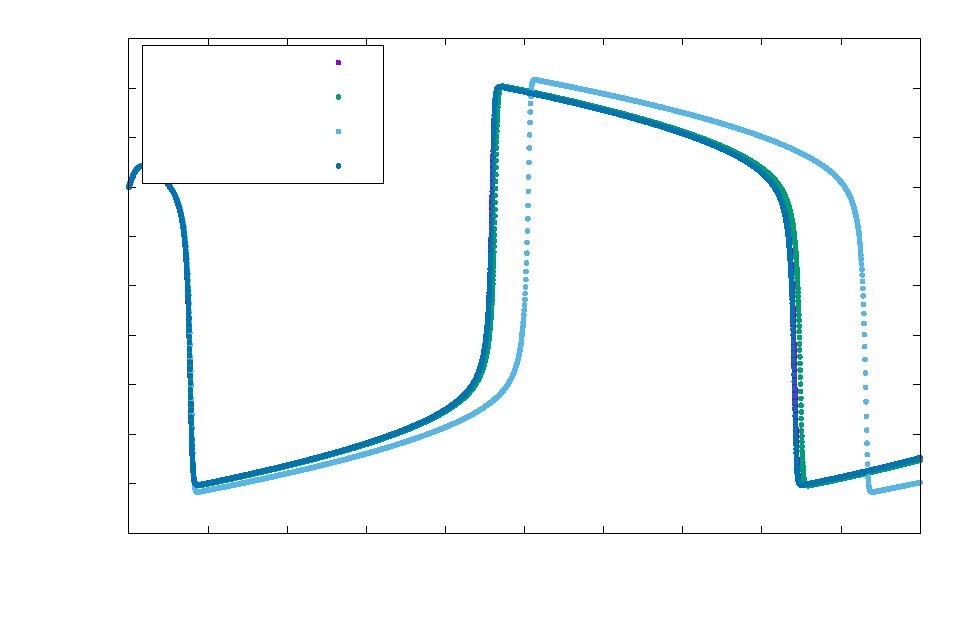
\includegraphics[width={453.50bp},height={283.40bp}]{Comp10X}}%
    \gplfronttext
  \end{picture}%
\endgroup

\end{figure}
Se ora zoomiamo in una piccola regione del grafico vediamo che effettivamente la curva viola e quella blu, corrispondenti a $h = 0.0001$ e $h = 0.00005$ sono quasi indistinguibili. 
\begin{figure}[H]
	\centering
	% GNUPLOT: LaTeX picture with Postscript
\begingroup
  % Encoding inside the plot.  In the header of your document, this encoding
  % should to defined, e.g., by using
  % \usepackage[cp1252,<other encodings>]{inputenc}
  \inputencoding{cp1252}%
  \makeatletter
  \providecommand\color[2][]{%
    \GenericError{(gnuplot) \space\space\space\@spaces}{%
      Package color not loaded in conjunction with
      terminal option `colourtext'%
    }{See the gnuplot documentation for explanation.%
    }{Either use 'blacktext' in gnuplot or load the package
      color.sty in LaTeX.}%
    \renewcommand\color[2][]{}%
  }%
  \providecommand\includegraphics[2][]{%
    \GenericError{(gnuplot) \space\space\space\@spaces}{%
      Package graphicx or graphics not loaded%
    }{See the gnuplot documentation for explanation.%
    }{The gnuplot epslatex terminal needs graphicx.sty or graphics.sty.}%
    \renewcommand\includegraphics[2][]{}%
  }%
  \providecommand\rotatebox[2]{#2}%
  \@ifundefined{ifGPcolor}{%
    \newif\ifGPcolor
    \GPcolortrue
  }{}%
  \@ifundefined{ifGPblacktext}{%
    \newif\ifGPblacktext
    \GPblacktextfalse
  }{}%
  % define a \g@addto@macro without @ in the name:
  \let\gplgaddtomacro\g@addto@macro
  % define empty templates for all commands taking text:
  \gdef\gplbacktext{}%
  \gdef\gplfronttext{}%
  \makeatother
  \ifGPblacktext
    % no textcolor at all
    \def\colorrgb#1{}%
    \def\colorgray#1{}%
  \else
    % gray or color?
    \ifGPcolor
      \def\colorrgb#1{\color[rgb]{#1}}%
      \def\colorgray#1{\color[gray]{#1}}%
      \expandafter\def\csname LTw\endcsname{\color{white}}%
      \expandafter\def\csname LTb\endcsname{\color{black}}%
      \expandafter\def\csname LTa\endcsname{\color{black}}%
      \expandafter\def\csname LT0\endcsname{\color[rgb]{1,0,0}}%
      \expandafter\def\csname LT1\endcsname{\color[rgb]{0,1,0}}%
      \expandafter\def\csname LT2\endcsname{\color[rgb]{0,0,1}}%
      \expandafter\def\csname LT3\endcsname{\color[rgb]{1,0,1}}%
      \expandafter\def\csname LT4\endcsname{\color[rgb]{0,1,1}}%
      \expandafter\def\csname LT5\endcsname{\color[rgb]{1,1,0}}%
      \expandafter\def\csname LT6\endcsname{\color[rgb]{0,0,0}}%
      \expandafter\def\csname LT7\endcsname{\color[rgb]{1,0.3,0}}%
      \expandafter\def\csname LT8\endcsname{\color[rgb]{0.5,0.5,0.5}}%
    \else
      % gray
      \def\colorrgb#1{\color{black}}%
      \def\colorgray#1{\color[gray]{#1}}%
      \expandafter\def\csname LTw\endcsname{\color{white}}%
      \expandafter\def\csname LTb\endcsname{\color{black}}%
      \expandafter\def\csname LTa\endcsname{\color{black}}%
      \expandafter\def\csname LT0\endcsname{\color{black}}%
      \expandafter\def\csname LT1\endcsname{\color{black}}%
      \expandafter\def\csname LT2\endcsname{\color{black}}%
      \expandafter\def\csname LT3\endcsname{\color{black}}%
      \expandafter\def\csname LT4\endcsname{\color{black}}%
      \expandafter\def\csname LT5\endcsname{\color{black}}%
      \expandafter\def\csname LT6\endcsname{\color{black}}%
      \expandafter\def\csname LT7\endcsname{\color{black}}%
      \expandafter\def\csname LT8\endcsname{\color{black}}%
    \fi
  \fi
    \setlength{\unitlength}{0.0500bp}%
    \ifx\gptboxheight\undefined%
      \newlength{\gptboxheight}%
      \newlength{\gptboxwidth}%
      \newsavebox{\gptboxtext}%
    \fi%
    \setlength{\fboxrule}{0.5pt}%
    \setlength{\fboxsep}{1pt}%
    \definecolor{tbcol}{rgb}{1,1,1}%
\begin{picture}(9070.00,5668.00)%
    \gplgaddtomacro\gplbacktext{%
      \csname LTb\endcsname%%
      \put(814,704){\makebox(0,0)[r]{\strut{}$1$}}%
      \put(814,2680){\makebox(0,0)[r]{\strut{}$1.5$}}%
      \put(814,4657){\makebox(0,0)[r]{\strut{}$2$}}%
      \put(2234,484){\makebox(0,0){\strut{}$12.5$}}%
      \put(4380,484){\makebox(0,0){\strut{}$15$}}%
      \put(6527,484){\makebox(0,0){\strut{}$17.5$}}%
      \put(8673,484){\makebox(0,0){\strut{}$20$}}%
    }%
    \gplgaddtomacro\gplfronttext{%
      \csname LTb\endcsname%%
      \put(209,3075){\rotatebox{-270}{\makebox(0,0){\strut{}x(t)}}}%
      \put(4809,154){\makebox(0,0){\strut{}t}}%
      \csname LTb\endcsname%%
      \put(7686,5219){\makebox(0,0)[r]{\strut{}$h = 0.0001$}}%
      \csname LTb\endcsname%%
      \put(7686,4889){\makebox(0,0)[r]{\strut{}$h = 0.001$}}%
      \csname LTb\endcsname%%
      \put(7686,4559){\makebox(0,0)[r]{\strut{}$h = 0.01$}}%
      \csname LTb\endcsname%%
      \put(7686,4229){\makebox(0,0)[r]{\strut{}$h = 0.00005$}}%
    }%
    \gplbacktext
    \put(0,0){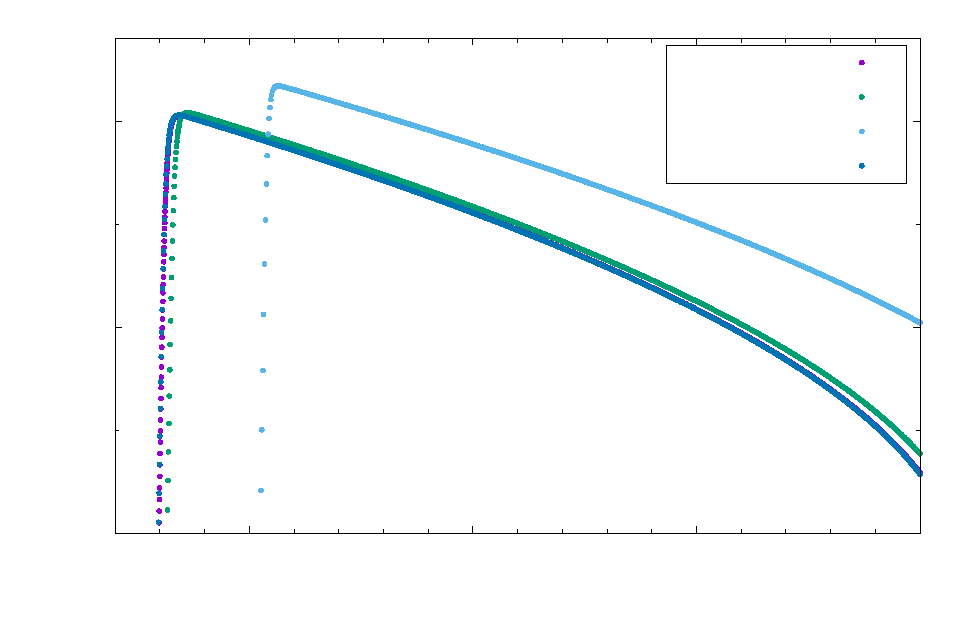
\includegraphics[width={453.50bp},height={283.40bp}]{Comp10XZ}}%
    \gplfronttext
  \end{picture}%
\endgroup

\end{figure}
Ora effettuamiamo lo stesso confronto per gli andamenti temporali degli impulsi $p(t)$
e vediamo che valgono le stesse considerazioni appena fatte per l'andamento di $x(t)$. 
\begin{figure}[H]
	\centering
	% GNUPLOT: LaTeX picture with Postscript
\begingroup
  % Encoding inside the plot.  In the header of your document, this encoding
  % should to defined, e.g., by using
  % \usepackage[cp1252,<other encodings>]{inputenc}
  \inputencoding{cp1252}%
  \makeatletter
  \providecommand\color[2][]{%
    \GenericError{(gnuplot) \space\space\space\@spaces}{%
      Package color not loaded in conjunction with
      terminal option `colourtext'%
    }{See the gnuplot documentation for explanation.%
    }{Either use 'blacktext' in gnuplot or load the package
      color.sty in LaTeX.}%
    \renewcommand\color[2][]{}%
  }%
  \providecommand\includegraphics[2][]{%
    \GenericError{(gnuplot) \space\space\space\@spaces}{%
      Package graphicx or graphics not loaded%
    }{See the gnuplot documentation for explanation.%
    }{The gnuplot epslatex terminal needs graphicx.sty or graphics.sty.}%
    \renewcommand\includegraphics[2][]{}%
  }%
  \providecommand\rotatebox[2]{#2}%
  \@ifundefined{ifGPcolor}{%
    \newif\ifGPcolor
    \GPcolortrue
  }{}%
  \@ifundefined{ifGPblacktext}{%
    \newif\ifGPblacktext
    \GPblacktextfalse
  }{}%
  % define a \g@addto@macro without @ in the name:
  \let\gplgaddtomacro\g@addto@macro
  % define empty templates for all commands taking text:
  \gdef\gplbacktext{}%
  \gdef\gplfronttext{}%
  \makeatother
  \ifGPblacktext
    % no textcolor at all
    \def\colorrgb#1{}%
    \def\colorgray#1{}%
  \else
    % gray or color?
    \ifGPcolor
      \def\colorrgb#1{\color[rgb]{#1}}%
      \def\colorgray#1{\color[gray]{#1}}%
      \expandafter\def\csname LTw\endcsname{\color{white}}%
      \expandafter\def\csname LTb\endcsname{\color{black}}%
      \expandafter\def\csname LTa\endcsname{\color{black}}%
      \expandafter\def\csname LT0\endcsname{\color[rgb]{1,0,0}}%
      \expandafter\def\csname LT1\endcsname{\color[rgb]{0,1,0}}%
      \expandafter\def\csname LT2\endcsname{\color[rgb]{0,0,1}}%
      \expandafter\def\csname LT3\endcsname{\color[rgb]{1,0,1}}%
      \expandafter\def\csname LT4\endcsname{\color[rgb]{0,1,1}}%
      \expandafter\def\csname LT5\endcsname{\color[rgb]{1,1,0}}%
      \expandafter\def\csname LT6\endcsname{\color[rgb]{0,0,0}}%
      \expandafter\def\csname LT7\endcsname{\color[rgb]{1,0.3,0}}%
      \expandafter\def\csname LT8\endcsname{\color[rgb]{0.5,0.5,0.5}}%
    \else
      % gray
      \def\colorrgb#1{\color{black}}%
      \def\colorgray#1{\color[gray]{#1}}%
      \expandafter\def\csname LTw\endcsname{\color{white}}%
      \expandafter\def\csname LTb\endcsname{\color{black}}%
      \expandafter\def\csname LTa\endcsname{\color{black}}%
      \expandafter\def\csname LT0\endcsname{\color{black}}%
      \expandafter\def\csname LT1\endcsname{\color{black}}%
      \expandafter\def\csname LT2\endcsname{\color{black}}%
      \expandafter\def\csname LT3\endcsname{\color{black}}%
      \expandafter\def\csname LT4\endcsname{\color{black}}%
      \expandafter\def\csname LT5\endcsname{\color{black}}%
      \expandafter\def\csname LT6\endcsname{\color{black}}%
      \expandafter\def\csname LT7\endcsname{\color{black}}%
      \expandafter\def\csname LT8\endcsname{\color{black}}%
    \fi
  \fi
    \setlength{\unitlength}{0.0500bp}%
    \ifx\gptboxheight\undefined%
      \newlength{\gptboxheight}%
      \newlength{\gptboxwidth}%
      \newsavebox{\gptboxtext}%
    \fi%
    \setlength{\fboxrule}{0.5pt}%
    \setlength{\fboxsep}{1pt}%
    \definecolor{tbcol}{rgb}{1,1,1}%
\begin{picture}(10204.00,5668.00)%
    \gplgaddtomacro\gplbacktext{%
      \csname LTb\endcsname%%
      \put(814,1466){\makebox(0,0)[r]{\strut{}$-10$}}%
      \put(814,2270){\makebox(0,0)[r]{\strut{}$-5$}}%
      \put(814,3075){\makebox(0,0)[r]{\strut{}$0$}}%
      \put(814,3879){\makebox(0,0)[r]{\strut{}$5$}}%
      \put(814,4683){\makebox(0,0)[r]{\strut{}$10$}}%
      \put(946,484){\makebox(0,0){\strut{}$0$}}%
      \put(1832,484){\makebox(0,0){\strut{}$2.5$}}%
      \put(2718,484){\makebox(0,0){\strut{}$5$}}%
      \put(3604,484){\makebox(0,0){\strut{}$7.5$}}%
      \put(4490,484){\makebox(0,0){\strut{}$10$}}%
      \put(5377,484){\makebox(0,0){\strut{}$12.5$}}%
      \put(6263,484){\makebox(0,0){\strut{}$15$}}%
      \put(7149,484){\makebox(0,0){\strut{}$17.5$}}%
      \put(8035,484){\makebox(0,0){\strut{}$20$}}%
      \put(8921,484){\makebox(0,0){\strut{}$22.5$}}%
      \put(9807,484){\makebox(0,0){\strut{}$25$}}%
    }%
    \gplgaddtomacro\gplfronttext{%
      \csname LTb\endcsname%%
      \put(209,3075){\rotatebox{-270}{\makebox(0,0){\strut{}x(t)}}}%
      \put(5376,154){\makebox(0,0){\strut{}t}}%
      \csname LTb\endcsname%%
      \put(2530,5219){\makebox(0,0)[r]{\strut{}$h = 0.0001$}}%
      \csname LTb\endcsname%%
      \put(2530,4889){\makebox(0,0)[r]{\strut{}$h = 0.001$}}%
      \csname LTb\endcsname%%
      \put(2530,4559){\makebox(0,0)[r]{\strut{}$h = 0.01$}}%
      \csname LTb\endcsname%%
      \put(2530,4229){\makebox(0,0)[r]{\strut{}$h = 0.00005$}}%
    }%
    \gplbacktext
    \put(0,0){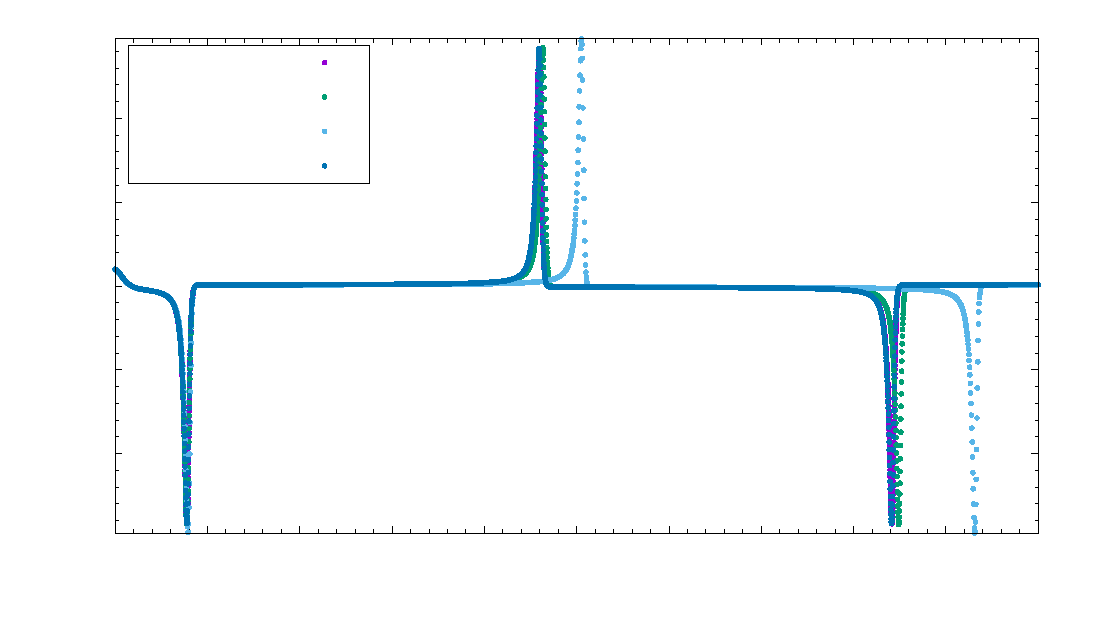
\includegraphics[width={510.20bp},height={283.40bp}]{Comp10PZ}}%
    \gplfronttext
  \end{picture}%
\endgroup

\end{figure}
Se come prima effettuiamo uno zoom vediamo che le curve con $h = 0.0001$ e $h = 0.00005$ sono quasi indistinguibili.
\begin{figure}[H]
	\centering
	% GNUPLOT: LaTeX picture with Postscript
\begingroup
  % Encoding inside the plot.  In the header of your document, this encoding
  % should to defined, e.g., by using
  % \usepackage[cp1252,<other encodings>]{inputenc}
  \inputencoding{cp1252}%
  \makeatletter
  \providecommand\color[2][]{%
    \GenericError{(gnuplot) \space\space\space\@spaces}{%
      Package color not loaded in conjunction with
      terminal option `colourtext'%
    }{See the gnuplot documentation for explanation.%
    }{Either use 'blacktext' in gnuplot or load the package
      color.sty in LaTeX.}%
    \renewcommand\color[2][]{}%
  }%
  \providecommand\includegraphics[2][]{%
    \GenericError{(gnuplot) \space\space\space\@spaces}{%
      Package graphicx or graphics not loaded%
    }{See the gnuplot documentation for explanation.%
    }{The gnuplot epslatex terminal needs graphicx.sty or graphics.sty.}%
    \renewcommand\includegraphics[2][]{}%
  }%
  \providecommand\rotatebox[2]{#2}%
  \@ifundefined{ifGPcolor}{%
    \newif\ifGPcolor
    \GPcolortrue
  }{}%
  \@ifundefined{ifGPblacktext}{%
    \newif\ifGPblacktext
    \GPblacktextfalse
  }{}%
  % define a \g@addto@macro without @ in the name:
  \let\gplgaddtomacro\g@addto@macro
  % define empty templates for all commands taking text:
  \gdef\gplbacktext{}%
  \gdef\gplfronttext{}%
  \makeatother
  \ifGPblacktext
    % no textcolor at all
    \def\colorrgb#1{}%
    \def\colorgray#1{}%
  \else
    % gray or color?
    \ifGPcolor
      \def\colorrgb#1{\color[rgb]{#1}}%
      \def\colorgray#1{\color[gray]{#1}}%
      \expandafter\def\csname LTw\endcsname{\color{white}}%
      \expandafter\def\csname LTb\endcsname{\color{black}}%
      \expandafter\def\csname LTa\endcsname{\color{black}}%
      \expandafter\def\csname LT0\endcsname{\color[rgb]{1,0,0}}%
      \expandafter\def\csname LT1\endcsname{\color[rgb]{0,1,0}}%
      \expandafter\def\csname LT2\endcsname{\color[rgb]{0,0,1}}%
      \expandafter\def\csname LT3\endcsname{\color[rgb]{1,0,1}}%
      \expandafter\def\csname LT4\endcsname{\color[rgb]{0,1,1}}%
      \expandafter\def\csname LT5\endcsname{\color[rgb]{1,1,0}}%
      \expandafter\def\csname LT6\endcsname{\color[rgb]{0,0,0}}%
      \expandafter\def\csname LT7\endcsname{\color[rgb]{1,0.3,0}}%
      \expandafter\def\csname LT8\endcsname{\color[rgb]{0.5,0.5,0.5}}%
    \else
      % gray
      \def\colorrgb#1{\color{black}}%
      \def\colorgray#1{\color[gray]{#1}}%
      \expandafter\def\csname LTw\endcsname{\color{white}}%
      \expandafter\def\csname LTb\endcsname{\color{black}}%
      \expandafter\def\csname LTa\endcsname{\color{black}}%
      \expandafter\def\csname LT0\endcsname{\color{black}}%
      \expandafter\def\csname LT1\endcsname{\color{black}}%
      \expandafter\def\csname LT2\endcsname{\color{black}}%
      \expandafter\def\csname LT3\endcsname{\color{black}}%
      \expandafter\def\csname LT4\endcsname{\color{black}}%
      \expandafter\def\csname LT5\endcsname{\color{black}}%
      \expandafter\def\csname LT6\endcsname{\color{black}}%
      \expandafter\def\csname LT7\endcsname{\color{black}}%
      \expandafter\def\csname LT8\endcsname{\color{black}}%
    \fi
  \fi
    \setlength{\unitlength}{0.0500bp}%
    \ifx\gptboxheight\undefined%
      \newlength{\gptboxheight}%
      \newlength{\gptboxwidth}%
      \newsavebox{\gptboxtext}%
    \fi%
    \setlength{\fboxrule}{0.5pt}%
    \setlength{\fboxsep}{1pt}%
    \definecolor{tbcol}{rgb}{1,1,1}%
\begin{picture}(10204.00,5668.00)%
    \gplgaddtomacro\gplbacktext{%
      \csname LTb\endcsname%%
      \put(682,1000){\makebox(0,0)[r]{\strut{}$0$}}%
      \put(682,2483){\makebox(0,0)[r]{\strut{}$5$}}%
      \put(682,3965){\makebox(0,0)[r]{\strut{}$10$}}%
      \put(682,5447){\makebox(0,0)[r]{\strut{}$15$}}%
      \put(814,484){\makebox(0,0){\strut{}$10$}}%
      \put(2313,484){\makebox(0,0){\strut{}$10.5$}}%
      \put(3812,484){\makebox(0,0){\strut{}$11$}}%
      \put(5311,484){\makebox(0,0){\strut{}$11.5$}}%
      \put(6809,484){\makebox(0,0){\strut{}$12$}}%
      \put(8308,484){\makebox(0,0){\strut{}$12.5$}}%
      \put(9807,484){\makebox(0,0){\strut{}$13$}}%
    }%
    \gplgaddtomacro\gplfronttext{%
      \csname LTb\endcsname%%
      \put(209,3075){\rotatebox{-270}{\makebox(0,0){\strut{}x(t)}}}%
      \put(5310,154){\makebox(0,0){\strut{}t}}%
      \csname LTb\endcsname%%
      \put(2398,5219){\makebox(0,0)[r]{\strut{}$h = 0.0001$}}%
      \csname LTb\endcsname%%
      \put(2398,4889){\makebox(0,0)[r]{\strut{}$h = 0.001$}}%
      \csname LTb\endcsname%%
      \put(2398,4559){\makebox(0,0)[r]{\strut{}$h = 0.01$}}%
      \csname LTb\endcsname%%
      \put(2398,4229){\makebox(0,0)[r]{\strut{}$h = 0.00005$}}%
    }%
    \gplbacktext
    \put(0,0){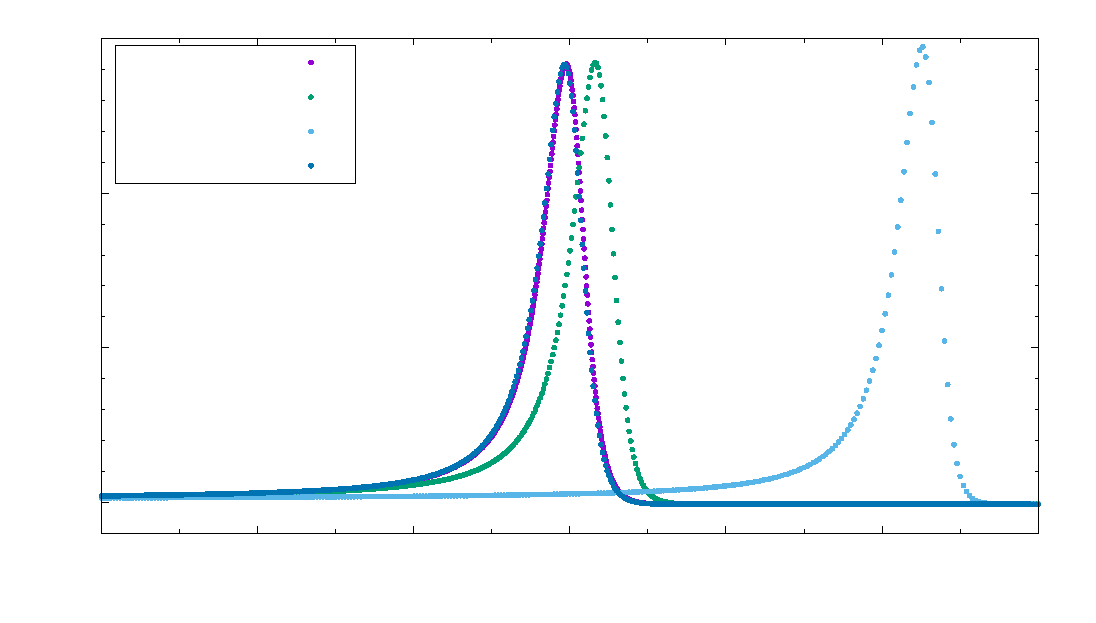
\includegraphics[width={510.20bp},height={283.40bp}]{Comp10PZZ}}%
    \gplfronttext
  \end{picture}%
\endgroup

\end{figure}
Infine confrontiamo le traiettorie nello spazio delle fasi:
\begin{figure}[H]
	\centering
	% GNUPLOT: LaTeX picture with Postscript
\begingroup
  % Encoding inside the plot.  In the header of your document, this encoding
  % should to defined, e.g., by using
  % \usepackage[cp1252,<other encodings>]{inputenc}
  \inputencoding{cp1252}%
  \makeatletter
  \providecommand\color[2][]{%
    \GenericError{(gnuplot) \space\space\space\@spaces}{%
      Package color not loaded in conjunction with
      terminal option `colourtext'%
    }{See the gnuplot documentation for explanation.%
    }{Either use 'blacktext' in gnuplot or load the package
      color.sty in LaTeX.}%
    \renewcommand\color[2][]{}%
  }%
  \providecommand\includegraphics[2][]{%
    \GenericError{(gnuplot) \space\space\space\@spaces}{%
      Package graphicx or graphics not loaded%
    }{See the gnuplot documentation for explanation.%
    }{The gnuplot epslatex terminal needs graphicx.sty or graphics.sty.}%
    \renewcommand\includegraphics[2][]{}%
  }%
  \providecommand\rotatebox[2]{#2}%
  \@ifundefined{ifGPcolor}{%
    \newif\ifGPcolor
    \GPcolortrue
  }{}%
  \@ifundefined{ifGPblacktext}{%
    \newif\ifGPblacktext
    \GPblacktextfalse
  }{}%
  % define a \g@addto@macro without @ in the name:
  \let\gplgaddtomacro\g@addto@macro
  % define empty templates for all commands taking text:
  \gdef\gplbacktext{}%
  \gdef\gplfronttext{}%
  \makeatother
  \ifGPblacktext
    % no textcolor at all
    \def\colorrgb#1{}%
    \def\colorgray#1{}%
  \else
    % gray or color?
    \ifGPcolor
      \def\colorrgb#1{\color[rgb]{#1}}%
      \def\colorgray#1{\color[gray]{#1}}%
      \expandafter\def\csname LTw\endcsname{\color{white}}%
      \expandafter\def\csname LTb\endcsname{\color{black}}%
      \expandafter\def\csname LTa\endcsname{\color{black}}%
      \expandafter\def\csname LT0\endcsname{\color[rgb]{1,0,0}}%
      \expandafter\def\csname LT1\endcsname{\color[rgb]{0,1,0}}%
      \expandafter\def\csname LT2\endcsname{\color[rgb]{0,0,1}}%
      \expandafter\def\csname LT3\endcsname{\color[rgb]{1,0,1}}%
      \expandafter\def\csname LT4\endcsname{\color[rgb]{0,1,1}}%
      \expandafter\def\csname LT5\endcsname{\color[rgb]{1,1,0}}%
      \expandafter\def\csname LT6\endcsname{\color[rgb]{0,0,0}}%
      \expandafter\def\csname LT7\endcsname{\color[rgb]{1,0.3,0}}%
      \expandafter\def\csname LT8\endcsname{\color[rgb]{0.5,0.5,0.5}}%
    \else
      % gray
      \def\colorrgb#1{\color{black}}%
      \def\colorgray#1{\color[gray]{#1}}%
      \expandafter\def\csname LTw\endcsname{\color{white}}%
      \expandafter\def\csname LTb\endcsname{\color{black}}%
      \expandafter\def\csname LTa\endcsname{\color{black}}%
      \expandafter\def\csname LT0\endcsname{\color{black}}%
      \expandafter\def\csname LT1\endcsname{\color{black}}%
      \expandafter\def\csname LT2\endcsname{\color{black}}%
      \expandafter\def\csname LT3\endcsname{\color{black}}%
      \expandafter\def\csname LT4\endcsname{\color{black}}%
      \expandafter\def\csname LT5\endcsname{\color{black}}%
      \expandafter\def\csname LT6\endcsname{\color{black}}%
      \expandafter\def\csname LT7\endcsname{\color{black}}%
      \expandafter\def\csname LT8\endcsname{\color{black}}%
    \fi
  \fi
    \setlength{\unitlength}{0.0500bp}%
    \ifx\gptboxheight\undefined%
      \newlength{\gptboxheight}%
      \newlength{\gptboxwidth}%
      \newsavebox{\gptboxtext}%
    \fi%
    \setlength{\fboxrule}{0.5pt}%
    \setlength{\fboxsep}{1pt}%
    \definecolor{tbcol}{rgb}{1,1,1}%
\begin{picture}(6802.00,6236.00)%
    \gplgaddtomacro\gplbacktext{%
      \csname LTb\endcsname%%
      \put(814,704){\makebox(0,0)[r]{\strut{}$-15$}}%
      \put(814,1589){\makebox(0,0)[r]{\strut{}$-10$}}%
      \put(814,2474){\makebox(0,0)[r]{\strut{}$-5$}}%
      \put(814,3360){\makebox(0,0)[r]{\strut{}$0$}}%
      \put(814,4245){\makebox(0,0)[r]{\strut{}$5$}}%
      \put(814,5130){\makebox(0,0)[r]{\strut{}$10$}}%
      \put(814,6015){\makebox(0,0)[r]{\strut{}$15$}}%
      \put(946,484){\makebox(0,0){\strut{}$-2.5$}}%
      \put(2038,484){\makebox(0,0){\strut{}$-1.5$}}%
      \put(3130,484){\makebox(0,0){\strut{}$-0.5$}}%
      \put(4221,484){\makebox(0,0){\strut{}$0.5$}}%
      \put(5313,484){\makebox(0,0){\strut{}$1.5$}}%
      \put(6405,484){\makebox(0,0){\strut{}$2.5$}}%
    }%
    \gplgaddtomacro\gplfronttext{%
      \csname LTb\endcsname%%
      \put(209,3359){\rotatebox{-270}{\makebox(0,0){\strut{}p}}}%
      \put(3675,154){\makebox(0,0){\strut{}x}}%
      \csname LTb\endcsname%%
      \put(2530,5787){\makebox(0,0)[r]{\strut{}$h = 0.0001$}}%
      \csname LTb\endcsname%%
      \put(2530,5457){\makebox(0,0)[r]{\strut{}$h = 0.001$}}%
      \csname LTb\endcsname%%
      \put(2530,5127){\makebox(0,0)[r]{\strut{}$h = 0.01$}}%
      \csname LTb\endcsname%%
      \put(2530,4797){\makebox(0,0)[r]{\strut{}$h = 0.00005$}}%
    }%
    \gplbacktext
    \put(0,0){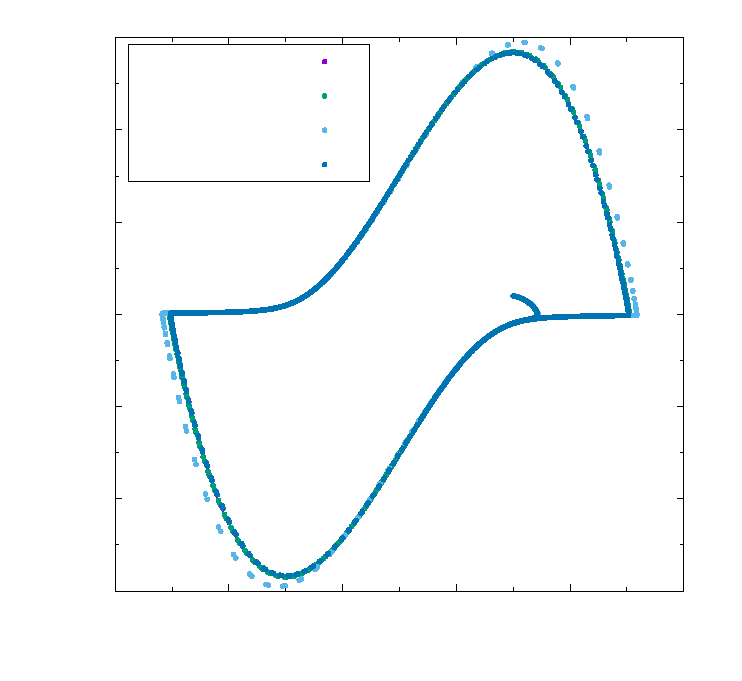
\includegraphics[width={340.10bp},height={311.80bp}]{Comp10}}%
    \gplfronttext
  \end{picture}%
\endgroup

\end{figure}
Alla luce dei confronti che abbiamo appena fatto capiamo che, come atteso, il fatto che la costante di smorzamento, che in questo caso indica anche la rigidità dell'equazione, sia di un'ordine di grandezza più grande richiede anche che i timestep siano un ordine di grandezza più piccoli. Infatti, il timestep "h = 0.1", che con $\mu = 1$ dava risultati approssimativi ma comunque accettabili, con $\mu=10$ è assolutamente insufficiente e presenta lo stesso comportamento che si otteneva usando un timestep $h = 1$ con $\mu = 1$. 
\subsection{Soluzione numerica con il metodo di Runge-Kutta }
Il metodo di Eulero usato preliminarmente è piuttosto impreciso, in particolare vista la rigidità dell'equazione di Van Der Pol, e si vuole quindi trovare una soluzione utilizzando il metodo di Runge-Kutta del secondo ordine, che è molto più preciso. Infatti questo metodo, di solito indicato con $RK2$, ha un ordine di accuratezza 2, a differenza di Eulero che come si è verificato nella sezione precedente ha ordine di accuratezza 1. \\
Il metodo di Runge-Kutta deriva dall'espansione in Taylor dell'equazione differenziale, dove invece che trascurare i termini di ordine superiore a $1$, come si fa nel metodo di Eulero, si considerano anche i termini di ordine $2$. \\ \\
Per l'oscillatore di Van Der Pol si trova il seguente sistema di equazioni:
\begin{equation}
	\begin{cases}
		x_{n+1} = x_n + \frac{1}{2}(k_1 + k_2) \\
		y_{n+1} = y_n + \frac{1}{2}(l_1 + l_2)
	\end{cases}
\end{equation}
dove $k_1$, $k_2$, $l_1$ e $l_2$ sono dei coefficienti definiti da
\begin{equation}
	k_1 = hy_n \ \ \ \ \ \ \ \ \ \ k_2 = h(y_n + l_1) 
\end{equation}
\begin{equation}
	l_1 =  h\left(\mu(1-x_n^2)y _n - x_n\right) \ \ \ \ \  l_2 = h \left[\mu\left(1-(x_n + k_1)^2\right)\left(y_n + l_1\right) - (x_n + k_1)\right]
\end{equation}
dove $h$ è il time-step.
\section{Circuito elettronico}
Per realizzare un circuito che descriva l'equazione di Van Der Pol sono necessari elementi circuitali attivi che appbiano proprietà cubiche non lineare della forma
\begin{equation}
	i = \phi(v) = \gamma V^3 - \alpha V
\end{equation}
dove $i$ è la corrente e $V$ è il voltaggio. \\
In origine Van Der Pol creò il circuito utilizzando una valvola termoionica, o tubo a vuoto, ma dopo l'invenzione del diodo a tunnel è divenuto molto più facile realizzare circuiti di questo tipo. \\
Mediante l'utilizzo di un diodo a tunnel che abbia la caratteristica I-V
\begin{equation}
	i = \phi_t(V) = \phi(V - E_0) + i_0
\end{equation}
l'equazione del circuito prende la forma
\begin{equation}
	\begin{cases}
		\dot{V} = \dfrac{1}{C}\left(-\phi(V) - W\right) \\
		\dot{W} = \dfrac{1}{L}V
	\end{cases} 
\end{equation}
e combinando le due equazioni di questo sistema si ottiene l'equazione differenziale
\begin{equation}
	\ddot{V}-\frac{1}{C}\left( \alpha - 3\gamma  V^2\right)\dot{V} + \frac{1}{LC} = 0
\end{equation}
che è proprio l'equazione di Van Der Pol. Guardando bene l'equazione infatti si vede che l'ultimo termine è proprio il termine oscillativo di un circuito LC, che va a formare un oscillatore armonico elettronico di pulsazione $\omega = 1/\sqrt{LC}$. Il termine di mezzo invece è molto semplicemente riconoscibile come il termine dissipativo non lineare caratteristico dell'oscillatore di Van Der Pol. \\ \\
Quando la costante di smorzamento $\mu$ è grande, il periodo di oscillazione dell'oscillatore è proporzionale a $\mu$, quindi il sistema ha periodo di oscillazione $T \propto \mu\sqrt{LC} = L\alpha$. Dal momento che $\alpha$ equivale all'inverso di una resistenza, si ottiene $T \propto L/r$. Il rapporto $L/R$ è la costante del tempo di rilassamento nei circuiti LR, e questo giustifica il nome "relaxation-oscillation". 
\subsection{Realizzazione di un circuito}
Come detto precedentemente, un possibile circuito elettronico che realizza un oscillatore di Van Der Pol può essere costruito mediante un diodo a tunnel nel modo seguente 
\begin{figure}[H]
	\centering
	\includegraphics[scale=0.4]{NotMycircuit}
	\caption{Circuito con il diodo a tunnel.}
\end{figure}
Non è stato possibile realizzare questo circuito per la mancanza di diodi a tunnel, tuttavia è stato realizzato un circuito alternativo che presenta lo stesso andamento 
\begin{figure}[H]
	\centering
	\includegraphics[scale=0.8]{Mycircuit}
	\caption{Circuito utilizzato nella simulazione su LtSpice.}
\end{figure}
dove si considera una resistenza variabile secondo la formula
\begin{equation}
	R(t) = -\frac{1}{\mu(1 - \frac{V^2(t)}{3})}
\end{equation}
Questo circuito è stato realizzato su LtSpice e mediante la funzione oscilloscopio si è ottenuto il seguente andamento per la tensione:
\begin{figure}[H]
	\centering
	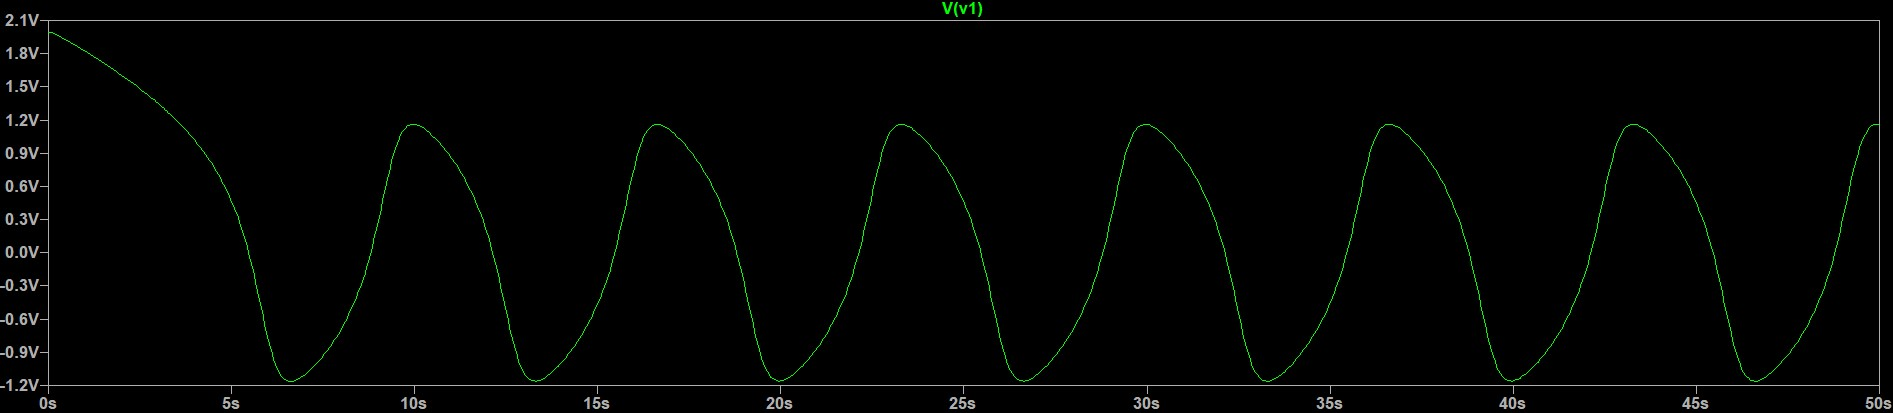
\includegraphics[scale=0.4]{ltspice}
	\caption{Andamento temporale della tensione su LtSpice.}
\end{figure}
che è consistento con l'andamento atteso dal modello di Van Der Pol.
\section{Appendice}
\subsection{Codici per la soluzione dell'equazione Van Der Pol}
\subsubsection{Eulero}
\begin{lstlisting}
	void VDP1(double x0, double y0, double dt, 
	  double mu, double T, std::string s) { 
		double steps = T/dt;
		double x = x0;
		double y = y0;
		double z;
		std::ofstream outfile;
		outfile.open(s);
		
		for(int i = 0; i != steps; ++i) {
			z = x + y*dt;
			y = (mu*(1-pow(x,2))*y - x)*dt + y;
			x = z;
			
			outfile << x << '\t' << y << '\n';
		}
		outfile.close();
	}
	
	void AndTempX(double x0, double y0, double dt, 
	  double mu, double T, std::string s) { 
		double t = 0;
		double steps = T/dt;
		double x = x0;
		double y = y0;
		double z;
		std::ofstream outfile;
		outfile.open(s);
		
		for(int i = 0; i != steps; ++i) {
			z = x + y*dt;
			y = (mu*(1-pow(x,2))*y - x)*dt + y;
			x = z;
			
			outfile << t << '\t' << x << '\n';
			t = t + dt;
		}
		outfile.close();
	}
	
	void AndTempP(double x0, double y0, double dt, 
	  double mu, double T, std::string s) {
		double t = 0;
		double steps = T/dt;
		double x = x0;
		double y = y0;
		double z;
		std::ofstream outfile;
		outfile.open(s);
		
		for(int i = 0; i != steps; ++i) {
			z = x + y*dt;
			y = (mu*(1-pow(x,2))*y - x)*dt + y;
			x = z;
			
			outfile << t << '\t' << y << '\n';
			t = t + dt;
		}
		outfile.close();
	}
\end{lstlisting}
\subsubsection{Runge-Kutta}
\begin{lstlisting}
	void vdpRK(double x0, double y0, double h, 
	  double mu, double T, std::string s) {
		double steps = T/h;
		double x = x0;
		double y = y0;
		double k1,k2,l1,l2;
		double z;
		std::ofstream outfile;
		outfile.open(s);
		
		for(int i = 0; i != steps; ++i) {
			k1 = h*y;
			l1 = h*(mu*(1-pow(x,2))*y - x);
			k2 = h*(y+l1);
			z = x + (k1 + k2)/2;
			l2 = h*(mu*(1-pow(x+k1,2))*(y + l1*h/2) - (x+k1));
			y = y + (l1 + l2)/2;
			x = z;
			
			outfile << x << '\t' << y << '\n';
		}
		outfile.close();
	}
	
	void xRK(double x0, double y0, double h, 
	  double mu, double T, std::string s) {
		double steps = T/h;
		double x = x0;
		double y = y0;
		double k1,k2,l1,l2;
		double z;
		std::ofstream outfile;
		outfile.open(s);
		outfile << 0 << '\t' << x0 << '\n';
		
		for(int i = 0; i != steps; ++i) {
			k1 = h*y;
			l1 = h*(mu*(1-pow(x,2))*y - x);
			k2 = h*(y+l1);
			z = x + (k1 + k2)/2;
			l2 = h*(mu*(1-pow(x+k1,2))*(y + l1*h/2) - (x+k1));
			y = y + (l1 + l2)/2;
			x = z;
			
			outfile << (i+1)*h << '\t' << x << '\n';
		}
		outfile.close();
	}
	
	void pRK(double x0, double y0, double h, 
	  double mu, double T, std::string s) {
		double steps = T/h;
		double x = x0;
		double y = y0;
		double k1,k2,l1,l2;
		double z;
		std::ofstream outfile;
		outfile.open(s);
		outfile << 0 << '\t' << y0 << '\n';
		
		for(int i = 0; i != steps; ++i) {
			k1 = h*y;
			l1 = h*(mu*(1-pow(x,2))*y - x);
			k2 = h*(y+l1);
			z = x + (k1 + k2)/2;
			l2 = h*(mu*(1-pow(x+k1,2))*(y + l1*h/2) - (x+k1));
			y = y + (l1 + l2)/2;
			x = z;
			
			outfile << (i+1)*h << '\t' << y << '\n';
		}
		outfile.close();
	}
\end{lstlisting}
\subsection{Codice per l'accoppiamento dei neuroni}
\begin{lstlisting}
	int main() {    
		double x=0.65,y=-0.65,b=-0.15,d=0.15,z=0.,w=0.;
		float h = 0.01;
		int steps = 10000;
		double T = 4.;
		double e = 0.1;
		
		std::ofstream outfile;
		std::ofstream outfile1;
		outfile.open("Accop.dat");
		outfile1.open("Accop1.dat");
		for(int i = 0; i < steps; ++i) {
			z = -(h/e)*(pow(x,3) - T*x + b) + x;
			b = (x-y)*h + b;
			x = z;
			w = -(h/e)*(pow(y,3) - T*y + d) + y;
			d = (y-x)*h + d;
			y = w;
			
			outfile << x << '\t' << b << '\n';
			outfile1 << y << '\t' << d << '\n';
		}
		outfile.close();
		outfile1.close();
	}
\end{lstlisting}
\subsection{Codice per l'oscillatore forzato}
\begin{lstlisting}
	void Forzato(double x0, double y0, double dt, 
	  double mu, double T, double w,  double A, std::string s) { 
		double steps = T/dt;
		double x = x0;
		double y = y0;
		double z;
		std::ofstream outfile;
		outfile.open(s);
		
		for(int i = 0; i != steps; ++i) {
		  z = x + y*dt;
		  y = y - dt * (x + mu * y * (std::pow(x, 2) - 1) 
		      - A * std::cos(w * t));
		  x = z;
			
		  outfile << x << '\t' << y << '\n';
		}
		outfile.close();
	}
\end{lstlisting}

\section{Bibliografia}
$[1]$ Boccara N. \textit{Modelling complex systems} \\
$[2]$ Rambaldi S. \textit{Dispense sulle equazioni differenziali di primo ordine} \\
$[3]$ Rambaldi S. \textit{Dispense sulle equazioni differenziali del secondo ordine} \\
$[4]$ Wikipedia \textit{Van Der Pol oscillator}\\
$[5]$ Scholarpedia \textit{Van Der Pol oscillator} \\
$[6]$ Wikipedia \textit{FitzHugh-Nagumo model} \\
$[7]$ Scholarpedia \textit{FitzHugh-Nagumo model} 

\end{document}